%!TEX root=./LIVRO.tex

\chapter{Representações numéricas}


\section*{Habilidades do SAEB}

\begin{itemize}
\item
  Escrever números racionais (representação fracionária ou decimal
  finita) em sua representação por algarismos ou em língua materna ou
  associar o registro numérico ao registro em língua materna.
\item
  Compor ou decompor números racionais positivos (representação decimal
  finita) na forma aditiva, ou em suas ordens, ou em adições e
  multiplicações.
\item
  Comparar ou ordenar números reais, com ou sem suporte da reta
  numérica.
\item
  Converter uma representação de um número racional positivo para outra
  representação. 
\item Identificar um número natural como primo, composto,
  ``múltiplo/fator de'' ou ``divisor de'' ou identificar a decomposição
  de um número natural em fatores primos ou relacionar as propriedades
  aritméticas (primo, composto, ``múltiplo/fator de'' ou ``divisor de'')
  de um número natural à sua decomposição em fatores primos.
\end{itemize}



\subsection{Habilidades da BNCC}

\begin{itemize} 
\item EF06MA01, EF06MA05.
\end{itemize}




\conteudo{
\begin{center}
\textbf{Escrever números racionais}
\end{center}

Números racionais incluem frações e números decimais. Frações como 
$\frac{1}{2}$ ou $\frac{3}{4}$ representam partes de um inteiro e podem 
ser escritas usando algarismos ou palavras na língua materna. Além disso, 
essas frações podem ser convertidas em números decimais finitos, 
como $0,5$ ou $0,75$, proporcionando diferentes maneiras de representar a mesma quantidade.

\begin{center}
\textbf{Compor e decompor números racionais}
\end{center}

Ao compor números racionais, podemos somar ou multiplicar partes menores 
para formar números maiores. Por exemplo, $1,25$ é a composição de $1$ e 
$0,25$. A decomposição, por outro lado, envolve dividir um número em partes 
menores. Entender como os números racionais são compostos e decompostos é 
essencial para manipular quantidades de maneira eficaz.

\begin{center}
\textbf{Comparar e ordenar números reais}
\end{center}

A reta numérica é uma ferramenta valiosa que nos ajuda a comparar e ordenar 
números reais. Imagine-a como uma linha infinita em que podemos posicionar 
qualquer número. Comparar números envolve determinar qual número está à esquerda 
ou à direita na reta numérica. Ordenar números significa organizá-los em 
uma sequência, do menor para o maior, permitindo-nos entender relações de magnitude.

\begin{center}
\textbf{Identificar propriedades aritméticas}
\end{center}

Compreender as propriedades dos números naturais, como ser primo, composto, 
múltiplo ou divisor, é fundamental. Identificar a decomposição de números 
naturais em fatores primos ajuda a entender as relações entre diferentes 
números, proporcionando uma visão mais profunda dos conceitos aritméticos.}

\section*{Atividades}

\num{1} Escreva a seguir os números primos entre $2$ e $65$.

\reduline{Os números primos de $2$ a $65$, que devem ser obtidos pela construção
proposta, são: $2$, $3$, $5$, $7$, $11$, $13$, $17$, $19$, $23$, $29$, $31$, $37$, $41$, $43$, $47$, $53$, $59$, $61$.\hfill}\linhas{1}

\num{2} Indique com \textbf{V} as afirmações verdadeiras e com \textbf{F} as afirmações falsas.

\begin{boxlist}
\boxitem{V} O número $2$ é o único número par que é primo.
\boxitem{F} Todos os números ímpares são primos.
\boxitem{F} O número $9$ é primo.
\boxitem{V} O número $121$ possui $3$ divisores.
\boxitem{F} O número $289$ é primo.
\boxitem{V} Um número composto possui mais de $2$ divisores.
\boxitem{V} Um número primo possui $2$ divisores: o $1$ e ele mesmo.
\boxitem{V} Os números $41$, $43$ e $47$ são primos.
\end{boxlist}

\num{3} Decomponha os números em fatores primos.

\begin{escolha}
\item  $100$: \reduline{$2^2 \times 5^2 = 100$\hfill}
\item  $60$: \reduline{$2^2\times 3\times 5 = 60$\hfill}
\item  $225$: \reduline{$3^2\times 5^2 = 225$\hfill}
\item  $1.000$: \reduline{$2^3\times 5^3 = 1.000$\hfill}
\item  $36$: \reduline{$2^2\times 3^2 = 36$\hfill}
\end{escolha}

\num{4} Qual é a decomposição em fatores primos do número $720$?

\reduline{$2^4 \times 3^2 \times 5 = 720$.\hfill}
\linhas{1}

\num{5} Qual é o menor número composto formado pelos fatores primos $2$, $3$, $5$ e $11$?

\reduline{$2 \times 3 \times 5 \times 11 = 330$.\hfill}
\linhas{1}

\num{6}  O número $8$ pode ser fatorado como $8 = 2 \times 2 \times 2 = 2^3$ e, portanto,
possui $3$ fatores primos. O número $30$ também tem $3$ fatores primos, pois
$30 = 2 \times 3 \times 5$. A partir disso, apresente 
números compostos formados por $3$ fatores primos.

\reduline{Possibilidades de resposta: $25$, $49$, $64$, $81$.\hfill}
\linhas{1}

\num{7} Quais números estão representados a seguir?

\begin{escolha}
\item VIII: \reduline{$8$. \hfill}
\item XVII: \reduline{$17$. \hfill}
\item XXIII: \reduline{$23$. \hfill}
\item LIX: \reduline{$59$. \hfill}
\item DXLV: \reduline{$545$. \hfill}
\item MDXCVIII: \reduline{$1.598$. \hfill}
\end{escolha}

\num{8} Explique a diferença entre a representação decimal e
fracionária dos números. Dê exemplos de números e mostre como
eles são representados de forma decimal e fracionária. Explique
também como converter um número decimal em uma fração e vice-versa.

\reduline{A representação dos números pode ocorrer de duas maneiras 
principais: decimal e fracionária. A forma decimal usa a base $10$ 
e separa os números inteiros das partes fracionárias, como em $3,25$,
que representa três inteiros e vinte e cinco centésimos. Por outro
lado, a representação fracionária utiliza frações, como $\frac{13}{4}$,
indicando treze quartos. Para converter um número decimal em fração, 
é preciso identificar as partes inteira e decimal, usando o número 
inteiro como numerador e acrescentando zeros no denominador conforme 
as casas decimais. Para transformar uma fração em número decimal, 
basta dividir o numerador pelo denominador. Por exemplo, o decimal 
$2,75$ corresponde a $\frac{275}{100}$, enquanto a fração $\frac{5}{2}$
é igual a $2,5$ em sua forma decimal. Esses métodos oferecem diferentes
perspectivas sobre a mesma quantidade, permitindo uma compreensão 
flexível e abrangente dos números. \hfill}

\num{9}  Aborde o sistema de numeração romana. Explique como os romanos 
representavam números usando letras e quais são as regras básicas desse 
sistema. Dê exemplos de números e peça aos alunos para escrevê-los em 
algarismos arábicos.

\reduline{O sistema de numeração romana é uma antiga forma de representar 
números utilizada no Império Romano. Nesse sistema, os números são expressos 
por meio de letras do alfabeto latino. As regras básicas incluem a utilização de 
letras como símbolos numéricos, como $I$ para $1$, $V$ para $5$, $X$ para $10$,
$L$ para $50$, $C$ para $100$, $D$ para $500$ e $M$ para $1.000$. A representação 
romana segue princípios específicos, como a adição e a subtração para formar 
números. Quando uma letra de menor valor está à esquerda de uma letra de maior 
valor, subtrai-se o valor menor do maior; quando está à direita, adiciona-se. 
Por exemplo, $IV$ representa $4$ ($1$ subtraído de $5$) e $XC$ representa $90$
($10$ subtraído de $100$). Essa representação pode parecer complexa, mas é uma
parte essencial da história matemática e cultural. \hfill}

\num{10}  O número $35.482$ pode ser decomposto nas parcelas $30.000 + 5.000 +
400 + 80 + 2$. Seguindo esse mesmo raciocínio, decomponha os números a seguir.

\begin{escolha}
\item $9.876$.

\reduline{$9.000 + 800 + 70 + 6$.\hfill}
\item $12.345$.

\reduline{$10.000 + 2.000 + 300 + 40 + 5$.\hfill}
\item $678.912$.

\reduline{$600.000 + 70.000 + 8.000 + 900 + 10 + 2$.\hfill}
\item $60.504$.

\reduline{$60.000 + 500 + 4$.\hfill}
\end{escolha}

\section*{Treino}

\num{1} O maior cometa já descoberto é o Holmes, que possui $2.251$ km de
diâmetro. Quantas ordens possui o número que representa o diâmetro do cometa?

\begin{escolha}
\item Duas ordens.
\item Três ordens.
\item Quatro ordens.
\item Dez ordens.
\end{escolha}


% Comparar, ordenar, ler e escrever números naturais e
% números racionais cuja representação decimal é finita, fazendo uso da
% reta numérica.

% SAEB: Compor ou decompor números racionais positivos (representação
% decimal finita) na forma aditiva, ou em suas ordens, ou em adições e
% multiplicações.

% Gabarito
% Alternativa A: incorreta, pois o aluno pode ter uma mal interpretação e
% contar as classes ao invés das ordens.
% Alternativa B: incorreta, pois o aluno pode ter uma mal interpretação e
% considerar que as ordens são um conjunto de $3$ números após o ponto.
% Alternativa C: correta, pois são $4$ ordens ao total.
% Alternativa D: incorreta, pois o aluno pode compreender que ordens são a
% soma de todos os números descritos.

\num{2} José tem $IX$ anos de idade; seu irmão mais velho, $XXI$ anos; 
o mais novo, $V$. Somando a idade dos três, encontramos a idade do pai.
Quantos anos tem o pai dos garotos?

\begin{escolha}
\item $XXV$.
\item $XXXV$.
\item $XXXVII$.
\item $XXX$.
\end{escolha}

\begin{figure}[H]
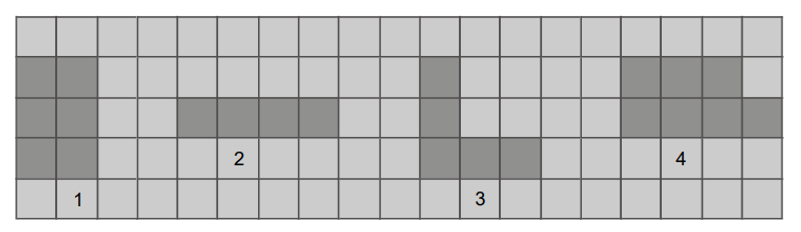
\includegraphics[width=\textwidth]{imgSAEB_6_MAT/media/image133.png}
\end{figure}

%\subsection{BNCC: EF06MA05}

% SAEB: Converter uma representação de um número racional positivo para
% outra representação.
% -- Classificar números naturais em primos e compostos,
% estabelecer relações entre números, expressas pelos termos ``é múltiplo
% de'', ``é divisor de'', ``é fator de'', e estabelecer, por meio de
% investigações, critérios de divisibilidade por $2$, $3$, $4$, $5$, $6$, $8$, $9$, $10$,
% 100 e $1000$.

% Gabarito
% Alternativa A: incorreta, o aluno pode esquecer de somar um ``X''.
% Alternativa B: correta, pois essa é a representação em numerais romanos.
% Alternativa C: incorreta, o aluno pode compreender que IX é $11$ ao invés
% de $9$.
% Alternativa D: incorreta, o aluno pode esquecer de somar a idade do
% irmão mais novo.

\num{3}  O algarismo romano $MMMDCCXVII$ representa o número decimal

\begin{escolha}
\item $3.225$.
\item $3.717$.
\item $3.718$.
\item $3.417$.
\end{escolha}

%\subsection{BNCC: EF06MA01 }

% -- Comparar, ordenar, ler e escrever números naturais e
% números racionais cuja representação decimal é finita, fazendo uso da
% reta numérica.
% SAEB: Converter uma representação de um número racional positivo para
% outra representação.

% Gabarito
% Alternativa A: incorreta, pois o aluno pode considerar que a letra ``D''
% representa ``Dezena'', logo o valor seria esse.
% Alternativa B: correta, pois essa é a representação dos números.
% Alternativa C: incorreta, pois o aluno pode confundir e contar um ``I''
% a mais e considerar que o valor correto é esse.
% Alternativa D: incorreta, pois o aluno pode considerar que a letra D
% signifique Duzentos, logo o resultado seria esse.

\chapter{Operações aritméticas}

\section*{Habilidades do SAEB}

\begin{itemize}
\item Calcular o resultado de adições, subtrações,
multiplicações ou divisões envolvendo número reais. 
\item Calcular o
resultado de potenciação ou radiciação envolvendo números reais.
\item Resolver problemas de adição, subtração, multiplicação, divisão,
  potenciação ou radiciação envolvendo número reais, inclusive notação
  científica.
\item Resolver problemas de contagem cuja resolução envolva a aplicação do
  princípio multiplicativo. - Resolver problemas que envolvam as ideias
  de múltiplo, divisor, máximo divisor comum ou mínimo múltiplo comum.
\end{itemize}

\subsection{Habilidades da BNCC}
\begin{itemize} 
\item  EF06MA06, EF06MA07, EF06MA10, EF06MA11.
\end{itemize}



\conteudo{Cada termo entre o sinal de $+$ é denominado \textbf{parcela}. O valor representado
após o sinal de $=$ é denominado \textbf{soma} ou \tetxbf{total}. Veja:

$$100 + 500 = 600$$

Trata-se da adição.

Já na subtração, o primeiro termo da operação deverá, necessariamente, ser o de maior
valor. Ele é chamado de \textbf{minuendo}. Já o \textbf{subtraendo}, isto é, o número
menor, deverá aparecer na segunda posição. O número encontrado após o
sinal de igual é denominado \textbf{resto} ou \textbf{diferença}. Veja:

$$300 - 100 = 200$$

Na multiplicação, cada um do dois números sendo multiplicados é denominado de \textbf{fator}. 
O resultado da operação se chama \textbf{produto}. Veja:

$$4 \times 10 = 40$$

Quanto à divisão, o primeiro número da operação é chamado de \textbf{dividendo}. O número é
seguinte é o \textbf{divisor}. O resultado é denominado \textbf{quociente}. Veja:

$$81 \div 9 = 9$$}

\section*{Atividades}

\num{1} Um agricultor colheu $358$ kg de maçãs e $247$ kg de peras de sua fazenda. 
Ele vendeu $112$ kg de maçãs para o mercado local e $75$ kg de peras para um supermercado.

\begin{escolha}
\item Quanta fruta o agricultor colheu no total?

\rosa{A quantidade total de frutas}

\rosa{colhidas pelo agricultor é a}

\rosa{soma de maçãs e peras colhidas:}

\rosa{$358 + 247 = 605$ kg de frutas.}

\item Quantos quilogramas de maçãs e peras ele ainda tem depois de vender parte da colheita?

\rosa{Maçãs restantes:}

\rosa{$358 - 112 = 246$ kg de maçãs.}

\rosa{Peras restantes:}

\rosa{$247 - 75 = 172$ kg de peras.}

\item Se o agricultor planeja fazer cestas de frutas com $5$ kg de maçãs e $4$ kg de peras cada,
quantas cestas ele poderá fazer com a quantidade restante de frutas?

\rosa{Para fazer cestas de frutas,}

\rosa{o agricultor poderá fazer:}

\rosa{Número de cestas de maçãs:}

\rosa{$246 \div 5 = 49$ cestas de maçãs.}

\rosa{Número de cestas de peras:}

\rosa{$172 \div 4 = 43$ cestas de peras.}
\end{escolha}

\num{2}  Enzo tinha $R\$284,00$ e ganhou de seu pai uma nota de $R\$50,00$. Qual é
o valor total que ele tem agora?

\reduline{$334$ reais.\hfill}

\num{3}  Em um supermercado, há uma balança informando o peso dos alimentos
ali colocados. Aurora pesou suas compras e observou o seguinte resultado
no visor da balança:

\begin{figure}
\centering
\includegraphics[width=2.33333in,height=1.53125in]{./imgSAEB_6_MAT/media/image23.png}
\end{figure}

Após observar o resultado, decidiu pegar mais um item com o peso de
$225$ g. Após colocar o item na balança, qual é o novo valor observado?

\reduline{$875 + 225 = 1.090$ kg. \hfill}

\num{4}  A coleção de Celso tem $91$ bolas de gude, e a de Marcelo, $112$. Quantas
bolas de gude os dois possuem juntos?

\reduline{$91 + 112 = 203$ bolinhas de gude.\hfill}

\num{5}  Uma biblioteca municipal contém $3.697$ livros. Considerando que $391$
livros estão emprestados, quantos livros restam nas estantes dessa
biblioteca?

\reduline{$3.697 - 391 = 3.306$ livros.\hfill}

\num{6}  No início da semana, uma lanchonete tinha $530$ latas de refrigerante.
Ao longo da semana, foram vendidas $371$ latas. Quantas latas restaram na
lanchonete?

\reduline{$530 - 371 = 159$ latinhas.\hfill}

\num{7}  Utilizando o método de decomposição em fatores primos, calcule o M.M.C. entre os números a seguir.

\begin{escolha}
\item $52$ e $78$.

\reduline{$156$.\hfill}
\item $8$, $10$ e $14$.

\reduline{$280$.\hfill}
\item $18$ e $42$.

\reduline{$126$.\hfill}
\item $12$ e $48$.

\reduline{$48$.\hfill}
\item $90$ e $180$.

\reduline{$180$.\hfill}
\end{escolha}

\num{8}  Utilizando o método de decomposição em fatores primos, calcule o MDC entre os números a seguir.

\begin{escolha}
\item $52$ e $78$.

\reduline{$78$.\hfill}
\item $8$, $10$ e $14$.

\reduline{$2$.\hfill}
\item $32$ e $48$.

\reduline{$16$.\hfill}
\item $60$ e $72$.

\reduline{$12$.\hfill}
\end{escolha}

\num{9} Joana comprou $3$ rolos de tecido:

\begin{itemize}
\item O primeiro mede $100$ cm;
\item O segundo mede $80$ cm;
\item O terceiro mede $120$ cm.
\end{itemize}

Ela pretende dividir os rolos em
pedaços iguais e do maior tamanho possível. Sendo assim, quantos pedaços
terá cada pedaço de tecido?

\rosa{Para determinar quantos pedaços iguais de tecido Joana pode obter de cada rolo, é necessário encontrar o maior divisor comum (MDC) dos comprimentos dos rolos. Calculamos o MDC dos comprimentos dos três rolos:

1. Primeiro, vamos fatorar os números em seus fatores primos:

\(100 = 2^2 \times 5^2\)

\(80 = 2^4 \times 5^1\)

\(120 = 2^3 \times 3^1 \times 5^1\)

O MDC é obtido pegando os menores expoentes de cada fator primo presente em todos os números:

Para \(2\), o menor expoente é \(2^2 = 4\).

Para \(3\), não há \(3\) em todos os números.

Para \(5\), o menor expoente é \(5^1 = 5\).

Agora, multiplicamos esses fatores primos juntos para encontrar o MDC: \(MDC = 2^2 \times 5^1 = 20\).

Portanto, Joana pode cortar cada rolo em pedaços de \(20 \, \text{cm}\) de comprimento.}

\num{10} Laura, Pablo e Josiane trabalham em uma empresa de turismo e viajam
constantemente para o Nordeste. Laura viaja de $10$ em $10$ dias, Pablo de
$15$ em $15$ dias e Josiane, de $20$ em $20$ dias. Se todos forem hoje para o
Nordeste, daqui a quanto tempo eles viajarão no mesmo dia novamente?

\rosa{Para descobrir quando Laura, Pablo e Josiane viajarão no mesmo dia novamente, precisamos encontrar o menor múltiplo comum (MMC) dos intervalos em que cada um viaja.

Primeiro, vamos decompor os números em seus fatores primos:

\(10 = 2^1 \times 5^1\)

\(15 = 3^1 \times 5^1\)

\(20 = 2^2 \times 5^1\)

O MMC é obtido pegando os maiores expoentes de cada fator primo presente em todos os números:

Para \(2\), o maior expoente é \(2^2 = 4\).

Para \(3\), o maior expoente é \(3^1 = 3\).

Para \(5\), o maior expoente é \(5^1 = 5\).

Agora, multiplicamos esses fatores primos juntos para encontrar o MMC:

\[ MMC = 2^2 \times 3^1 \times 5^1 = 60 \]

Portanto, Laura, Pablo e Josiane viajarão no mesmo dia novamente daqui a $60$ dias.}

\num{11} Um tabuleiro de xadrez é todo quadriculado e composto de $8$ linhas e
$8$ colunas. Cada quadradinho é chamado de casa. Quantas casas tem esse
tabuleiro?

% Tabela
% https://pixabay.com/pt/vectors/tabuleiro-de-xadrez-xadrez-conselho-29630/.

\reduline{$8 \cdot 8 = 64$ casas.\hfill}

\num{12} Calcule as potências a seguir.

\begin{escolha}
\item $5^2$: \reduline{$25$.\hfill}
\item $3^2$: \reduline{$9$.\hfill}
\item $4^3$: \reduline{$64$.\hfill}
\item $7^2$: \reduline{$49$.\hfill}
\item $2^3$: \reduline{$8$.\hfill}
\item $10^3$: \reduline{$1000$.\hfill}
\item $3^3$: \reduline{$27$.\hfill}
\item $8^2$: \reduline{$64$.\hfill}
\end{escolha}

% \noindent É interessante explorar a operação potenciação por meio de
% situações-problema. Exemplo:

% \begin{itemize}
% \item Em um estacionamento há $4$ automóveis, em cada automóvel há $4$ rodas e
% em cada roda há $4$ parafusos. Qual é o total de parafusos desses $4$
% automóveis?

% \item Um fazendeiro armazena as laranjas de sua fazenda para vender em
% caixas que lembram um cubo. Cada caixa contém $5$ laranjas no comprimento,
% 5 laranjas na largura e $5$ laranjas na altura. Quantas laranjas podem ser
% armazenadas em $5$ caixas?
% \end{itemize}

% Professor
% Observar as estratégias dos alunos para resolver as situações propostas.
% É possível que alguns optem em fazer desenhos, esquemas ou optem pelo
% material concreto para auxiliá-los no cálculo.

% Associe essas atividades com a representação de uma
% potenciação. Inicialmente, a linguagem utilizada para definir a
% potenciação e seus elementos pode ser confusa para os alunos. Sempre que
% possível, fazer a identificação desses elementos utilizando exemplos ou
% atividades para que eles possam compreender a nomenclatura correta e as
% ideias ligadas a essa simbologia.

\section*{Treino}

\num{1}  Três asteroides se aproximam do sol a cada $20$, $24$, e $28$ anos,
respectivamente. Se o último ano em que todos estiveram próximos do sol
foi $1984$, o próximo ano em que isso deverá ocorrer será

\begin{escolha}
\item
  $1992$
\item
  $2840$
\item
  $2988$
\item
  $3664$
\end{escolha}

%\subsection{BNCC: EF06MA06 }
% -- Resolver e elaborar problemas que envolvam as ideias
% de múltiplo e de divisor.
% SAEB: Resolver problemas que envolvam as ideias de múltiplo, divisor,
% máximo divisor comum ou mínimo múltiplo comum.

% Gabarito
% Alternativa A: incorreta, pois o aluno pode realizar a somar a soma ao
% invés de calcular o M.\,M.\,C.
% Alternativa B: incorreta, pois o aluno pode considerar que o valor do
% M.\,M.\,C. em si já é a resposta.
% Alternativa C: incorreta, pois o aluno pode confundir M.\,M.\,C. com M.\,D.\,C.
% nos cálculos e chegar a esse resultado.
% Alternativa D: correta, pois somando o resultado do M.\,M.\,C. com o ano de
% 1984 obtemos este valor.

\num{2}  Entre algumas famílias foram distribuídos $240$ cadernos, $576$ lápis e
$1.080$ borrachas. A distribuição foi feita de tal modo que o maior número
de famílias fosse contemplado e que cada família recebesse o mesmo
número de lápis, o mesmo número de cadernos e o mesmo número de
borrachas. Nessas condições o número de borrachas que cada família
recebeu foi

\begin{escolha}
\item $24$.
\item $8$.
\item $12$. 
\item $45$.
\end{escolha}

%\subsection{BNCC: EF06MA07 }
% -- Compreender, comparar e ordenar frações associadas às
% ideias de partes de inteiros e resultado de divisão, identificando
% frações equivalentes.
% SAEB: Resolver problemas que envolvam as ideias de múltiplo, divisor,
% máximo divisor comum ou mínimo múltiplo comum.

% Gabarito
% Alternativa A: incorreta, pois O aluno pode confundir o resultado do
% M.\,D.\,C. dos valores como resposta.
% Alternativa B: incorreta, pois o aluno pode calcular incorretamente o
% M.\,D.\,C. esquecendo do valor $5$ no final, onde o resultado seria esse.
% Alternativa C: incorreta, pois o aluno pode esquecer de contar um número
% ``2'' no cálculo do M.\,D.\,C.
% Alternativa D: correta, pois, calculando o M.\,D.\,C., obtemos $24$,
% realizando a operação $1080$: $24$ obtemos $45$.

\num{3}  Jonas abastece seu veículo a cada $3$ dias e Moisés a cada $6$. Paulo vai
abastecer seu veículo sempre aos sábados e em nenhum outro dia. Se, no
dia $20$ de setembro, os dois abasteceram seus veículos, a próxima data em
que os três abastecerão juntos será

\begin{escolha}
\item $20$ de outubro.
\item $2$ de novembro.
\item $1$ de novembro.
\item $31$ de Outubro.
\end{escolha}

%\subsection{BNCC: EF06MA06 }
% -- Resolver e elaborar problemas que envolvam as ideias
% de múltiplo e de divisor.
% SAEB: Resolver problemas que envolvam as ideias de múltiplo, divisor,
% máximo divisor comum ou mínimo múltiplo comum.

% Gabarito
% Alternativa A: incorreta, pois o aluno pode considerar correta essa
% alternativa caso ele considere que se encontram no mesmo dia de todo
% mês.
% Alternativa B: incorreta, pois o aluno pode chegar a esse resultado se
% considerar que outubro tenha $30$ dias.
% Alternativa C: correta, pois realizando o M.\,M.\,C., temos $42$ dias. $20$ dias
% depois de $20$ de setembro cairá no dia $1$ de novembro, lembrando que
% outubro tem $31$ dias.
% Alternativa D: incorreta, pois o aluno pode considerar que setembro
% tenha $31$ dias.

\chapter{Frações}
\markboth{Módulo 3}{}

\section*{Habilidades do SAEB}
\begin{itemize}
\item Representar frações menores ou maiores que a
unidade por meio de representações pictóricas ou associar frações a
representações pictóricas.
\item
  Identificar frações equivalentes.
\item
  Determinar uma fração geratriz para uma dízima periódica.
\end{itemize}

\subsection{Habilidade da BNCC} 
\begin{itemize}
\item EF06MA09.
\end{itemize}

\conteudo{
Uma fração é uma forma de representar uma quantidade ou uma proporção de
um todo que é dividido em partes iguais. Ela é composta de duas partes:
o \textbf{numerador} e o \textbf{denominador}. O numerador representa a quantidade ou a
parte que está sendo considerada, e o denominador representa o total de
partes em que o todo foi dividido.

Por exemplo, a fração $\frac{3}{4}$ representa a parte de um todo que é igual a
três partes em um total de quatro partes iguais. Isso pode ser
visualizado como uma pizza dividida em quatro partes iguais, em que três
dessas partes são consideradas.

As frações podem ser usadas em diversas situações, como na representação
de números decimais em forma de fração, na resolução de problemas que
envolvem proporções ou na medição de quantidades em que um todo é
dividido em partes iguais, como no caso de receitas culinárias.

As frações também podem ser comparadas e operadas matematicamente
por meio de adição, subtração, multiplicação e divisão, o que permite
realizar cálculos e resolver problemas que envolvem frações.

% Tabela
% https://br.freepik.com/fotos-gratis/graficos-estatisticos-coloridos-para-fracoes-cientificas\_6626366.htm\#query=fractions\&from\_query=fra\%C3\%A7\%C3\%B5es\&position=6\&from\_view=search\&track=sph.
% Acesso em: $5$ maio $2023$.

A comparação entre frações significa olhar para duas frações e descobrir
qual é a maior ou qual é a menor. Para comparar frações, é necessário
deixá-las com o mesmo denominador e ver qual tem o maior numerador.

Por exemplo, a fração $\frac{2}{3}$ é maior que a fração $\frac{1}{3}$, pois o numerador
(isto é, o número de cima) é maior. Perceba como o número da parte
inferior da fração, o denominador, é o mesmo.

As frações equivalentes são aquelas que, embora aparentemente pareçam
diferentes, possuem o mesmo resultado. Sendo assim, elas representam a
mesma parte de um todo, indicando a mesma quantidade.

Por exemplo, a fração $\frac{1}{2}$ é equivalente à fração $\frac{2}{4}$. Para nos
certificarmos desse fato, basta dividirmos o numerador e denominador da
segunda fração por $2$, chegando à fração $\frac{1}{2}$ novamente.}

% Resgatar com os alunos os conhecimentos que possuem acerca das frações,
% para assim aproximar ou relembrar conceitos estudados anteriormente. Se
% possível, levar figuras de círculos de cartolina para que os alunos
% possam vivenciar as questões propostas nesta seção. Eles podem dividir
% as representações dos círculos em pedaços e recortá-los como se fossem
% pizzas e realizar diferentes explorações. Vale destacar que é
% interessante refletir com os alunos sobre o uso de alimentos para
% representar frações, pois muitas vezes uma fatia pode possuir o mesmo
% tamanho que outras, mas as massas podem ser diferentes.}

\section*{Atividades}

\num{1}  Dois irmãos, Pedro e Joel, resolveram comprar uma pizza juntos. Ao
chegar em casa, Pedro comeu $\frac{3}{8}$ da pizza, enquanto Joel comeu $\frac{7}{16}$.
Qual dos irmãos comeu a maior parte da pizza?

\reduline{Joel comeu a maior quantidade de pizza, pois $\frac{3}{8} < \frac{7}{16}$.\hfill}
\linhas{1}

\num{2}  João tem um bolo de chocolate que ele quer dividir igualmente entre seus 4 amigos. 
Se o bolo inteiro representa $\frac{3}{4}$ de um quilograma, quanto de bolo cada amigo 
receberá? Explique como você chegou à resposta e simplifique a fração, se necessário.

\rosa{Para resolver esse problema, primeiro, precisamos encontrar a quantidade de bolo}

\rosa{que cada amigo receberá. Sabemos que o bolo inteiro representa $\frac{3}{4}$ de um quilograma.}

\rosa{Para dividir igualmente entre 4 amigos, precisamos dividir $\frac{3}{4}$ por $4$:}

\rosa{$\frac{3}{4} \div 4 = \frac{3}{4} \times \frac{1}{4} = \frac{3 \times 1}{4 \times 4} = \frac{3}{16}$}

\rosa{Portanto, cada amigo receberá $\frac{3}{16}$ de um quilograma de bolo de chocolate.}

\num{3} Maria gastou $\frac{3}{8}$ de seu salário em um novo computador 
e $\frac{1}{6}$ do restante em livros. Se ela ainda tem R\$ 500,00 sobrando,
qual é o valor do salário total de Maria? Explique os passos para encontrar a resposta.

\rosa{Para resolver esse problema, precisamos primeiro calcular}

\rosa{a fração do salário que Maria gastou no computador e nos livros.}

\rosa{Maria gastou $\frac{3}{8}$ de seu salário no computador;}

\rosa{então o restante do salário é $1 - \frac{3}{8} = \frac{5}{8}$ do total do salário.}

\rosa{Em seguida, Maria gastou $\frac{1}{6}$ do restante em livros.}

\rosa{Então, a parte do salário que sobrou após comprar o computador}

\rosa{foi $\frac{5}{8} \times \frac{1}{6} = \frac{5}{48}$ do total do salário.}

\rosa{Sabemos que essa quantia é igual a R\$ 500,00. Portanto podemos configurar a equação:}

\rosa{$\frac{5}{48} \times \text{salário total} = 500$}

\rosa{Para encontrar o valor do salário total, multiplicamos ambos os lados da equação por}

\rosa{$\frac{48}{5}$ para isolar o salário total: $\text{salário total} = 500 \times \frac{48}{5} = 4.800$}

\rosa{Assim, o salário total de Maria é R\$ 4.800,00.}

\num{4} Para ser aprovado em uma prova, Lucas precisava acertar no mínimo $\frac{3}{5}$
das questões. Ao final do teste, Lucas descobriu que acertou $\frac{2}{3}$ das questões.
Sendo assim, ele foi aprovado ou reprovado? Explique.

\reduline{Lucas foi aprovado, pois $\frac{2}{3} > \frac{3}{5}$.\hfill}
\linhas{1}

% \num{5} Sabendo que as figuras foram divididas em partes iguais, em cada
% item, escreva a fração correspondente à parte colorida de amarelo.

% \begin{figure}
% 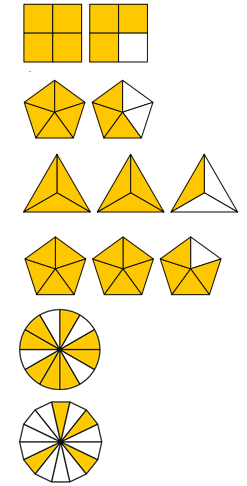
\includegraphics[width=0.7\textwidth]{./imgSAEB_6_MAT/media/image32.png}
% \end{figure}

% \begin{escolha}
% \item \reduline{$7/4$.\hfill}
% \item \reduline{$8/5$.\hfill}
% \item \reduline{$7/3$.\hfill}
% \item \reduline{$14/5$.\hfill}
% \item \reduline{$8/12$.\hfill}
% \item \reduline{$4/14$.\hfill}
% \end{escolha}

% \noindent Nestas atividades, reforçar a ideia de fração como parte de um todo.
% Quando se trabalha com sua representação geométrica, há necessidade de
% fazer a divisão do todo em partes iguais. Quais elementos podem ser representados por meio de uma fração?

\num{5}  Simplifique as frações, tornando-as irredutíveis.

\begin{escolha}
\item $\frac{24}{60}$ 

\reduline{$\frac{2}{5}$.\hfill}
\item $\frac{18}{90}$ 

\reduline{$\frac{1}{5}$.\hfill}
\item $\frac{27}{36}$ 

\reduline{$\frac{3}{4}$.\hfill}
\item $\frac{63}{81}$ 

\reduline{$\frac{7}{9}$.\hfill}
\item $\frac{9}{81}$ 

\reduline{$\frac{1}{9}$.\hfill}
\item $\frac{7}{21}$ 

\reduline{$\frac{1}{3}$.\hfill}
\item $\frac{60}{80}$ 

\reduline{$\frac{3}{4}$.\hfill}
\end{escolha}

\num{6}  Maria resolveu fazer bolos para vender em sua padaria. Em cada
receita, são utilizados $\frac{3}{4}$ de xícara de farinha de trigo. Em um final
de semana, Maria faz $8$ bolos. Quantas xícaras foram necessárias?

\rosa{Cada receita usa $\frac{3}{4}$ de xícara de farinha de trigo.}

\rosa{Para 8 bolos, a quantidade necessária é:}

\rosa{$\text{Quantidade de farinha de trigo} = \left( \frac{3}{4} \text{ xícaras de farinha} \right) \times 8 \text{ bolos}$}

\rosa{$\text{Quantidade de farinha de trigo} = \frac{3}{4} \times 8 \text{ xícaras de farinha}$}

\rosa{$\text{Quantidade de farinha de trigo} = 6 \text{ xícaras de farinha}$}

\rosa{Portanto, Maria precisou de $6$ xícaras de farinha de trigo para fazer os $8$ bolos.}

\num{7}  Leonardo resolveu pintar um quadro simples para colocar na parede de
seu quarto. Para pintar o quadro, Leonardo utilizou as cores azul e laranja.
Observer a imagem.

\begin{figure}[H]
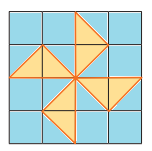
\includegraphics[width=1.58333in,height=1.57292in]{./imgSAEB_6_MAT/media/image33.png}
\end{figure}

Qual das duas Leonardo usou mais?

\reduline{Leonardo usou no seu quadro $\frac{12}{16}$ de tinta azul e $\frac{4}{16}$ de
tinta laranja. Como $\frac{12}{16} > \frac{4}{16}$, ele usou mais a tinta
azul.\hfill}

\num{8}  Represente por meio de frações.

\begin{figure}
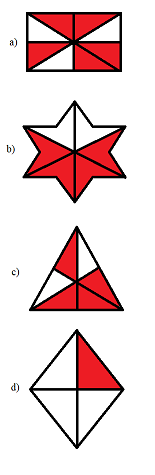
\includegraphics[width=1.61458in,height=4.94792in]{./imgSAEB_6_MAT/media/image34.png}
\end{figure}

\begin{escolha}
\item \reduline{$\frac{5}{8}$.\hfill}
\item \reduline{$\frac{6}{8}$.\hfill}
\item \reduline{$\frac{4}{6}$.\hfill}
\item \reduline{$\frac{1}{4}$.\hfill}
\end{escolha}

% Professor
% Deixar o espaço de $1$ linhas abaixo de cada item para resolução e inserir
% a figura descrita acima, podendo ser uma figura semelhante a essa, porém
% contendo o mesmo conteúdo fracionário.

\num{9} Um prêmio em dinheiro foi dividido entre $4$ amigos em partes
fracionárias. Pedro recebeu $\frac{1}{6}$ do valor, Henrique recebeu $\frac{1}{2}$, Josias
recebeu $\frac{1}{4}$ e Adriano, $\frac{1}{12}$ . Qual dos quatro amigos recebeu a maior
parte do prêmio?

\rosa{Para comparar as frações, precisamos encontrar um denominador comum.}

\rosa{O menor múltiplo comum de $6$, $2$, $4$ e $12$ é $12$.}

\rosa{\textbf{Pedro}: $\frac{1}{6} \times \frac{2}{2} = \frac{2}{12}$}

\rosa{\textbf{Henrique}: $\frac{1}{2} \times \frac{6}{6} = \frac{6}{12}$}

\rosa{\textbf{Josias}: $\frac{1}{4} \times \frac{3}{3} = \frac{3}{12}$}

\rosa{\textbf{Adriano}: $\frac{1}{12} \times \frac{1}{1} = \frac{1}{12}$}

\rosa{Comparando as frações, podemos ver que Henrique recebeu a maior parte do prêmio,}

\rosa{já que $\frac{6}{12} > \frac{3}{12} > \frac{2}{12} > \frac{1}{12}$}

\section*{Treino}

\num{1}  Em uma padaria, há uma torta que pode ser dividida em $8$ pedaços
iguais. João comeu $3$ desses pedaços, e Maria comeu $\frac{2}{4}$ da torta.
O que se pode afirmar corretamente sobre essa situação?

\begin{escolha}
\item João comeu mais torta.
\item Maria comeu mais torta.
\item João e Maria comeram a mesma quantidade de torta.
\item Não é possível determinar a resposta, pois as frações são diferentes.
\end{escolha}


%\subsection{BNCC: EF06MA09 }
% -- Resolver e elaborar problemas que envolvam o cálculo
% da fração de uma quantidade e cujo resultado seja um número natural, com
% e sem uso de calculadora.
% SAEB: Representar frações menores ou maiores que a unidade por meio de
% representações pictóricas ou associar frações a representações
% pictóricas.

% Gabarito
% Alternativa A: incorreta, pois o aluno provavelmente efetuou a operação
% de maneira incorreta.
% Alternativa B: correta, pois $2/4 = (2 x 2) / (4 x 2) = 4/8$
% $3/8$; logo, Maria comeu mais torta.
% Alternativa C: incorreta, pois a operação demonstra que Maria e João
% comeram porções diferentes.
% Alternativa D: incorreta, pois o aluno deve saber comparar frações
% diferentes.

\num{2}  Um jogo matemático é formado por cartas com frações impressas em uma
de suas faces. Cada jogador recebe quatro cartas e vence aquele que
primeiro conseguir ordená-las crescentemente pelas respectivas frações
impressas. O vencedor foi o aluno que recebeu as cartas com as seguintes frações:

$$\frac{3}{5}, \frac{1}{4}, \frac{2}{3} e \frac{5}{9}$$

A ordem que esse aluno apresentou foi:

\begin{escolha}
\item $\frac{1}{4}$, $\frac{5}{9}$, $\frac{3}{5}$, $\frac{2}{3}$.
\item $\frac{1}{4}$, $\frac{2}{3}$, $\frac{3}{5}$, $\frac{5}{9}$.
\item $\frac{5}{9}$, $\frac{1}{4}$, $\frac{3}{5}$, $\frac{2}{3}$.
\item $\frac{5}{9}$, $\frac{1}{4}$, $\frac{3}{5}$, $\frac{2}{3}$.
\end{escolha}

%\subsection{BNCC: EF06MA09 }
% -- Resolver e elaborar problemas que envolvam o cálculo
% da fração de uma quantidade e cujo resultado seja um número natural, com
% e sem uso de calculadora.
% SAEB: Identificar frações equivalentes.

% Gabarito
% \begin{figure}
% 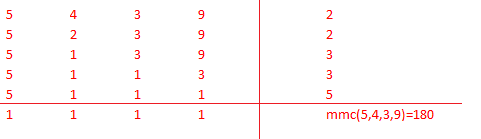
\includegraphics[width=5.01042in,height=1.44792in]{./imgSAEB_6_MAT/media/image36.png}
% \end{figure}

% \noindent Para encontrar as frações equivalentes, dividimos $180$ pelos
% denominadores das frações sorteadas e, multiplicamos o resultado pelos
% numeradores.

% Para $3/5$
% \begin{itemize}
% $180 / 5 = 36$, como $36 x 3 = 108$, a fração equivalente será $108 / 180$.
% \end{itemize}
% Para $1/4$
% \begin{itemize}
% $180/4 = 45$, como $45 x 1 = 45$, a fração equivalente será $45/180$
% \end{itemize}
% Para $2/3$
% \begin{itemize}
% $180/3 = 60$, como $60 x 2 = 120$, a fração equivalente será $120/180$
% \end{itemize}
% Para $5/9$
% \begin{itemize}
% $180/9 = 20$, como $20 x 5 = 100$. A fração equivalente será $100/180$
% \end{itemize}

% Com as frações equivalentes, basta ordenar pelos numeradores em ordem
% crescente e associar com as frações sorteadas. Logo $1/4$, $5$/9, $3/5$, $2/3$.

% Alternativa A: correta, pois: Para comparar frações elas devem possuir os denominadores iguais. Para isso, calculamos o MMC entre $5$, $4$, $3$ e $9$, que são os denominadores das frações sorteadas.
% Alternativa B: incorreta, O aluno pode considerar que quanto maior o
% denominador, maior o valor fracionário, assim $1/4$ seria uma fração maior
% que $2/3$.
% Alternativa C: incorreta, o aluno pode se confundir na forma de calcular
% o M.\,M.\,C. e colocar erroneamente as frações de forma incorreta.
% Alternativa D: incorreta, o aluno pode se confundir e colocar as frações
% em forma decrescente ao invés de crescente.

\num{3}  Elias comprou dois potes de sorvete, ambos com a mesma quantidade do
produto. Um dos potes continha quantidades iguais dos sabores chocolate,
creme e morango; o outro, quantidades iguais dos sabores chocolate e
baunilha. Então, nessa compra, a fração total
correspondente à quantidade de sorvete do sabor chocolate foi

\begin{escolha}
\item $\frac{2}{6}$. 
\item $\frac{3}{5}$. 
\item $\frac{5}{12}$. 
\item $\frac{5}{6}$.
\end{escolha}

%\subsection{BNCC: EF06MA09 }
% -- Resolver e elaborar problemas que envolvam o cálculo
% da fração de uma quantidade e cujo resultado seja um número natural, com
% e sem uso de calculadora.
% SAEB: Representar frações menores ou maiores que a unidade por meio de
% representações pictóricas ou associar frações a representações
% pictóricas

% Gabarito
% Alternativa A: incorreta, pois o aluno pode erroneamente considerar que
% ambos os potes de sorvete foram divididos em $3$ partes.
% Alternativa B: incorreta, pois o aluno erroneamente pode considerar que
% somando as partes de chocolates de ambos os potes sem calcular o M.\,M.\,C.
% pode se tornar uma resposta correta.
% Alternativa C: correta, pois: o primeiro pote continha $3$ sabores em
% iguais quantidades: $1/3$ de chocolate, $1/3$ de baunilha e $1/3$ de morango.
% No segundo pote, havia $1/2$ de chocolate e $1/2$ de baunilha. Considerando
% os dois potes de sorvete, dividimos os dois potes em partes iguais.
% Fazendo então o M.\,M.\,C. de (2,3), obtemos que cada pote foi dividido em $6$
% partes iguais. Portanto nos dois potes temos $12$ partes iguais. Sendo que
% destas, $5$ partes correspondem ao sabor chocolate.
% Alternativa D: incorreta, o aluno pode considerar dividir os potes em $3$
% partes iguais e somar sem calcular o M.\,M.\,C., que chegará a esse
% resultado erroneamente.

\chapter{Porcentagem}
\markboth{Módulo 4}{}

\section*{Habilidade do SAEB} 
\begin{itemize}
\item Resolver problemas que envolvam porcentagens,
incluindo os que lidam com acréscimos e decréscimos simples, aplicação
de percentuais sucessivos e determinação de taxas percentuais.
\end{itemize}

\subsection{Habilidade da BNCC} 
\begin{itemize}
\item EF06MA13.
\end{itemize}

\conteudo{Porcentagem é uma forma de expressar uma proporção ou uma parte de um
todo em termos de uma base de $100$ unidades. O símbolo ``\%'' é usado
para indicar porcentagem. Por exemplo, se uma empresa tem $100$
funcionários e $50$ deles são mulheres, podemos dizer que $50\%$ dos
funcionários são mulheres. A porcentagem é amplamente utilizada em
finanças, negócios, estatísticas, ciência, entre outras áreas, para
expressar a parte de um todo ou uma taxa de crescimento ou decréscimo em
relação a uma base de $100$.

Acréscimo é o aumento em um valor, que pode ser
expresso em valores absolutos ou em porcentagem.
Por exemplo, se o preço de um produto é R\$ 100,00, e houve um acréscimo
de $10\%$, o novo preço será R\$ 110,00. O cálculo do preço com acréscimo é
feito multiplicando o preço original pela porcentagem de acréscimo (em
forma decimal), e adicionando o resultado ao preço original, Veja:

$$\text{Preço com acréscimo} = \text{Preço original} + (\text{Preço original} \times \text{Porcentagem de acréscimo})$$

Desconto é uma redução no preço de um produto ou serviço, geralmente
oferecida como uma forma de incentivar as vendas ou recompensar os
clientes. O desconto é expresso em porcentagem e é aplicado ao preço
original do produto ou serviço.

Por exemplo, se um produto tem um preço original de R\$ 100,00, e há um
desconto de $20\%$, o preço com desconto será R\$ 80,00. O cálculo do preço
com desconto é feito multiplicando o preço original pela porcentagem de
desconto (em forma decimal), e subtraindo o resultado do preço original.}

\section*{Atividades}

\num{1} Calcule as porcentagens a seguir.

\begin{escolha}
\item $1\%$ de $120$.

\reduline{$1,2$.\hfill}

\item $50\%$ de $260$.

\reduline{$130$.\hfill}

\item $10\%$ de $1300$.

\reduline{$130$.\hfill}

\item $25\%$ de $9$.

\reduline{$2,25$.\hfill}

\item $30\%$ de $120$.

\reduline{$36$.\hfill}

\item $5\%$ de $90$.

\reduline{$4,5$.\hfill}

\item $2\%$ de $310$.

\reduline{$6,2$.\hfill}

\item $45\%$ de $195$.

\reduline{$87,75$.\hfill}

\item $33\%$ de $125$.

\reduline{$41,25$.\hfill}

\item $90\%$ de $1700$.

\reduline{$1530$.\hfill}

\item $70\%$ de $1745$.

\reduline{$1221,5$.\hfill}

\item $0,5\%$ de $205$.

\reduline{$1,025$.\hfill}

\item $2,5\%$ de $25$.

\reduline{$0,625$.\hfill}

\end{escolha}

\num{2} Marly tem um salário atual de $R\$ 1.250,00$. Seu novo patrão irá
aumentar seu salário em $15\%$. Qual será o valor do novo salário dela?

\reduline{$R\$ 1.437,50$.\hfill}
\linhas{2}

\num{3} Uma televisão em uma loja de departamentos custa $R\$ 3.800,00$.
Como José adquiriu uma TV e efetuou pagamento à vista, recebeu um
desconto no valor de $15\%$ no produto. Nessas condições, qual foi a
quantia paga por José?

\reduline{$R\$ 3.230,00$.\hfill}
\linhas{2}

\num{4} Uma universidade resolveu iniciar uma pesquisa para saber o perfil
dos alunos. Foi descoberto que $46\%$ dos alunos são homens. Sabendo
que a faculdade possui $1.250$ alunos, quantas mulheres estudam nessa
universidade?

\rosa{Se $46\%$ dos alunos são homens,}

\rosa{$54\%$ dos alunos são mulheres. Logo:}

\rosa{$\text{Número de mulheres} = \frac{54}{100} \times \text{Número de alunos}$}

\rosa{$\text{Número de mulheres} = \frac{54}{100} \times 1.250$}

\rosa{$\text{Número de mulheres} = \frac{54 \times 1.250}{100}$}

\rosa{$\text{Número de mulheres} = \frac{67.500}{100}$}

\rosa{São, portanto, $675$ alunas na universidade.}

\num{5} O campeonato brasileiro de futebol possui $38$ rodadas. Para cada
vitória, a equipe ganha $3$ pontos. Sendo assim, a pontuação máxima a ser
alcançada é de $114$ pontos. Sabendo que a equipe vencedora do ano de 2022
obteve $81$ pontos, qual é a porcentagem de pontos alcançada?

\rosa{Para encontrar a porcentagem de pontos alcançada pela equipe vencedora}

\rosa{do Campeonato Brasileiro de Futebol em 2022, podemos usar a fórmula:}

\rosa{$\text{Porcentagem de pontos} = \left( \frac{\text{Pontuação obtida}}{\text{Pontuação máxima possível}} \right) \times 100\%$}

\rosa{A pontuação obtida pela equipe vencedora foi de $81$ pontos,}

\rosa{e a pontuação máxima possível é de $114$ pontos. Logo:}

\rosa{$\text{Porcentagem de pontos} = \left( \frac{81}{114} \right) \times 100\%$}

\rosa{De $\frac{81}{114}$, obtemos $\frac{9}{12}$, que pode ser simplificada para $\frac{3}{4}$.}

\rosa{Então, a porcentagem de pontos alcançada pela equipe vencedora foi:}

\rosa{$\left( \frac{3}{4} \right) \times 100\% = 75\%$}

\rosa{A equipe vencedora do Campeonato Brasileiro de Futebol em 2022 alcançou $75\%$ da pontuação máxima possível.}

\num{6} Em janeiro, um brinquedo custava $R\$ 90,00$. Devido à queda nas
vendas, seu preço sofreu uma redução de $20\%$, mantendo-se esse valor até
novembro. Com o aquecimento das vendas de Natal, houve um aumento de
$10\%$. O brinquedo passou a ser vendido por quanto?

\reduline{O brinquedo passou a ser vendido por $R\$ 79,20$.\hfill}
\linhas{2}

\num{7}  Uma pesquisa constatou que, no ano de 2021, uma cidade do interior de
São Paulo possuía $25.000$ habitantes. Considerando que, no ano de 2022,
houve um aumento de $6\%$ na população, quantos habitantes havia nessa
cidade no ano de 2022?

\reduline{Em 2022, a população dessa cidade era de $26.500$ habitantes.\hfill}
\linhas{2}

\num{8}  Elias foi ao supermercado e constatou que o pacote de arroz de $5$ kg
custava $R\$ 21,50$. No mês seguinte, o mesmo produto custava $R\$ 23,10$.
Qual foi o acréscimo, em porcentagem?

\rosa{$\text{Acréscimo percentual} = \left( \frac{\text{Preço final} - \text{Preço inicial}}{\text{Preço inicial}} \right) \times 100\%$}

\rosa{$\text{Acréscimo percentual} = \left( \frac{23,10 - 21,50}{21,50} \right) \times 100\%$}

\rosa{Calculando o numerador $(23,10 - 21,50)$, obtemos $1,60$. Substituindo esse valor na fórmula:}

\rosa{$\text{Acréscimo percentual} = \left( \frac{1,60}{21,50} \right) \times 100\%$}

\rosa{Calculando o denominador $(1,60 / 21,50)$, obtemos, aproximadamente, $0,0744$.}

\rosa{Multiplicando por $100$ para obter a porcentagem:}

\rosa{$\text{Acréscimo Percentual} \approx 0,0744 \times 100\% \approx 7,44\%$}

\rosa{Portanto, o acréscimo no preço do pacote de arroz foi de aproximadamente $7,44\%$.}

\num{9} Em uma loja, o preço de determinado par de calçados era
$R\$ 120,00$. Durante uma liquidação, ele era vendido por $R\$ 81,00$. Em
relação ao preço original, o desconto dado corresponde a uma taxa de quanto?

\rosa{Para encontrar a taxa de desconto em relação ao preço original, podemos usar a fórmula:}

\rosa{$\text{Taxa de desconto} = \left( \frac{\text{Desconto}}{\text{Preço original}} \right) \times 100\%$}

\rosa{O desconto dado é a diferença entre o preço original e o preço de liquidação:}

\rosa{$\text{Desconto} = 120,00 - 81,00 = 39,00$}

\rosa{$\text{Taxa de desconto} = \left( \frac{39,00}{120,00} \right) \times 100\%$}

\rosa{Calculando o numerador $(39,00 / 120,00)$, obtemos, aproximadamente, $0,325$.}

\rosa{Multiplicando por 100 para obter a porcentagem:}

\rosa{$\text{Taxa de Desconto} \approx 0,325 \times 100\% \approx 32,5\%$}

\rosa{O desconto dado durante a liquidação corresponde a uma taxa de $32,5\%$ em relação ao preço original do par de calçados.}

\num{10}  Uma loja oferece $10\%$ de desconto na compra de $1$ produto, $20\%$ na
compra de $2$ produtos e $30\%$ na compra de $3$ produtos. Adriano quer
comprar camisas com o preço unitário de $R\$80,00$. Quanto Adriano
pagaria

\begin{escolha}
\item na compra de apenas $1$ camisa?

\reduline{Adriano pagaria $90\%$ do preço original de uma camisa, já que há um desconto de $10\%$. O preço original de uma 
camisa é R\$80,00.
Para calcular o preço com desconto, multiplicamos o preço original pela porcentagem após o desconto:
$\text{Preço com desconto} = 80,00 \times 0,90 = 72,00 \, \text{R\$}$
Portanto, Adriano pagaria R\$ 72,00 na compra de apenas 1 camisa.\hfill}

\item na compra de $2$ camisas?

\reduline{Para calcular o preço que Adriano pagaria na compra de apenas 2 camisas, precisamos levar em consideração o desconto 
de 20\% oferecido na compra de 2 produtos.
O preço original de uma camisa é R\$ 80,00. Com um desconto de 20\% na compra de 2 camisas, o preço com desconto para cada camisa será:
$\text{Preço com desconto} = 80,00 \times 0,80 = 64,00 \, \text{R\$}$
Então, Adriano pagaria R\$ 64,00 por cada uma das 2 camisas.\hfill}

\item na compra de $3$ camisas?

\reduline{Para calcular o preço que Adriano pagaria na compra de três camisas, precisamos levar em consideração o desconto de 
30\% oferecido na compra de três produtos.
O preço original de uma camisa é R\$80,00. Com um desconto de 30\% 
na compra de 3 camisas, o preço com desconto para cada camisa será:
$\text{Preço com desconto} = 80,00 \times 0,70 = 56,00 \, \text{R\$}$
Então, Adriano pagaria R\$56,00 por cada uma das 3 camisas.\hfill}
\end{escolha}

\num{11}  Uma pessoa comprou um terreno por R\$ 20.000,00 e o vendeu com o
lucro de R\$ 4.000,00. Qual foi a porcentagem de lucro?

\rosa{Para calcular a porcentagem de lucro, podemos usar a seguinte fórmula:}

\rosa{$\text{Porcentagem de Lucro} = \left( \frac{\text{Lucro}}{\text{Custo}} \right) \times 100\%$}

\rosa{No caso, o lucro é R\$4.000,00 e o custo (ou preço de compra) é R\$20.000,00. Substituindo esses valores na fórmula, temos:}

\rosa{$\text{Porcentagem de Lucro} = \left( \frac{4000}{20000} \right) \times 100\%$}

\rosa{Calculando o numerador \(4000 / 20000\), obtemos \(0,2\). Multiplicando por 100 para obter a porcentagem:}

\rosa{$\text{Porcentagem de Lucro} = 0,2 \times 100\% = 20\%$}

\rosa{Portanto, a pessoa obteve um lucro de \(20\%\) ao vender o terreno.}

\section*{Treino}

\num{1}  Em determinada cidade, as passagens de ônibus custavam $R\$ 1,20$. O
novo prefeito reajustou esse valor em $25\%$. Qual será o novo valor das
passagens?

\begin{escolha}
\item $R\$ 1,45$.
\item $R\$ 1,23$.
\item $R\$ 1,25$.
\item $R\$ 1,50$.
\end{escolha}

%\subsection{BNCC: EF06MA13 }
% -- Resolver e elaborar problemas que envolvam
% porcentagens, com base na ideia de proporcionalidade, sem fazer uso da
% ``regra de três'', utilizando estratégias pessoais, cálculo mental e
% calculadora, em contextos de educação financeira, entre outros.
% SAEB: Resolver problemas que envolvam porcentagens, incluindo os que
% lidam com acréscimos e decréscimos simples, aplicação de percentuais
% sucessivos e determinação de taxas percentuais.

% Gabarito
% Alternativa A: incorreta, pois o aluno pode considerar que aumentar $25\%$
% signifique aumentar $25$ centavos.
% Alternativa B: incorreta, pois o aluno pode calcular erroneamente $1,20$ x
% 0,025, chegando a esse resultado equivocado.
% Alternativa C: incorreta, poiso aluno pode considerar que $25\%$ tenha
% relação com o valor $R\$1,25$, pela semelhança.
% Alternativa D: correta, pois $R\$1,20 x 0,25 = 0,3$, logo somando $R\$1,20$
% + $R\$0,30$ temos $1,50$

\num{2}  Uma livraria realizará uma liquidação e, para isso, o gerente pediu
para Ariane multiplicar todos os preços dos livros por $0,68$. Nessa
liquidação, a loja está oferecendo um desconto de:

\begin{escolha}
\item $68\%$.
\item $6,8\%$.
\item $3,2\%$.
\item $32\%$.
\end{escolha}

%\subsection{BNCC: EF06MA13 }
% -- Resolver e elaborar problemas que envolvam
% porcentagens, com base na ideia de proporcionalidade, sem fazer uso da
% ``regra de três'', utilizando estratégias pessoais, cálculo mental e
% calculadora, em contextos de educação financeira, entre outros.
% SAEB: Resolver problemas que envolvam porcentagens, incluindo os que
% lidam com acréscimos e decréscimos simples, aplicação de percentuais
% sucessivos e determinação de taxas percentuais.

% Alternativa A: incorreta, pois aluno pode deduzir que ao multiplicar o
% valor por $0,68$ que o valor logo terá $68\,\%$ de desconto.
% Alternativa B: incorreta, pois o aluno pode deduzir que, ao multiplicar
% o valor por $0,68$, os livros terão $6,8\,\%$ devido à semelhança dos termos.
% Alternativa C: incorreta, pois o cálculo pode ser feito corretamente mas
% a semelhança de $3,2\%$ para $32\%$ pode confundir o aluno na hora de
% decisão de assinalar a resposta correta.
% Alternativa D: correta, pois, ao multiplicar qualquer valor de livro por
% 68\%, obtém-se um desconto de $32\%$.

\num{3}  Em uma loja, uma máquina de lavar roupas custava $R\$ 1.500,00$, e seu
preço sofreu um aumento de $3\%$. Logo após o aumento, a loja resolveu
fazer uma promoção oferecendo um desconto de $3\%$ no mesmo produto. Qual
era o valor do produto após o aumento? E, após o desconto, ou seja, após as
duas operações?

\begin{escolha}
\item $R\$ 1.555,00$ com aumento e $R\$ 1.498,65$ com desconto.
\item $R\$ 1.545,00$ com aumento e $R\$ 1.500,00$ com desconto.
\item $R\$ 1.545,00$ com aumento e $R\$ 1.498,65$ com desconto.
\item $R\$ 1.555,00$ com aumento e $R\$ 1.500,00$ com desconto.
\end{escolha}

%\subsection{BNCC: EF06MA13 }
% -- Resolver e elaborar problemas que envolvam
% porcentagens, com base na ideia de proporcionalidade, sem fazer uso da
% ``regra de três'', utilizando estratégias pessoais, cálculo mental e
% calculadora, em contextos de educação financeira, entre outros.
% SAEB: Resolver problemas que envolvam porcentagens, incluindo os que
% lidam com acréscimos e decréscimos simples, aplicação de percentuais
% sucessivos e determinação de taxas percentuais.

% Gabarito:
% Alternativa A: incorreta, pois o aluno pode realizar o cálculo
% corretamente, mas confundir os valores próximos de R\$1.555, $00$ com
% R\$1.545, $00$ devido à semelhança.
% Alternativa B: incorreta, pois o aluno, por meio de dedução, pode
% considerar que, somando $3\%$ ao valor inicial e subtraindo $3\%$, o valor
% inicial fique inerte.
% Alternativa C: Correta. Cálculo do acréscimo: $1500\times 0,03 = 45$; $1.550 + 45 = 1.545$. Cálculo do desconto: $1.545\times 0,03 = 46,35$; $1.545 - 46,35 = 1.498,65$.
% Alternativa D: incorreta, pois o aluno, por meio de dedução, pode
% considerar que, somando $3\%$ ao valor inicial e subtraindo $3\%$, o valor
% inicial fique inerte.

\chapter{Equações polinomiais}
\markboth{Módulo 5}{}

\section*{Habilidades do SAEB} 
\begin{itemize}
\item Resolver uma equação polinomial de 1º grau.
\item
 Resolver uma equação polinomial de 1º grau.
\item
  Inferir uma equação, inequação polinomial de 1º grau ou um sistema de
  equações de 1º grau com duas incógnitas que modela um problema.
\item
  Associar uma equação polinomial de 1º grau com duas variáveis a uma
  reta no plano cartesiano.
\item
  Resolver problemas que possam ser representados por sistema de
  equações de 1º grau com duas incógnitas.
\end{itemize}

\subsection{Habilidades da BNCC}
\begin{itemize} 
\item  EF06MA14.
\end{itemize}

\vspace{A equação do 1º grau é uma equação que possui uma incógnita com grau 1,
ou seja, a incógnita está elevada a potência 1. Veja:

$$a \cdot x + b = 0$$

Sendo $a$ e $b$ números reais, e $a$ diferente de $0$.

É dado o sistema:

$$x + y = 40$$
$$3x + 4y = 144$$

Enumeramos as equações:

$$I x + y = 40$$
$$II 3x + 4y = 144$$

Escolhemos a primeira equação e isolamos o $x$:

$$x + y = 40 x = 40 - y$$

Agora, na equação II, substituímos o valor de $x = 40 - y$.

$$3x + 4y = 144$$ 
$$3 (40 - y) + 4y = 144 120 - 3y + 4y = 144 y = 24$$

Descobrimos o valor de $y$. Para descobrir o valor de $x$, basta substituir
o $y$ na equação:

$$x = 40 - y x = 40 - 24 x = 16$$

Portanto, a solução do sistema é $S = (16, 24)$.
}

\section*{Atividades}

\num{1}  Resolva as equações polinomiais a seguir e descubra o valor de x em
cada uma delas.

\begin{escolha}
\item $x + 5 = 8$ \rosa{$3$}
\item $x − 4 = 3$ \rosa{$7$}
\item $x + 9 = −1$ \rosa{$-10$}
\item $4x − 9 = 23$ \rosa{$8$}
\item $7x − 33 = −12$ \rosa{$3$}
\item $33+ x = 5 -- 3x$ \rosa{$-7$}
\item $3(x + 2) = 2 (x - 7)$ \rosa{$-20$}
\item $2x - 10 + 7x + 10 = 180$ \rosa{$20$}
\end{escolha}

\begin{mdframed}[linewidth=2pt,linecolor=white,roundcorner=10pt]
\vspace{6cm}
\end{mdframed}

\num{2}  Responda às sentenças a seguir.

\begin{escolha}
\item O dobro de um número somado com $5$ é igual a $91$. Qual é esse número? \rosa{$x = 43$.}
\item O triplo de um número diminuído de $4$ é igual a $23$. Qual é esse número? \rosa{$x = 9$.}
\item O número somado com o seu dobro é igual a $150$. Qual é esse número? \rosa{$x = 50$.}
\item Qual é o número que, adicionado a $28$, é igual a $3$ vezes esse número? \rosa{$x = 14$.}
\item O triplo de um número menos $10$ é igual ao próprio número mais $70$. Qual é esse número? \rosa{$x = 40$.}
\item Noêmia é $5$ anos mais velha que Ágata. A soma das idades dá $43$ anos. Qual a idade de Ágata? \rosa{Ágata tem $19$ anos.}
\item Quando Manoel nasceu, Carlos tinha $3$ anos. Atualmente, a soma das idades é $23$ anos. Qual é a idade de Carlos? \rosa{Carlos tem $13$ anos.}
\end{escolha}

\begin{mdframed}[linewidth=2pt,linecolor=white,roundcorner=10pt]
\vspace{6cm}
\end{mdframed}

\num{3}  Os $1.200$ alunos matriculados numa escola estão assim distribuídos: no
período da manhã, há $320$ alunos a mais do que no período da tarde e, à
noite, há $190$ alunos a menos do que no período da manhã. Qual é o número de
alunos do período da manhã dessa escola?

\rosa{Vamos usar variáveis para representar o número de alunos em cada período:

\rosa{Seja $x$ o número de alunos no período da tarde.

\rosa{No período da manhã, há $x + 320$ alunos.

\rosa{À noite, há $x - 190$ alunos.

\rosa{Sabemos que o número total de alunos na escola é 1.200.}

\rosa{Portanto, podemos escrever a equação: $x + (x + 320) + (x - 190) = 1.200$}

\rosa{Agora, podemos resolver para $x$:}

\rosa{$3x + 130 = 1.200$}

\rosa{$3x = 1.070$}

\rosa{$x = 356$}

\rosa{Assim, o número de alunos no período da tarde é $356$.}

\rosa{Portanto, o número de alunos no período da manhã é $356 + 320 = 676$.}

\num{4}  Resolva os sistemas formados pelas equações a seguir.

\begin{escolha}
\item $x + y = 1$; $4x + 7y = 10$ \rosa{$x = -1, y = 2$.}
\item $3x + y = 13$; $x - 2y = 2$ \rosa{$x = 4, y = 2$.}
\item $2x + y = 5$; $x - y = 1$ \rosa{$x = 1, y = 2$.}
\item $x + y = 4$; $3x + 2y = 9$ \rosa{$x = 2, y = 1$.}
\item $x + y = 10$; $2x - y = 8$ \rosa{$x = 1, y = 3$.}
\end{escolha}

\begin{mdframed}[linewidth=2pt,linecolor=white,roundcorner=10pt]
\vspace{6cm}
\end{mdframed}

\num{5} Em determinado mês, duas montadoras produziram, juntas, $77.500$
veículos, sendo que a produção de x foi igual a $\frac{2}{3}$ da produção de y.
Nesse mês, qual foi a quantidade de veículos produzidos pela montadora x?

\rosa{Vamos usar variáveis para representar a produção de cada montadora:}

\rosa{$x$ representará a produção da montadora x.}

\rosa{$y$ representará a produção da montadora y.}

\rosa{Sabemos que a produção total foi de $77.500$ veículos. Logo: $x + y = 77.500$}

\rosa{Além disso, a produção de $x$ foi igual a $\frac{2}{3}$ da produção de $y$:}

\rosa{$x = \frac{2}{3}y}

\rosa{Substituindo a segunda equação na primeira, obtemos:}

\rosa{$\frac{2}{3}y + y = 77.500$}

\rosa{Multiplicando todos os termos por $3$ para eliminar o denominador:}

\rosa{$2y + 3y = 232.500$}

\rosa{$5y = 232.500$}

\rosa{$y = 46.500$}

\rosa{$x = \frac{2}{3} \times 46.500$}

\rosa{$x = 31.000$}

\num{6} Numa cantina, $2$ copos de suco e $3$ pastéis custam R\$ 5,70. O preço de
$3$ copos de suco e $5$ pastéis é R\$ 9,30. Quanto custa cada pastel e cada
copo de suco?

\rosa{Vamos usar variáveis para representar o preço de cada pastel e de cada copo de suco.}

\rosa{Seja $x$ o preço de cada pastel em reais.}

\rosa{Seja $y$ o preço de cada copo de suco em reais.}

\rosa{1. $2x + 3y = 5,70$}

\rosa{2. $3x + 5y = 9,30$}

\rosa{A partir da primeira equação, podemos isolar $x$:}

\rosa{$x = \frac{5,70 - 3y}{2}$}

\rosa{$3\left(\frac{5,70 - 3y}{2}\right) + 5y = 9,30$}

\rosa{$3(5,70 - 3y) + 10y = 18,60$}

\rosa{$17,10 - 9y + 10y = 18,60$}

\rosa{$y = 1,50$}

\rosa{$2x + 3 \times 1,50 = 5,70$}

\rosa{$2x + 4,50 = 5,70$}

\rosa{$2x = 1,20$}

\rosa{$x = 0,60$}

\rosa{Portanto, cada pastel custa R\$ 0,60 e cada copo de suco custa R\$ 1,50.}

\num{7}  Considerando a equação $5(3x - 8) = -45$, o que
é correto afirmar sobre uma equação equivalente a ela?

\reduline{É equivalente a equeção $15x + 5 = 0$.\hfill}
\linhas{2}

\num{8}  Uma região retangular foi totalmente cercada por uma tela. Os lados
da região medem $x$ m e $x + 4$ m.
Se para cercar totalmente essa região foram utilizados $24$ m de tela, a
medida do lado menor é igual a:

% \begin{figure}
% \centering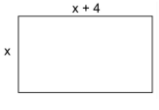
\includegraphics[width=1.65625in,height=1.14583in]{./imgSAEB_6_MAT/media/image38.png}
% \end{figure}

\begin{mdframed}[linewidth=2pt,linecolor=white,roundcorner=10pt]
\rosa{$4$.}
\vspace{6cm}
\end{mdframed}

\num{9} Numa loja, algumas camisetas e calças estão em oferta. $3$ calças e $2$
camisetas são vendidas por $R\$ 56,00$. Por sua vez, $2$ calças e $1$ camiseta
saem por $R\$ 34,00$. O preço unitário da calça e da camiseta pode ser
determinado a partir da solução de qual sistema?

\begin{mdframed}[linewidth=2pt,linecolor=white,roundcorner=10pt]
\rosa{$3x + 2y = 56$}

\rosa{$2x + y = 34$}
\vspace{6cm}
\end{mdframed}

\section*{Treino}

\num{1}  Numa caixa, há bolas vermelhas e bolas amarelas num total de $360$
esferas. Se o número de bolas vermelhas é o quádruplo do de amarelas, o
número de bolas vermelhas é

\begin{escolha}
\item $18$.
\item $72$.
\item $90$.
\item $288$.
\end{escolha}

%\subsection{BNCC: EF06MA14 }
% -- Reconhecer que a relação de igualdade matemática não
% se altera ao adicionar, subtrair, multiplicar ou dividir os seus dois
% membros por um mesmo número e utilizar essa noção para determinar
% valores desconhecidos na resolução de problemas.
% SAEB: Resolver problemas que possam ser representados por sistema de
% equações de 1º grau com duas incógnitas.

% Gabarito
% Alternativa A: incorreta, pois o aluno pode chegar à conclusão de que o
% número de bolas vermelhas é $72$, dividindo por $4$ ao tentar encontrar o
% número de bolas amarelas.
% Alternativa B: incorreta, pois o aluno pode considerar que o enunciado
% pede o número de bolas amarelas.
% Alternativa C: incorreta, pois o aluno pode realizar a operação $360$:4,
% obtendo um resultado incorreto.
% Alternativa D: correta, pois, realizando o sistema, temos que: $X + Y = 360$; $X = 4y$. Inserindo o valor de X na primeira equação, temos que: $4y + y = 360$; $5y = 360$; $y = 72$. Realizando $360 - 72 = 288$, temos o valor correto de bolas vermelhas.

\num{2}  O tempo $t$, em segundos, que uma pedra leva para cair de uma altura $x$,
em metros, é dado aproximadamente pela fórmula $t = 0,05$x. Se o tempo $t$
da queda é de $8$ segundos, a altura $x$ é de

\begin{escolha}
\item $0,4$ m.
\item $0,00625$ m.
\item $160$ m.
\item $4$ m.
\end{escolha}

%\subsection{BNCC: EF06MA14 }
% -- Reconhecer que a relação de igualdade matemática não
% se altera ao adicionar, subtrair, multiplicar ou dividir os seus dois
% membros por um mesmo número e utilizar essa noção para determinar
% valores desconhecidos na resolução de problemas.
% SAEB: Resolver problemas que possam ser representados por sistema de
% equações de 1º grau com duas incógnitas.

% Gabarito
% Alternativa A: incorreta, pois o aluno durante a resolução pode
% confundir e ao invés de dividir $8$ por $0,05$, realizar a multiplicação.
% Alternativa B: incorreta, pois o aluno pode resolver a equação
% erroneamente, calculando $0,05$ : $8$.
% Alternativa C: correta, pois, ao substituir t por $8$, temos: $$8 = 0,05 . x$$; $$8/0,05 = x$$; $$x = 160$$.
% Alternativa D: incorreta, pois o aluno pode erroneamente colocar o valor
% 8 na incógnita x.

\num{3}  Dois produtos químicos A e B são usados em um laboratório. Cada $1$ grama
do produto A custa $R\$ 0,03$, e cada $1$ grama do produto B custa R\$ 0,05.
Se $100$ gramas de uma mistura dos dois produtos custam $R\$ 3,60$, a
quantidade do produto A contida nessa mistura é

\begin{escolha}
\item $70$ gramas.
\item $100$ gramas.
\item $360$ gramas.
\item $140$ gramas.
\end{escolha}

%\subsection{BNCC: EF06MA14 }
% -- Reconhecer que a relação de igualdade matemática não
% se altera ao adicionar, subtrair, multiplicar ou dividir os seus dois
% membros por um mesmo número e utilizar essa noção para determinar
% valores desconhecidos na resolução de problemas.
% SAEB: Resolver problemas que possam ser representados por sistema de
% equações de 1º grau com duas incógnitas.

% Gabarito
% Alternativa A: Correta. Considerando que x = quantidade do produto A em gramas; y = quantidade do produto B em gramas. $x + y = 100$ (I); $x·A + y·B = 3,60$ (II). De (I), deduzimos: $y = 100 - x$. Que aplicamos em (II): $x·A + (100-x)·B = 3,60$. Substituindo A e B pelos seus custos em reais: $x·0,03 + (100-x)y·0,05 = 3,60$. Multiplicando toda a equação acima por $100$, a fim de tornar inteiros
% seus coeficientes: $x·3 + (100-x)·5 = 360$; $3x + 500 - 5x = 360$; $-2x = 360 - 500$; $-2x = -140$; $x = -140/-2$; $x = 70$ gramas. 
% Alternativa B: incorreta, pois o aluno pode simplesmente retirar a
% quantidade de gramas do enunciado e considerar como resposta correta.
% Alternativa C: incorreta, pois o aluno pode considerar o preço final do
% produto como resposta correta.
% Alternativa D: incorreta, pois o aluno pode esquecer de dividir a
% equação final por $2$, chegando a esse resultado.

\chapter{Proporções}
\markboth{Módulo 6}{}

\section*{Habilidade do SAEB} 
\begin{itemize}
\item Resolver problemas que envolvam variação de
proporcionalidade direta ou inversa entre duas ou mais grandezas,
inclusive escalas, divisões proporcionais e taxa de variação.
\end{itemize}

\conteudo{Veja alguns tipos de razão:

\noindent\textbf{Escala}\quad
\noindent A razão de escala é uma relação matemática que indica a proporção
entre as dimensões de duas figuras semelhantes. Ela é dada pela razão
entre as medidas de um mesmo lado (ou altura ou diagonal etc.) das
duas figuras.

Por exemplo, se duas figuras são semelhantes e o lado da primeira figura
mede $5$ cm e o lado correspondente da segunda figura mede $10$ cm, a razão
de escala entre as duas figuras é $\frac{10}{5}$ ou $\frac{2}{1}$.

\noindent\textbf{Velocidade média}\quad
Velocidade média é uma grandeza física que representa a
variação de espaço (distância percorrida) em relação ao tempo gasto para
percorrê-lo. Ela é dada pela razão entre a distância percorrida e o
tempo gasto: $\text{Velocidade média} = \frac{\text{Distância percorrida}}{\text{Tempo gasto}}$.

\noindent\textbf{Densidade}\quad
Densidade é uma grandeza física que representa a quantidade de
massa presente em determinado volume. Ela é calculada pela razão
entre a massa de um objeto e o volume ocupado por ele. A fórmula da densidade é:
$\text{Densidade} = \frac{\text{Massa}}{\text{Volume}}$

\noindent\textbf{Densidade demográfica}\quad
\noindent A densidade demográfica é uma medida que indica a
relação entre a população de uma área e a sua superfície.
Ela é obtida dividindo-se o número de habitantes pela área total da
região.
Por exemplo, se uma cidade tem uma população de $100.000$ habitantes e sua
área total é de $50$ km², sua densidade demográfica é de $2.000$ habitantes
por quilômetro quadrado.

Todos esses tipos de razão podem seguir uma lógica direta ou
inversamente proporcional.}

\section*{Atividades}

\num{1}  Para se construir uma calçada, é comum, na constituição do concreto,
utilizar cimento, areia e brita na seguinte proporção: $1$ parte de
cimento, $4$ partes de areia e $2$ partes de brita. Para construir a
calçada, uma construtora encomendou um caminhão betoneira com $14$ m³ de
concreto. Qual é o volume de cimento, em metro cúbicos, na carga de concreto
trazida pela betoneira?

\begin{mdframed}[linewidth=2pt,linecolor=white,roundcorner=10pt]
\rosa{$2$ m³.}
\vspace{6cm}
\end{mdframed}

\num{2}  Josué tem ração suficiente para alimentar quatro animais durante $18$
dias. No fim do sexto dia, ele comprou mais dois animais. Com o restante da
ração, ele poderá alimentar seus animais durante quantos dias?

\begin{mdframed}[linewidth=2pt,linecolor=white,roundcorner=10pt]
\rosa{8 dias}
\vspace{6cm}
\end{mdframed}

\num{3}  Num teste, uma pessoa acertou $12$ de $20$ questões. A razão do número de
questões erradas para o número total de questões é qual?

\begin{mdframed}[linewidth=2pt,linecolor=white,roundcorner=10pt]
\rosa{$\frac{2}{5}$}
\vspace{6cm}
\end{mdframed}

\num{4}  Uma rua tem $800$ m de comprimento e está sendo asfaltada. Em seis
dias, foram asfaltados $200$ m da rua. Supondo-se que o ritmo de trabalho
continue o mesmo, qual será o total de dias empreendidos no asfaltamento?

\begin{mdframed}[linewidth=2pt,linecolor=white,roundcorner=10pt]
\rosa{24 dias.}
\vspace{6cm}
\end{mdframed}

\num{5}  Dez operários constroem uma parede em $10$ horas. Quantos operários
serão necessários para construir a mesma parede em $2$ horas?

\begin{mdframed}[linewidth=2pt,linecolor=white,roundcorner=10pt]
\rosa{50 operários.}
\vspace{6cm}
\end{mdframed}

\num{6}  Sílvia fará um bolo para a festa da primavera. Para cada pacote de
mistura para bolos, Sílvia deve usar $2$ ovos. Quantos pacotes dessa
mistura serão necessários se ela usar $10$ ovos?

\begin{mdframed}[linewidth=2pt,linecolor=white,roundcorner=10pt]
\rosa{5 pacotes.}
\vspace{6cm}
\end{mdframed}

\num{7}  Para fazer um serviço, $5$ engenheiros levam $40$ dias. Em
quanto tempo $10$ engenheiros fariam o mesmo serviço?

\begin{mdframed}[linewidth=2pt,linecolor=white,roundcorner=10pt]
\rosa{80 dias.}
\vspace{6cm}
\end{mdframed}

\num{8}  Para atender todas as ligações telefônicas que recebe, uma empresa
emprega $4$ telefonistas, sendo que cada uma atende $120$ ligações por dia. Se a
empresa utilizasse $6$ telefonistas, cada uma atenderia quantas ligações?

\begin{mdframed}[linewidth=2pt,linecolor=white,roundcorner=10pt]
\rosa{720 ligações por dia.}
\vspace{6cm}
\end{mdframed}

\num{9}  Uma torneira despeja $16$ litros por minuto e enche uma caixa em $5$
horas. Quanto tempo levará para encher a mesma caixa uma torneira que
despeja $20$ litros por minuto?

\begin{mdframed}[linewidth=2pt,linecolor=white,roundcorner=10pt]
\rosa{5 horas.}
\vspace{6cm}
\end{mdframed}

\num{10}  Podemos transportar determinada quantidade de pedras em $20$
caminhões com capacidade de $7$ m³ cada. Caso se utilizem caminhões com
capacidade para $14$ m³, precisaríamos de quantos caminhões?

\begin{mdframed}[linewidth=2pt,linecolor=white,roundcorner=10pt]
\rosa{10 caminhões.}
\vspace{6cm}
\end{mdframed}

\section*{Treino}

\num{1}  Em uma indústria, $20$ máquinas iguais, de mesmo rendimento, produzem
juntas $5.000$ peças iguais, em meia hora de funcionamento simultâneo e
ininterrupto. Desse modo, para produzir $1.000$ unidades das mesmas peças
em uma hora, seria necessário o funcionamento, nas mesmas condições
operacionais, de

\begin{escolha}
\item $2$ máquinas.
\item $4$ máquinas.
\item $100$ máquinas.
\item $200$ máquinas.
\end{escolha}

% SAEB: Resolver problemas que envolvam variação de proporcionalidade
% direta ou inversa entre duas ou mais grandezas, inclusive escalas,
% divisões proporcionais e taxa de variação.

% Gabarito
% Alternativa A: correta, pois, ao realizar a regra de $3$ simples, obtemos
% o valor de $2$ máquinas.
% Alternativa B: incorreta, pois o aluno pode esquecer de realizar a
% conversão de uma hora para meia hora, chegando a esse resultado
% erroneamente.
% Alternativa C: incorreta, pois o aluno pode, ao invés de realizar o
% cruzamento na regra de três, multiplicar linearmente, chegando a esse
% resultado.
% Alternativa D: O aluno pode realizar a conversão corretamente, mas errar
% o cruzamento no cálculo de regra de três, chegando a esse valor
% erroneamente.

\num{2}  Para imprimir $200$ apostilas com $27$ páginas cada, $5$ impressoras levam
$54$ minutos. Essas impressoras imprimem um mesmo número de páginas por
minuto e têm um sistema automático de alimentação de folhas, ou seja,
não precisam parar para o reabastecimento. Para a impressão de $1.040$
apostilas com $35$ páginas impressas em cada uma, em $52$ minutos, seriam
necessárias

\begin{escolha}
\item $2$ impressoras.
\item $35$ impressoras.
\item $27$ impressoras.
\item $33$ impressoras.
\end{escolha}

% SAEB: Resolver problemas que envolvam variação de proporcionalidade
% direta ou inversa entre duas ou mais grandezas, inclusive escalas,
% divisões proporcionais e taxa de variação.

% Gabarito
% Alternativa A: incorreta, pois o aluno pode realizar o cruzamento de
% dados erroneamente na regra de $3$ e chegar a esse valor.
% Alternativa B: correta, pois, realizando a regra de $3$ composta, obtemos
% o valor $35$.
% Alternativa C: incorreta, pois, ao esquecer que as apostilas não tem
% mais $27$ folhas e sim $35$, o aluno chega a esse resultado erroneamente.
% Alternativa D: incorreta, pois, caso o aluno esqueça de ler todo o
% enunciado, ele não compreenderá que os minutos de funcionamento da
% impressora $2$ diminuem, chegando a essa resposta.

\num{3}  Para cobrir $420\,m^2$ de um telhado, $7$ operários que apresentam a mesma
produtividade gastam $3$ horas e $30$ minutos. Para cobrir outros $1.680\,m^2$
do telhado, foram contratados $12$ operários, que também possuem a mesma
produtividade individual dos operários anteriores. A previsão de tempo
que esses $12$ operários gastariam para realizar esse trabalho é de

\begin{multicols}{2}
\begin{escolha}
\item $30$ minutos.
\item $52$ horas e $50$ minutos.
\item $490$ horas.
\item $8$ horas e $10$ minutos.
\end{escolha}
\end{multicols}

% SAEB: Resolver problemas que envolvam variação de proporcionalidade
% direta ou inversa entre duas ou mais grandezas, inclusive escalas,
% divisões proporcionais e taxa de variação.

% Gabarito
% Alternativa A: incorreta, pois, caso o aluno realize a multiplicação da
% regra de $3$ sem cruzamentos, chegará a esse valor.
% Alternativa B: incorreta, pois, ao calcular o cruzamento da regra de $3$
% erroneamente, o alunochegará a esse valor.
% Alternativa C: incorreta, pois, ao confundir o resultado em horas com
% minutos, o aluno acabará assinalando essa alternativa erroneamente.
% Alternativa D: correta, pois realizando a regra de três composta,
% obtemos esse valor.

\chapter{Introdução a polígonos}
\markboth{Módulo 7}{}

\section*{Habilidades do SAEB} 
\begin{itemize}
\item Identificar, no plano cartesiano, figuras obtidas
por uma ou mais transformações geométricas (reflexão, translação,
rotação).
\item
  Relacionar o número de vértices, faces ou arestas de prismas ou
  pirâmides, em função do seu polígono da base.
\item
  Relacionar objetos tridimensionais às suas planificações ou vistas.
\item
  Classificar polígonos em regulares e não regulares.
\item
  Reconhecer polígonos semelhantes ou as relações existentes entre
  ângulos e lados correspondentes nesses tipos de polígonos.
\item
  Reconhecer circunferência/círculo como lugares geométricos, seus
  elementos (centro, raio, diâmetro, corda, arco, ângulo central, ângulo
  inscrito).
\item
  Construir/desenhar figuras geométricas planas ou espaciais que
  satisfaçam condições dadas.
\item
  Resolver problemas que envolvam relações entre os elementos de uma
  circunferência/círculo (raio, diâmetro, corda, arco, ângulo central,
  ângulo inscrito).
\end{itemize}

\subsection{Habilidades da BNCC}

\begin{itemize} 
\item  EF06MA16, EF06MA17, EF06MA18, EF06MA20.
\end{itemize}

\conteudo{O plano cartesiano ortogonal é um plano composto por duas retas
numéricas perpendiculares, ou seja, retas que possuem apenas um ponto em
comum, formando um ângulo de $90$°. Esse ponto comum é conhecido como
origem, e é nele que é marcado o número zero de ambas as retas.

Veja a figura:

\begin{figure}
\centering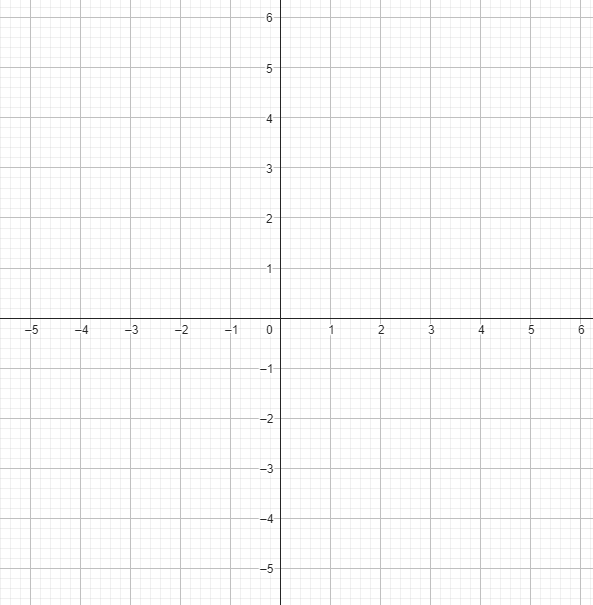
\includegraphics[width=\textwidth]{./imgSAEB_6_MAT/media/image39.png}
\end{figure}

A reta vertical é orientada para cima, e a reta horizontal é orientada
para a direita.

É comum usar as letras $x$ para a primeira e $y$ para a segunda, e os termos
``coordenada x'' e ``coordenada y''. Cada ponto sobre o plano é
representado por uma letra maiúscula.

Um polígono é uma figura geométrica plana formada por segmentos de reta
que se encontram apenas em suas extremidades. Um polígono é dito convexo
se qualquer segmento de reta que une dois pontos em seu interior estiver
completamente contido em seu interior.

Já um polígono é côncavo se existir pelo menos um segmento de reta que
une dois pontos em seu interior e que não está completamente contido em
seu interior. Em outras palavras, se houver algum ponto no interior do
polígono a partir do qual se possa traçar uma reta que corte uma aresta
do polígono.

\textbf{Fórmula de Euler}\\

\noindent A relação de Euler, quando aplicada a poliedros convexos, estabelece uma
relação fundamental entre o número de vértices ($V$), o número de arestas ($A$) e o
número de faces ($F$) desses poliedros. É dada pela seguinte expressão:

$$V - A + F = 2$$

\textbf{Elementos de circunferência}\\

\noindent Uma circunferência é uma figura geométrica plana formada por todos os
pontos que estão a uma distância constante, chamada raio, de um ponto
central. Os elementos de uma circunferência são:

\noindent\textit{Centro}\quad é o ponto central da circunferência, que fica equidistante de
todos os pontos da circunferência. O centro é geralmente representado
pela letra $O$.

\noindent\textit{Raio}\quad é a distância do centro até qualquer ponto da
circunferência. A letra $r$ é usada para representar o raio.

\noindent\textit{Diâmetro}\quad é uma reta que passa pelo centro da circunferência e que liga
dois pontos opostos da sua circunferência. O diâmetro é igual a duas
vezes o raio. A letra $d$ é usada para representar o diâmetro.

\noindent\textit{Corda}\quad é uma reta que liga dois pontos da circunferência. Uma corda não
necessariamente passa pelo centro da circunferência. Qualquer corda que
passe pelo centro é chamada de diâmetro.

\noindent\textit{Arco}\quad é uma parte da circunferência, limitada por dois pontos. O
comprimento do arco é proporcional ao ângulo central correspondente.}

\section*{Atividades}

\num{1}  Considere um poliedro convexo. Use a fórmula de Euler para determinar
o número de faces desse poliedro, sabendo que possui $10$ vértices e $20$
arestas.

\reduline{A fórmula de Euler para poliedros convexos é dada por $V - A + F = 2$.
Podemos usar essa fórmula para determinar o número de faces do poliedro
convexo com $V = 10$ e $A = 20$ da seguinte forma: $V - A + F = 2$; $10 - 20 + F = 2$; $F = 12$. Portanto, o número de faces do poliedro convexo é $12$.\hfill}

\num{2}  Uma professora resolveu lançar um desafio aos seus alunos. Deu
a eles várias coordenadas para colocarem em um plano
cartesiano:

\begin{myquote}
\begin{enumerate}
\item $A (0,5)$
\item $B (-1,2)$
\item $C (-4,2)$
\item $D (-2,0)$
\item $E (-3,-3)$
\item $F (0,1)$
\item $G (3,-3)$
\item $H (2,0)$
\item $I (4,2)$
\item $J (1,2)$
\end{enumerate}
\end{myquote}

Qual figura se formou ao ligar todos os pontos correspondentes?

\reduline{Ligando-se os pontos, obtém-se a figura de uma estrela.\hfill}
\linhas{1}

% \begin{figure}
% 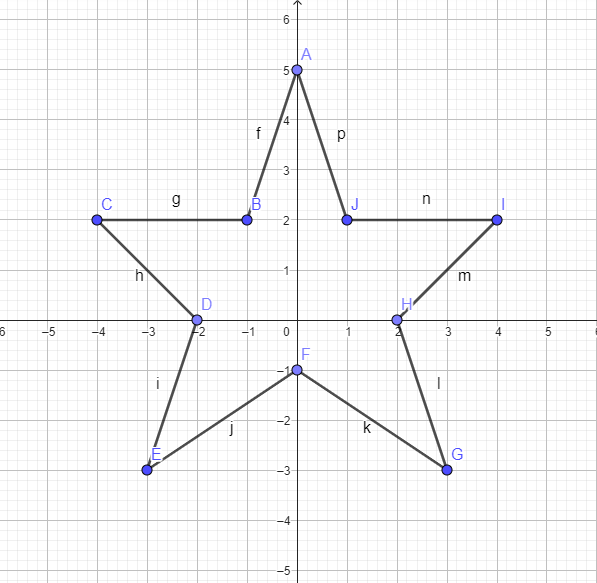
\includegraphics[width=3.85417in,height=3.56597in]{./imgSAEB_6_MAT/media/image45.png}
% \end{figure}

\num{3}  Para realizar o teste físico em determinado concurso da guarda
municipal, os candidatos devem correr ao redor de uma praça circular
cujo diâmetro mede $90$ m. Uma pessoa que dá $9$ voltas ao redor dessa praça
percorre quantos metros, se $\pi = 3$.

\begin{mdframed}[linewidth=2pt,linecolor=white,roundcorner=10pt]
\rosa{$2.430$ m.}
\vspace{6cm}
\end{mdframed}


\num{4}  Quantas arestas tem uma pirâmide quadrangular regular?

\reduline{
Uma pirâmide quadrangular regular tem uma base que é um quadrado, e
quatro faces triangulares congruentes que se encontram em um vértice
comum. Para contar o número de arestas da pirâmide, precisamos contar as
arestas da base (quatro) e as arestas que conectam o vértice da pirâmide
com os vértices da base (quatro). Portanto, a pirâmide quadrangular
regular tem $4 + 4 = 8$ arestas.\hfill}

\num{5}  Veja, a seguir, os diâmetros equatoriais dos planetas do sistema
solar.

\begin{myquote}
\begin{itemize}
  \item \textbf{Mercúrio}: 4.879,4 km;
  \item \textbf{Vênus}: 12.103,6 km;
  \item \textbf{Terra}: 12.756,2 km;
  \item \textbf{Marte}: 6.794,4 km;
  \item \textbf{Júpiter}: 142.984 km;
  \item \textbf{Saturno}: 120.536 km;
  \item \textbf{Urano}: 51.118 km;
  \item \textbf{Netuno}: 49.538 km.
\end{itemize}
\end{myquote}

Com base nesses números, calcule o raio de cada planeta.

\reduline{Mercúrio: 2.439,7 km. Vênus: 6.051,8 km. Terra: 6.378,1 km. Marte: 3.397,2 km. Júpiter: 71.492 km. Saturno: 60.268 km. Urano: 25.559 km. Netuno: 24.769 km.\hfill}
\linhas{3}

\num{6}  Qual é a medida do maior ângulo formado pelos ponteiros de um relógio
quando ele marca $9$ horas?

\reduline{$270$°.\hfill}

\num{7}  Se os ângulos internos de um polígono regular medem $36$°, então o
número de lados desse polígono é

\begin{escolha}
\item $10$. \rosa{X}
\item $17$.
\item $12$.
\item $13$.
\end{escolha}

\num{8}  Lourdes quer inovar em sua loja de cosméticos e decidiu embalar seus
produtos em caixas de diferentes formatos. Nas imagens a seguir estão as
planificações dessas caixas.

\begin{figure}[H]
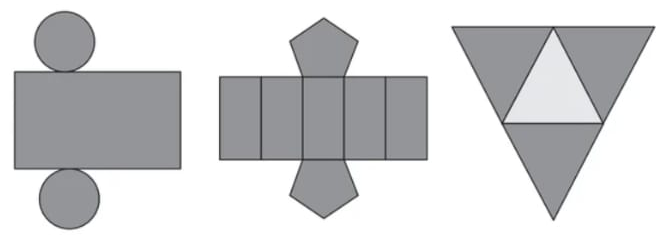
\includegraphics[width=5.90625in,height=2.125in]{./imgSAEB_6_MAT/media/image51.png}
\end{figure}

Quais serão os sólidos geométricos que Lourdes obterá a partir dessas
planificações?

\begin{escolha}
\item Cilindro, prisma de base pentagonal e pirâmide. \rosa{X}
\item Cone, prisma de base pentagonal e pirâmide.
\item Cone, tronco de pirâmide e pirâmide.
\item Cilindro, tronco de pirâmide e prisma.
\end{escolha}

\num{9}  Uma pista de atletismo tem a forma circular, e seu diâmetro mede $80$ m.
Um atleta treinando nessa pista deseja correr $10$ km diariamente.
Determine o número mínimo de voltas completas que ele deve dar nessa
pista a cada dia.

\rosa{Para determinar o número mínimo de voltas que o atleta deve dar na pista para cobrir uma distância de 10 km, primeiro, precisamos encontrar o comprimento da pista de atletismo, que é a circunferência do círculo.}

\rosa{A fórmula para calcular a circunferência de um círculo é dada por:}

\rosa{$\text{Circunferência} = \pi \times \text{Diâmetro}$}

\rosa{No caso da pista de atletismo, o diâmetro é 80 m. Portanto, a circunferência da pista é:}

\rosa{$\text{Circunferência} = \pi \times 80$}

\rosa{Para determinar o número de voltas necessárias para cobrir 10 km (10.000 m), dividimos a distância total pela circunferência da pista:}

\rosa{$\text{Número de Voltas} = \frac{10.000 \text{ m}}{\pi \times 80 \text{ m}}$}

\rosa{$\text{Número de Voltas} \approx \frac{10,000}{80 \times 3.1416} \approx \frac{10,000}{251.3274} \approx 39.8$}

\rosa{Como o atleta deve dar um número inteiro de voltas, ele precisará dar \(40\) voltas completas na pista para cobrir uma distância de 10 km diariamente.}

\num{10} A linha poligonal é conhecida por formar os polígonos e é de suma
importância nos estudos da geometria. Para ser identificado como um
polígono, o que uma figura geométrica plana precisa ser?

\reduline{A figura deve ser fechada e formada por segmentos de retas que não se cruzam.\hfill}
\linhas{2}

\section*{Treino}

\num{1}  Deseja-se pregar uma fita decorativa ao redor da tampa de um pote
redondo (sendo $\pi = 3$). Se o diâmetro da tampa mede $12$ cm, qual é o comprimento mínimo
que a fita deve ter para dar a volta completa nela?

\begin{escolha}
\item $72$ cm.
\item $108$ cm.
\item $35$ cm.
\item $11$ cm.
\end{escolha}

%\subsection{BNCC: EF06MA18 }
% -- Reconhecer, nomear e comparar polígonos, considerando
% lados, vértices e ângulos, e classificá-los em regulares e não
% regulares, tanto em suas representações no plano como em faces de
% poliedros.
% SAEB: Resolver problemas que envolvam relações entre os elementos de uma
% circunferência/círculo (raio, diâmetro, corda, arco, ângulo central,
% ângulo inscrito).

% Gabarito
% Alternativa A: incorreta, pois o aluno pode esquecer que o valor do raio
% é a metade do diâmetro, chegando nesse valor.
% Alternativa B: incorreta, pois ao confundir a fórmula do perímetro da
% circunferência com a fórmula da área da circunferência chegará a esse
% valor.
% Alternativa C: incorreta, pois, ao realizar uma soma ao invés de uma
% multiplicação na fórmula, obterá esse valor.
% Alternativa D: correta, pois ao considerar $\pi = 3$, temos que $2.3.6 = 36\,cm$.

\num{2}  Uma praça possui o formato circular com diâmetro medindo $20$ metros,
com $\pi = 3$.
Determine quantos metros quadrados de grama são necessários para preencher
essa área da praça.

\begin{multicols}{2}
\begin{escolha}
\item $300\,m^2$
\item $60\,m^2$
\item $1.200\,m^2$
\item $300\,cm^2$
\end{escolha}
\end{multicols}

%\subsection{BNCC: EF06MA18 }
% -- Reconhecer, nomear e comparar polígonos, considerando
% lados, vértices e ângulos, e classificá-los em regulares e não
% regulares, tanto em suas representações no plano como em faces de
% poliedros.
% SAEB: Resolver problemas que envolvam relações entre os elementos de uma
% circunferência/círculo (raio, diâmetro, corda, arco, ângulo central,
% ângulo inscrito).

% Gabarito
% Alternativa A: correta, pois, ao calcular a fórmula da área do círculo,
% temos que A= $3\times 10^2 = 300$m²
% Alternativa B: incorreta, pois, ao realizar o cálculo de perímetro da
% circunferência, ao invés do cálculo da área chegaremos a esse valor.
% Alternativa C: incorreta, pois o aluno pode esquecer de trocar o
% diâmetro pelo raio na fórmula e chegará a esse valor.
% Alternativa D: incorreta, pois o aluno pode esquecer de verificar que o
% valor do enunciado se trata de m² e não cm².

\num{3}  Num poliedro convexo, o número de faces é $6$ e o número de vértices é
$8$. Então, o número de arestas desse poliedro é

\begin{escolha}
\item $12$.

\item $14$.

\item $2$.

\item $48$.
\end{escolha}

%\subsection{BNCC: EF06MA17 }
% -- Quantificar e estabelecer relações entre o número de
% vértices, faces e arestas de prismas e pirâmides, em função do seu
% polígono da base, para resolver problemas e desenvolver a percepção
% espacial.
% SAEB: Relacionar o número de vértices, faces ou arestas de prismas ou
% pirâmides, em função do seu polígono da base.

% Gabarito
% Alternativa A: correta, pois $V + F = A + 2$; $8 + 6 = A + 2$; $14 = A + 2$; $A = 14 - 2$; $A = 12\,arestas$.
% Alternativa B: incorreta, pois o aluno pode somar todos os números do
% poliedro e chegar a essa conclusão equivocada.
% Alternativa C: incorreta pois o aluno pode realizar uma subtração ao
% invés de utilizar a fórmula.
% Alternativa D: incorreta o aluno pode realizar uma multiplicação ao
% invés de utilizar a fórmula.

\chapter{Triângulos}
\markboth{Módulo 8}{}

\section*{Habilidades do SAEB} 
\begin{itemize}
\item Identificar propriedades e relações existentes
entre os elementos de um triângulo (condição de existência, relações de
ordem entre as medidas dos lados e as medidas dos ângulos internos, soma
dos ângulos internos, determinação da medida de um ângulo interno ou
externo).
\item
  Classificar triângulos ou quadriláteros em relação aos lados ou aos
  ângulos internos.
\item
  Identificar retas ou segmentos de retas concorrentes, paralelos ou
  perpendiculares.
\item
  Identificar relações entre ângulos formados por retas paralelas
  cortadas por uma transversal.
\item
  Resolver problemas que envolvam relações entre ângulos formados por
  retas paralelas cortadas por uma transversal, ângulos internos ou
  externos de polígonos ou cevianas (altura, bissetriz, mediana,
  mediatriz) de polígonos.
\item
  Resolver problemas que envolvam relações métricas do triângulo
  retângulo, incluindo o teorema de Pitágoras.
\item
  Resolver problemas que envolvam polígonos semelhantes.
\item
  Resolver problemas que envolvam aplicação das relações de
  proporcionalidade abrangendo retas paralelas cortadas por
  transversais.
\item
  Determinar o ponto médio de um segmento de reta ou a distância entre
  dois pontos quaisquer, dadas as coordenadas desses pontos no plano
  cartesiano.
\end{itemize}

\subsection{Habilidade da BNCC} 

\begin{itemize}
\item EF06MA19.
\end{itemize}

\conteudo{
\noindent Existem vários tipos de triângulo, e eles podem ser classificados de
acordo com seus lados e ângulos. Veja os principais tipos de triângulo:

\begin{itemize}
\item\textit{Triângulo equilátero}. Um triângulo equilátero é aquele em que todos os
três lados são iguais. Além disso, todos os ângulos internos desse tipo
de triângulo são iguais a $60$ graus.
\item\textit{Triângulo isósceles}. Um triângulo isósceles tem dois lados iguais e um
lado diferente. Os dois ângulos formados pelos lados iguais são iguais
entre si, enquanto o terceiro ângulo é diferente.
\item\textit{Triângulo escaleno}. Um triângulo escaleno é aquele em que todos os três
lados são diferentes. Como resultado, os três ângulos internos também
são diferentes.
\item\textit{Triângulo retângulo}. Um triângulo retângulo tem um ângulo reto (isto é,
um ângulo de $90$ graus). O lado oposto ao ângulo reto é chamado de
hipotenusa, enquanto os outros dois lados são chamados de catetos. O
teorema de Pitágoras é frequentemente usado para resolver problemas que
envolvem triângulos retângulos.
\item\textit{Triângulo obtusângulo}. Um triângulo obtusângulo é aquele em que um dos
ângulos internos é obtuso, ou seja, tem mais de $90$ graus.
\item\textit{Triângulo acutângulo}. Um triângulo acutângulo é aquele em que todos os
ângulos internos são agudos, ou seja, têm menos de $90$ graus.
\end{itemize}}

\section*{Atividades}

\num{1} Maria está desenhando triângulos para um projeto de arte na escola.
Ela tem três segmentos de reta de diferentes comprimentos: $5$ cm, $8$ cm e $10$ cm.
Ela quer saber se é possível formar um triângulo usando esses segmentos de reta.
Além disso, ela gostaria de saber que tipo de triângulo seria, se possível.
Escreva um texto explicativo para Maria, ajudando-a a entender se é possível
formar um triângulo com esses segmentos de reta e, caso seja possível, explique que
tipo de triângulo seria formado com base nas medidas dadas.

\reduline{Para determinar se é possível formar um triângulo com os segmentos de reta dados,
precisamos aplicar a condição de existência de um triângulo, que é a seguinte:
a soma de dois lados de um triângulo deve ser sempre maior do que o terceiro lado.
Vamos verificar isso com os segmentos de 5 cm, 8 cm e 10 cm:

- 5 cm + 8 cm = 13 cm (maior que 10 cm);
- 5 cm + 10 cm = 15 cm (maior que 8 cm);
- 8 cm + 10 cm = 18 cm (maior que 5 cm).

Como a soma de cada par de segmentos é maior do que o terceiro segmento,
é possível formar um triângulo com esses comprimentos.

Além disso, um triângulo com lados de comprimentos 5 cm, 8 cm e 10 cm é classificado como um triângulo escaleno.
Triângulos escalenos são triângulos que têm todos os lados com comprimentos diferentes.}

\num{2} O que é ponto médio?

\reduline{É o ponto central entre dois outros pontos.\hfill}

\num{3} Com base no mapa a seguir, marque V para o que for verdadeiro e F para o que for falso.

\begin{figure}[H]
\centering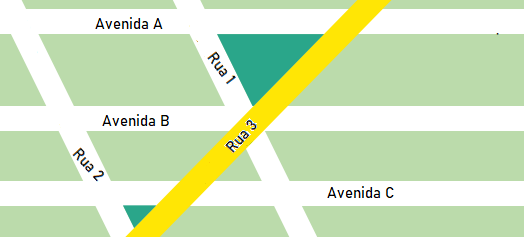
\includegraphics[width=5.47917in,height=2.48958in]{./imgSAEB_6_MAT/media/image53.png}
\end{figure}

\begin{boxlist}
\boxitem{V} As avenidas A e B são paralelas entre si.
\boxitem{F} Pode se considerar que a Rua 2 é paralela à avenida C.
\boxitem{F} A avenida C não é paralela à Avenida B.
\boxitem{V} As ruas 2 e 3 são concorrentes entre si.
\boxitem{V} A Rua 1 e a Rua 3 não são paralelas entre si.
\boxitem{F} A Rua 1 e a Rua 2 são concorrentes entre si.
\end{boxlist}

\num{4}  Angélica decidiu pintar um quadro com as seguintes dimensões: $100\,cm$ de largura
por $85\,cm$ de altura, com $3$ esferas de cores diferentes. Observe a imagem a seguir.

\begin{figure}[H]
\centering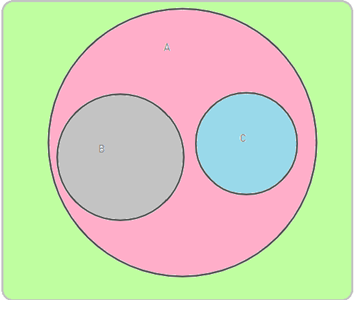
\includegraphics[width=3.70833in,height=3.22917in]{./imgSAEB_6_MAT/media/image54.png}
\end{figure}

Qual é a área
pintada de cada parte do quadro sabendo que a esfera A tem $60\,cm$ de
diâmetro, a esfera B $20\,cm$ de diâmetro, e a esfera C, $10\,cm$ de diâmetro. Considere $\pi = 3$.

\begin{multicols}{2}
\begin{escolha}
\item Área cinza.

\reduline{$1.200\,cm^2$.\hfill}
\item área azul.

\reduline{$75\,cm^2$.\hfill}
\item Área rosa.

\reduline{$2.700\,cm^2$.\hfill}
\item Área verde.

\reduline{$4.525\,cm^2$.\hfill}
\end{escolha}
\end{multicols}

\begin{mdframed}[linewidth=2pt,linecolor=white,roundcorner=10pt]
\vspace{6cm}
\end{mdframed}

\num{5}  Calcule a diagonal de um retângulo de lados $8\,cm$ e $15\,cm$.

% \begin{figure}[h]
% \centering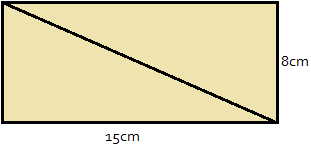
\includegraphics[width=3.24444in,height=1.54653in]{./imgSAEB_6_MAT/media/image55.png}
% \end{figure}

\rosa{$A^2 = B^2+ C^2$}

\rosa{$A^2 = 8^2 + 15^2$}

\rosa{$A^2 = 64 + 225$}

\rosa{$A^2 = 289$}

\rosa{$A = 17\,cm^2$}

\num{6}  Um fazendeiro quer construir uma cerca para seu campo, que tem a
forma de um triângulo retângulo. Ele sabe que a distância entre os dois
pontos mais distantes do campo é de $50$ metros e que a distância entre
esses pontos e um terceiro ponto no campo é de $30$ metros. Qual é o
comprimento total da cerca que o fazendeiro precisa comprar?

\rosa{Vamos considerar o triângulo retângulo $ABC$, em que $AB$ é a hipotenusa, $AC$ é um dos catetos com comprimento 50 metros e $BC$ é o outro cateto, com comprimento 30 metros.}

\rosa{Vamos considerar um triângulo retângulo $ADC$, em que $AD$ representa a distância entre os pontos mais distantes do campo (50 metros) e $CD$ representa a distância do terceiro ponto até a linha em que o fazendeiro quer construir a cerca (30 metros).}

\rosa{Os triângulos $ABC$ e $ADC$ são semelhantes porque têm um ângulo comum ($\angle ADC$ e $\angle ABC$) e um ângulo reto ($\angle DAC$ e $\angle CAB$).}

\rosa{Pela propriedade dos triângulos semelhantes, sabemos que os lados correspondentes desses triângulos estão na mesma razão. Portanto, podemos escrever a seguinte proporção:}

\rosa{$\frac{AB}{AC} = \frac{AD}{CD}$}

\rosa{$\frac{AB}{50} = \frac{50}{30}$}

\rosa{$AB = \frac{50 \times 50}{30} = \frac{2.500}{30} \approx 83,33$}

\rosa{O fazendeiro precisa comprar, aproximadamente, $83,33$ metros de cerca para cercar seu campo.}

\num{7}  Um triângulo tem um ângulo interno de $90$ graus, e seus outros dois
ângulos internos são iguais entre si. Além disso, o comprimento de um
dos lados desse triângulo é o dobro do comprimento do outro lado.
Determine os tipos de triângulo possíveis que satisfazem a essas
condições.

\reduline{o triângulo pode ser um triângulo retângulo isósceles ou um triângulo
retângulo escaleno.\hfill}
\linhas{1}

\num{8}  Um triângulo tem dois lados iguais, cada um medindo $6\,cm$,
e um ângulo diferente, medindo $45$ graus. Classifique esse triângulo de
acordo com seus lados e ângulos.

\reduline{Podemos classificar esse triângulo de duas maneiras: por seus lados
ou por seus ângulos. Pelos lados, esse triângulo tem dois lados iguais, o que significa que é um triângulo isósceles. Pelos ângulos, podemos usar a soma dos ângulos internos de um triângulo,
que é sempre igual a $180$ graus, para encontrar o valor do terceiro
ângulo. Como dois ângulos são iguais a $45$ graus cada, a soma desses
ângulos é $90$ graus. Portanto, o terceiro ângulo é: $180 - 90 = 90$ graus. Esse é um ângulo reto, o que significa que esse triângulo é também um
triângulo retângulo. Assim, podemos concluir que esse triângulo é um triângulo isósceles e
retângulo.\hfill}

\num{9} Um prédio tem $25$ metros de altura, e um poste de luz de $10$ metros de
altura está a certa distância da base do prédio. A distância entre a
base do prédio e a base do poste de luz é de $20$ metros. Qual é a
distância entre o topo do poste de luz e o topo do prédio?

\rosa{Vamos nomear os pontos:}

\rosa{- A base do prédio: $P$.}

\rosa{- O topo do prédio: $Q$.}

\rosa{- A base do poste de luz: $R$.}

\rosa{- O topo do poste de luz: $S$.}

\rosa{Sabemos que a altura do prédio ($AP$) é de $25$ metros, a altura do poste de luz ($BR$) é de $10$ metros, e a distância entre a base do prédio e a base do poste de luz ($PR$) é de $20$ metros.}

\rosa{Os triângulos $PQR$ e $QPS$ são semelhantes, pois ambos têm um ângulo reto (devido à verticalidade) e compartilham um ângulo comum, ($\angle Q$). Portanto, podemos estabelecer a seguinte proporção:}

\rosa{$\frac{QR}{PR} = \frac{PS}{PQ}$}

\rosa{$\frac{10}{20} = \frac{PS}{25}$}

\rosa{$PS = 12,5$} metros

\rosa{Para encontrar a distância entre o topo do poste de luz ($S$) e o topo do prédio ($Q$), podemos usar a diferença entre as alturas:}

\rosa{$QS = PQ - PS = 25 - 12.5 = 12.5 \text{ metros}$}

\rosa{A distância entre o topo do poste de luz e o topo do prédio é de $12,5$ metros.}

\num{10} Um arquiteto está projetando uma nova praça em um terreno retangular.
A praça tem um formato triangular, com um dos lados paralelo à borda do terreno.
Esse lado triangular mede $15$ metros. O arquiteto precisa determinar o comprimento
do lado inclinado do triângulo, bem como os ângulos internos do triângulo.
Como o arquiteto pode determinar o comprimento do lado inclinado?
Além disso, como ele pode calcular os ângulos internos do triângulo?

\reduline{Para determinar o comprimento do lado inclinado do triângulo sem usar o Teorema de Pitágoras ou funções trigonométricas, podemos usar o Teorema de Tales, segundo o qual, se duas retas paralelas cortam transversais em pontos distintos, então essas transversais dividem as retas em segmentos proporcionais. Nesse caso, podemos considerar o lado inclinado do triângulo como uma transversal cortando duas retas paralelas (um lado do terreno e o solo). Se o lado paralelo ao terreno mede $15$ metros, e o terreno forma um retângulo, então o arquiteto pode dividir esse lado em segmentos proporcionais para encontrar o comprimento do lado inclinado. Para calcular os ângulos internos do triângulo, podemos usar a soma dos ângulos internos de um triângulo, que sempre totaliza $180^\circ$. Se conhecemos dois ângulos do triângulo (um ângulo reto formado pela base do terreno e o solo, e outro ângulo formado pelo lado inclinado e o solo), podemos encontrar o terceiro ângulo subtraindo a soma dos ângulos conhecidos de $180^\circ$. Dessa forma, podemos determinar todos os ângulos internos do triângulo sem o uso de funções trigonométricas.}

\section*{Treino}

\num{1}  Sabendo que $OP$ é bissetriz do ângulo $AÔB$, qual é o valor de $x$?

\begin{figure}[H]
\centering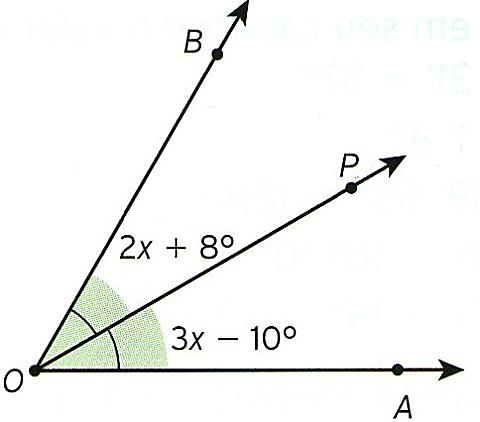
\includegraphics[width=2.17708in,height=1.91619in]{./imgSAEB_6_MAT/media/image62.jpeg}
\end{figure}

\begin{escolha}
\item $-2,5$.
\item $13$.
\item $18$.
\item $45$.
\end{escolha}

%\subsection{BNCC: EF06MA19}
%  -- Identificar características dos triângulos e
% classificá-los em relação às medidas dos lados e dos ângulos.
% SAEB: Identificar relações entre ângulos formados por retas paralelas
% cortadas por uma transversal.

% Gabarito
% Alternativa A: incorreta, pois o aluno pode chegar a essa conclusão
% somando os valores literais e dividindo em seguida pelos números
% restantes.
% Alternativa B: incorreta, pois o aluno pode considerar multiplicar os
% valores e dividir após o resultado para chegar a esse valor.
% Alternativa C: correta, pois, Utilizando os conhecimentos sobre
% bissetriz obtemos que as medidas dos Ângulos BÔP e PÔA são iguais, logo $2x+8=3x-10$; $2x-3x= -10 - 8$; $-x = -18$; $x = 18$.
% Alternativa D: incorreta, pois o aluno, pela falta de conhecimento sobre
% bissetriz, pode relembrar que $45$ seja o valor da bissetriz do ângulo
% reto e chegar a essa conclusão mesmo não se tratando de um ângulo reto.

\num{2}  Em um triângulo, se um ângulo mede $90$ graus, quanto mede a soma dos
outros dois ângulos?

\begin{escolha}
\item $60$ graus.
\item $90$ graus.
\item $100$ graus.
\item $180$ graus.
\end{escolha}

%\subsection{BNCC: EF06MA19 }
% -- Identificar características dos triângulos e
% classificá-los em relação às medidas dos lados e dos ângulos.
% SAEB: Identificar relações entre ângulos formados por retas paralelas
% cortadas por uma transversal.

% Gabarito
% Alternativa A: incorreta, pois o aluno errou na soma dos ângulos.
% Alternativa B: incorreta, pois o aluno não soube aplicar a soma dos
% ângulos internos.
% Alternativa C: incorreta, pois o aluno não somou $80$º para encontrar o
% resultado correto.
% Alternativa D: correta, pois a soma dos ângulos internos de um triângulo
% é sempre igual a $180$ graus. Se um dos ângulos mede $90$ graus, a soma dos
% outros dois ângulos deve ser igual a $180 - 90 = 90$ graus.

\num{3}  Francisco resolveu fazer um brinquedo de madeira em formato de um
triangulo equilátero para seu filho brincar. Sendo assim, comprou $3$ peças
de madeira com medidas diferentes, $50\,cm$, $60\,cm$ e $70\,cm$, para que ele
corte apenas $2$ peças. Qual é a medida que os lados do triangulo
necessariamente devem ter?

\begin{escolha}
\item $70\,cm$.
\item $25\,cm$.
\item $50\,cm$.
\item $55\,cm$.
\end{escolha}

%\subsection{BNCC: EF06MA19 }
% -- Identificar características dos triângulos e
% classificá-los em relação às medidas dos lados e dos ângulos.
% SAEB: Identificar relações entre ângulos formados por retas paralelas
% cortadas por uma transversal.

% Gabarito
% Alternativa A: incorreta, pois o aluno pode considerar cortar mais peças
% em relação àquilo que o enunciado recomenda.
% Alternativa B: incorreta, pois o aluno pode considerar cortar mais peças
% em relação àquilo que o enunciado recomenda.
% Alternativa C: correta, pois, para cortar apenas $2$ peças de madeira, o
% brinquedo deverá ser um triangulo de lado $50\,cm$. Como será um triangulo
% equilátero, terá $3$ lados iguais.
% Alternativa D: incorreta, pois o aluno pode considerar cortar mais peças
% em relação àquilo que o enunciado recomenda.

\chapter{A representação do espaço}
\markboth{Módulo 9}{}

\section*{Habilidade do SAEB} 
\begin{itemize}
\item Descrever ou esboçar deslocamento de pessoas e/ou
ento de pessoas e/ou de objetos em representações bidimensionais (mapas, croquis etc.),
plantas de ambientes ou vistas, de acordo com condições dadas.
\end{itemize}

\subsection{Habilidade da BNCC} 
\begin{itemize}
\item EF06MA21.
\end{itemize}

\conteudo{O espaço pode ser representado de diferentes maneiras.

\noindent\textbf{Mapa}\quad é uma representação gráfica e simbólica de uma região ou área,
geralmente em escala reduzida, que apresenta informações sobre a
localização, a topografia, a hidrografia, a vegetação e a infraestrutura,
entre outros elementos geográficos ou culturais.

\noindent\textbf{Planta}\quad é um tipo de mapa que representa a planta baixa ou a vista aérea
de uma construção, um edifício, uma casa, um jardim ou um terreno, por exemplo. É
utilizada na arquitetura, na engenharia civil, no urbanismo e no paisagismo,
entre outras áreas.

\noindent\textbf{Croqui}\quad é um desenho esquemático, geralmente feito a mão livre, que
representa um objeto, uma paisagem, um ambiente ou uma ideia de forma
simplificada e sem escala. É usado em diversos campos, como arquitetura,
\textit{design}, geografia, artes, entre outros.

A \textbf{escala}\quad é a relação matemática entre as medidas reais e as medidas
representadas em mapa, planta ou croqui. Ela indica quantas vezes a
distância real é maior do que a distância representada no desenho. Por
exemplo, uma escala de $1:1.000$ significa que cada $1\,cm$ no mapa representa
$1,000\,cm$ (ou $10$ metros) na realidade. A escala é fundamental para
garantir a precisão e a confiabilidade das informações apresentadas em
uma representação desses tipos.}

\section*{Atividades}

\num{1}  Veja a seguir o mapa do entrno do local onde José mora.

\begin{figure}[H]
\centering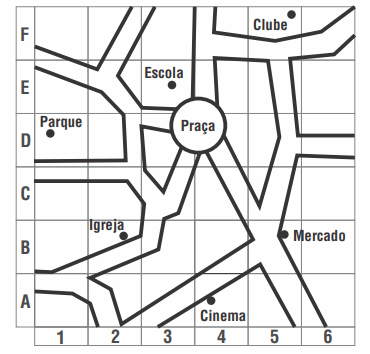
\includegraphics[width=3.86042in,height=3.68611in]{./imgSAEB_6_MAT/media/image64.png}
\end{figure}

No mapa, José quer localizar a escola considerando um número e uma letra.
Qual é a localização da escola?

\reduline{E3.\hfill}

\num{2}  Observe a seguir a representação de parte do mapa de uma cidade
planejada.

\begin{figure}[H]
\centering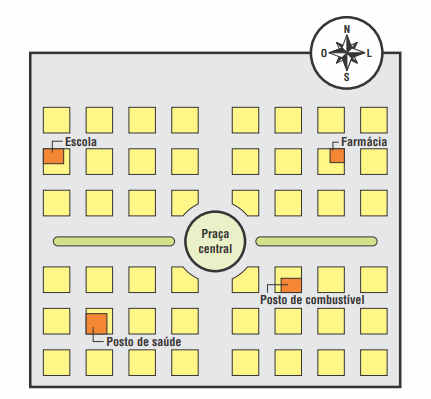
\includegraphics[width=3.39535in,height=3.14326in]{./imgSAEB_6_MAT/media/image65.png}
\end{figure}

Juca saiu da praça central e, orientando-se por esse mapa, caminhou $3$
quadras na direção leste e depois $2$ quadras na direção norte. Diante disso,
determine o local em que Juca parou.

\reduline{Juca parou no posto de gasolina.\hfill}
\linhas{1}

\num{3}  Observe a seguir o mapa do bairro onde Gabriela mora.

\begin{figure}[H]
\centering
\includegraphics[width=4.95347in,height=3.13958in]{./imgSAEB_6_MAT/media/image66.png}
\end{figure}

Gabriela estava na Praça dos Coqueiros e passou na padaria antes de ir
para casa. Qual dos caminhos Gabriela fez para chegar a sua casa?

\reduline{Gabriela entrou na Rua das Margaridas e virou na Rua dos Cravos.\hfill}
\linhas{2}

\num{4}  O croqui a seguir mostra um mapa que fornece as indicações para se
chegar a uma chácara.

\begin{figure}[H]
\centering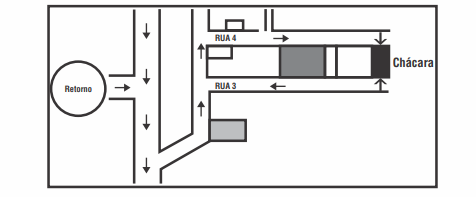
\includegraphics[width=4.95347in,height=2.04653in]{./imgSAEB_6_MAT/media/image67.png}
\end{figure}

O que Luna deve fazer, para chegar à chácara, após fazer o retorno?

\reduline{Virar à direita, virar à esquerda e entrar na Rua 4.\hfill}
\linhas{2}

\num{5}  Observe o mapa a seguir.

\begin{figure}[H]
\centering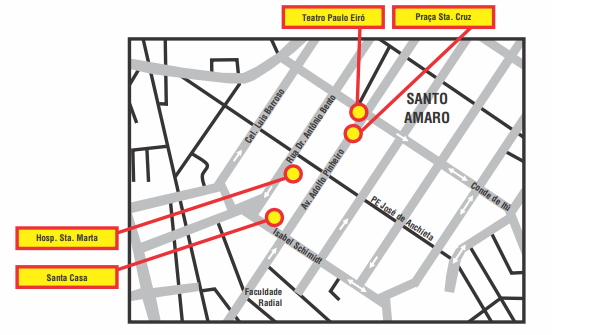
\includegraphics[width=5.90625in,height=3.34375in]{./imgSAEB_6_MAT/media/image68.png}
\end{figure}

O que está localizado na Rua Isabel Schimdt, entre a Rua Dr. Antônio Bento e a Avenida
Adolfo Pinheiro?

\reduline{Está localizada a Santa Casa.\hfill}

\num{6}  A figura a seguir representa a localização de quatro crianças em relação às
ruas Alegria e Beija-Flor. As demais ruas traçadas são paralelas à Rua
Alegria ou à Rua Beija-flor. Observe.

\begin{figure}[H]
\centering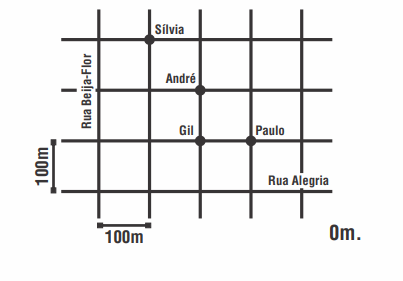
\includegraphics[width=4.19792in,height=2.93056in]{./imgSAEB_6_MAT/media/image69.png}
\end{figure}

Que criança está à mesma distância das duas ruas?

\begin{boxlist}
\boxitem{\white{X}} Sílvia.
\boxitem{\rosa{X}} André.
\boxitem{\white{X}} Gil.
\boxitem{\white{X}} Paulo.
\end{boxlist}

% \num{7}  Observe o mapa abaixo. Segundo o Mapa, a Praça da Matriz e o Hospital São José se localizam,
% respectivamente, nas coordenadas:

% \begin{figure}[h]
% \centering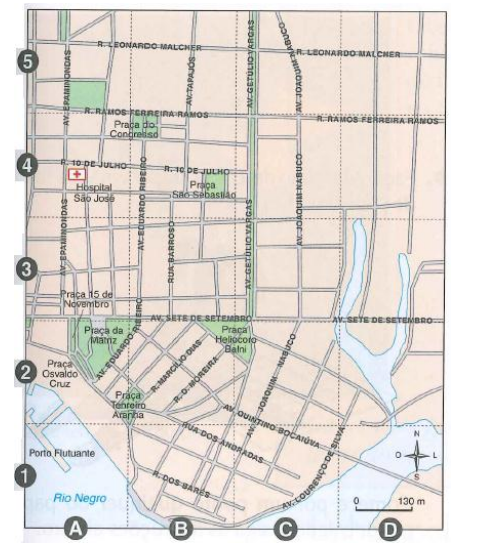
\includegraphics[width=5.08333in,height=5.71875in]{./imgSAEB_6_MAT/media/image70.png}
% \end{figure}

% \reduline{(A, $2$) e (A, $4$).\hfill}

\num{7}  Hélio desenhou a planta da casa onde mora. Ela tem dois quartos, uma
sala, uma cozinha e um banheiro.

\begin{figure}[H]
\centering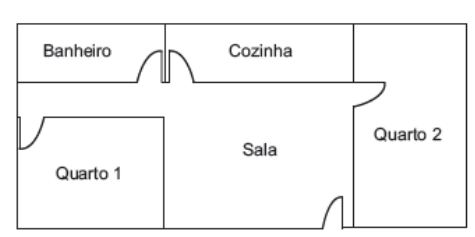
\includegraphics[width=4.94792in,height=2.46875in]{./imgSAEB_6_MAT/media/image71.png}
\end{figure}

Ao entrar em sua casa pela porta da sala e virar à direita, Hélio está
indo em direção a que cômodo da casa?

\reduline{Nesse caso, ele está indo em direção ao quarto 2.\hfill}
\linhas{1}

\num{8}  A figura a seguir representa o mapa de um bairro, sendo que cada
quadrado representa um quarteirão, cuja distância entre duas esquinas é
de $100$ m.

\begin{figure}[H]
\centering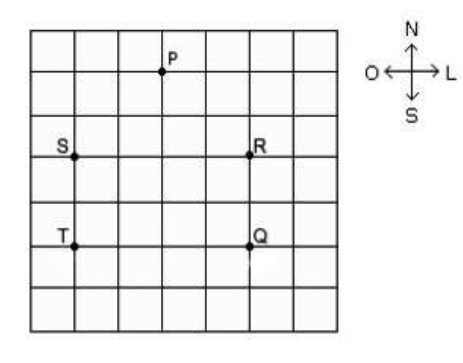
\includegraphics[width=4.82569in,height=3.77917in]{./imgSAEB_6_MAT/media/image72.png}
\end{figure}

Uma pessoa saiu da esquina indicada pelo ponto P e percorreu o seguinte
percurso:

\begin{itemize}
\item Caminhou $300$ metros na direção Sul;
\item Caminhou $200$ metros na direção Leste;
\item Caminhou $100$ metros na direção Sul.
\end{itemize}

Ao final desse percurso, essa pessoa chegou à esquina indicada por qual letra?

\reduline{A letra Q representa a esquina a que essa pessoa chegou.\hfill}

\num{9} Bia e Celso estão jogando batalha naval. Em dado momento, só sobrou
um submarino para Bia, na posição descrita na figura a seguir.

\begin{figure}[H]
\centering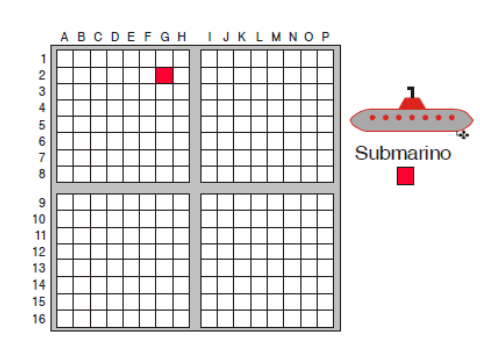
\includegraphics[width=5in,height=3.55208in]{./imgSAEB_6_MAT/media/image73.png}
\end{figure}

Em que ponto do mapa da batalha naval Celso deve atacar para vencer o jogo?

\reduline{Ele deve atacar no ponto G2.\hfill}

\section*{Treino}

\num{1}  Na imagem a seguir, os retângulos representam cidades. Os números
representam os preços (em reais) dos bilhetes do tranporte entre cidades vizinhas. Observe.

\begin{figure}[H]
\centering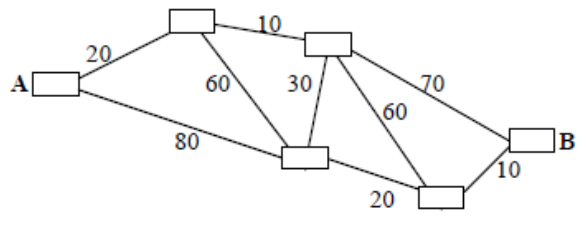
\includegraphics[width=5.90625in,height=2.38542in]{./imgSAEB_6_MAT/media/image74.png}
\end{figure}

Evandro quer ir da cidade A para a cidade B usando o trajeto mais
barato.
Qual é o menor preço que ele deve pagar?

\begin{escolha}
\item R\$ 80,00.
\item R\$ 90,00.
\item R\$ 100,00.
\item R\$ 110,00.
\end{escolha}

%\subsection{BNCC: EF06MA21 }
% -- Construir figuras planas semelhantes em situações de
% ampliação e de redução, com o uso de malhas quadriculadas, plano
% cartesiano ou tecnologias digitais.
% SAEB: Descrever ou esboçar deslocamento de pessoas e/ou de objetos em
% representações bidimensionais (mapas, croquis etc.), plantas de
% ambientes ou vistas, de acordo com condições dadas

% Gabarito
% Alternativa A: incorreta, pois o aluno pode esquecer de somar um
% quadrinho e chegar a esse número.
% Alternativa B: correta: pois, é utilizada a rota $20 + 10 + 30 + 20 + 10 = 90$.
% Alternativa C: incorreta, pois o aluno pode considerar seguir por uma
% rota que não seja a mais vantajosa.
% Alternativa D: incorreta, pois o aluno pode considerar seguir por uma
% rota que não seja a mais vantajosa.

\num{2} No mapa a seguir, encontram-se representadas as ruas do bairro onde
Natasha mora. Natasha informou que mora numa rua entre as avenidas A e B e entre as
ruas do hospital e da locadora.

\begin{figure}[H]
\centering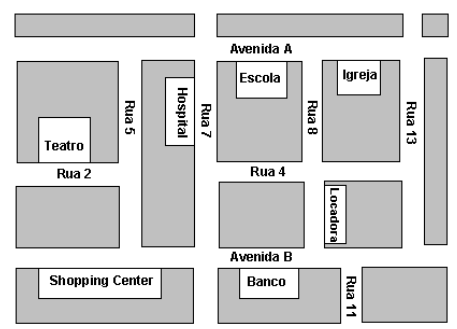
\includegraphics[width=4.76042in,height=3.42708in]{./imgSAEB_6_MAT/media/image75.png}
\end{figure}

Ela mora na rua

\begin{multicols}{2}
\begin{escolha}
\item 4.
\item 5.
\item 7.
\item 9.
\end{escolha}
\end{multicols}

%\subsection{BNCC: EF06MA21 }
% -- Construir figuras planas semelhantes em situações de
% ampliação e de redução, com o uso de malhas quadriculadas, plano
% cartesiano ou tecnologias digitais.
% SAEB: Descrever ou esboçar deslocamento de pessoas e/ou de objetos em
% representações bidimensionais (mapas, croquis etc.), plantas de
% ambientes ou vistas, de acordo com condições dadas

% Gabarito
% Alternativa A: correta, pois as coordenadas indicam essa localização.
% Alternativa B: incorreta, pois o aluno pode se perder na condução do
% mapa e chegar a essa conclusão erroneamente.
% Alternativa C: incorreta, pois o aluno pode se perder na condução do
% mapa e chegar a essa conclusão erroneamente.
% Alternativa D: incorreta, pois o aluno pode se perder na condução do
% mapa e chegar a essa conclusão erroneamente.

\num{3}  Qual das seguintes afirmações melhor descreve a diferença entre mapa,
planta e croqui?

\begin{escolha}
\item
  Um mapa é uma representação de uma região ou área, enquanto uma planta
  é um desenho esquemático de uma construção, e um croqui é uma vista
  aérea de uma cidade ou paisagem.
\item
  Um mapa é uma vista aérea de uma cidade ou paisagem, enquanto uma
  planta é uma representação de uma região ou área, e um croqui é um
  desenho esquemático de uma construção.
\item
  Um mapa é um desenho esquemático de uma construção, enquanto uma
  planta é uma representação de uma região ou área, e um croqui é uma
  vista aérea de uma cidade ou paisagem.
\item
  Um mapa, uma planta e um croqui são todos sinônimos e podem ser usados
  de forma intercambiável.
\end{escolha}


%\subsection{BNCC: EF06MA21 }
% -- Construir figuras planas semelhantes em situações de
% ampliação e de redução, com o uso de malhas quadriculadas, plano
% cartesiano ou tecnologias digitais.
% SAEB: Descrever ou esboçar deslocamento de pessoas e/ou de objetos em
% representações bidimensionais (mapas, croquis etc.), plantas de
% ambientes ou vistas, de acordo com condições dadas

% Gabarito
% Alternativa A: correta, pois essa definição está correta.
% Alternativa B: incorreta, pois as primeiras definições estão incorretas.
% Alternativa C: incorreta, pois a definição de planta está incorreta.
% Alternativa D: incorreta, pois há diferenças entre esses conceitos.

\chapter{A leitura de gráficos}
\markboth{Módulo 10}{}

\section*{Habilidades do SAEB} 
\begin{itemize}
\item Identificar os indivíduos (universo ou
população-alvo da pesquisa), as variáveis e os tipos de variáveis
(quantitativas ou categóricas) em um conjunto de dados.
\item
  Representar ou associar os dados de uma pesquisa estatística ou de um
  levantamento em listas, tabelas (simples ou de dupla entrada) ou
  gráficos (barras simples ou agrupadas, colunas simples ou agrupadas,
  pictóricos, de linhas, de setores, ou em histograma).
\item
  Inferir a finalidade da realização de uma pesquisa estatística ou de
  um levantamento, dada uma tabela (simples ou de dupla entrada) ou
  gráfico (barras simples ou agrupadas, colunas simples ou agrupadas,
  pictóricos, de linhas, de setores ou em histograma) com os dados dessa
  pesquisa. - Interpretar o significado das medidas de tendência central
  (média aritmética simples, moda e mediana) ou da amplitude.
\item
  Calcular os valores de medidas de tendência central de uma pesquisa
  estatística (média aritmética simples, moda ou mediana).
\item
  Resolver problemas que envolvam dados estatísticos apresentados em
  tabelas (simples ou de dupla entrada) ou gráficos (barras simples ou
  agrupadas, colunas simples ou agrupadas, pictóricos, de linhas, de
  setores ou em histograma).
\item
  Argumentar ou analisar argumentações/conclusões com base nos dados
  apresentados em tabelas (simples ou de dupla entrada) ou gráficos
  (barras simples ou agrupadas, colunas simples ou agrupadas,
  pictóricos, de linhas, de setores ou em histograma).
\item
  Explicar/descrever os passos para a realização de uma pesquisa
  estatística ou de um levantamento.
\end{itemize}

\subsection{Habilidades da BNCC}
\begin{itemize} 
\item EF06MA31, EF06MA32.
\end{itemize}


\conteudo{Na vastidão do conhecimento humano, a estatística representa uma ferramenta
poderosa para entender o mundo ao nosso redor. Numéricos e objetivos, os dados
são como peças de um quebra-cabeça complexo, cada uma contendo informações
valiosas. Nesta jornada intelectual, mergulharemos nas profundezas dos dados e
exploraremos as habilidades fundamentais associadas à estatística.

\begin{figure}[H]
\centering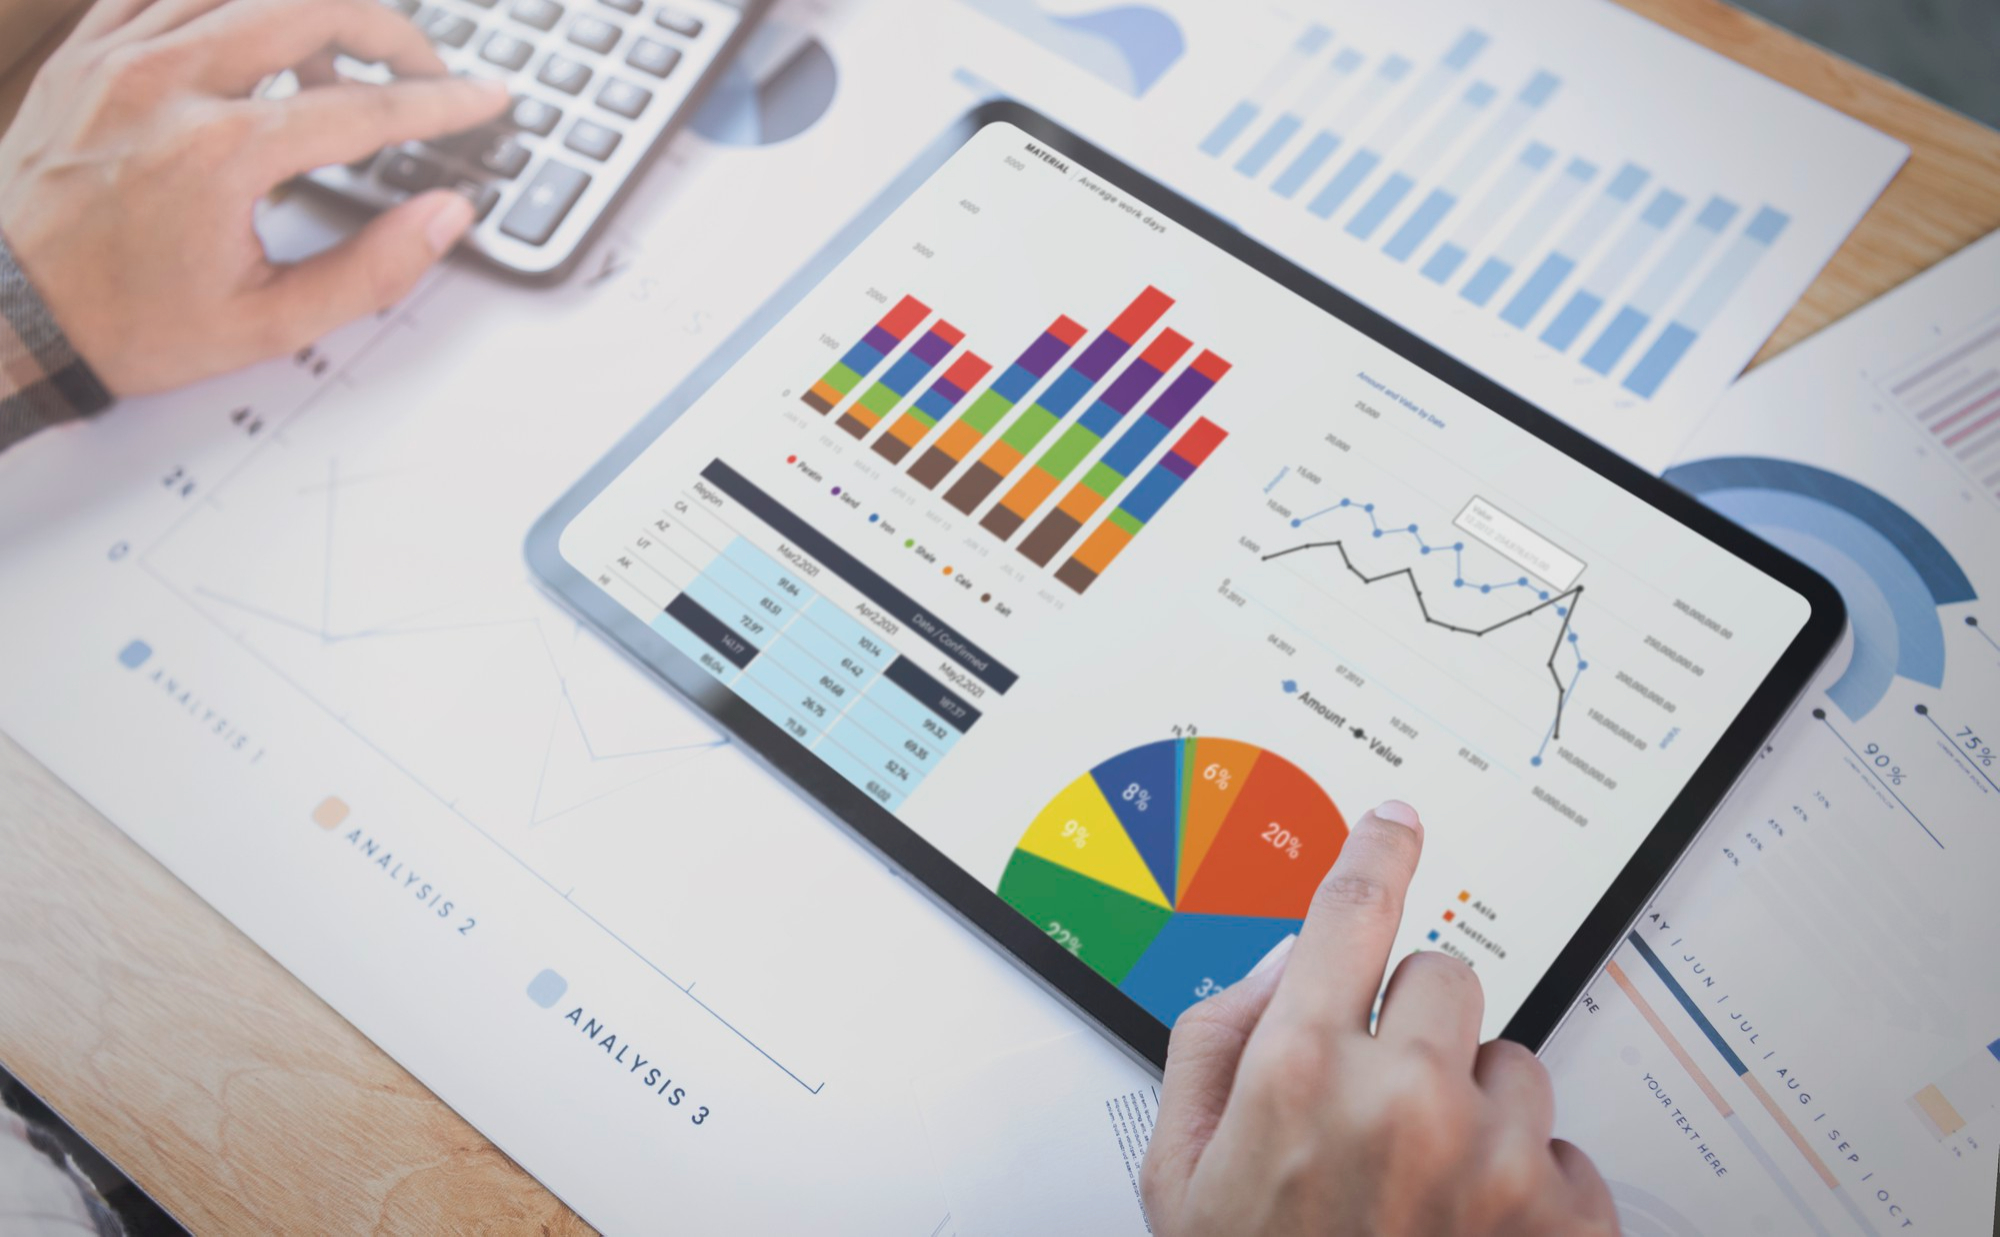
\includegraphics[width=3.92708in,height=0.8125in]{./imgSAEB_6_MAT/media/image134.png}
\end{figure}

Para iniciar nossa exploração, é crucial compreender três elementos cruciais:
os \textbf{indivíduos}, as \textbf{variáveis} e os \textbf{tipos de variável}. Imagine um conjunto de
dados como um mapa intricado de uma cidade movimentada. Os indivíduos são os
habitantes, as variáveis são suas características únicas, e os tipos de
variável indicam se essas características são quantitativas (mensuráveis em
números) ou categóricas (descritivas, como cores ou categorias).

Podemos usar tabelas, nas quais os dados são organizados de forma
ordenada, ou gráficos, que transformam números em representações visuais
claras. Desde gráficos de barras até histogramas detalhados, cada
representação revela uma história única escondida nos dados.

\begin{figure}[H]
\centering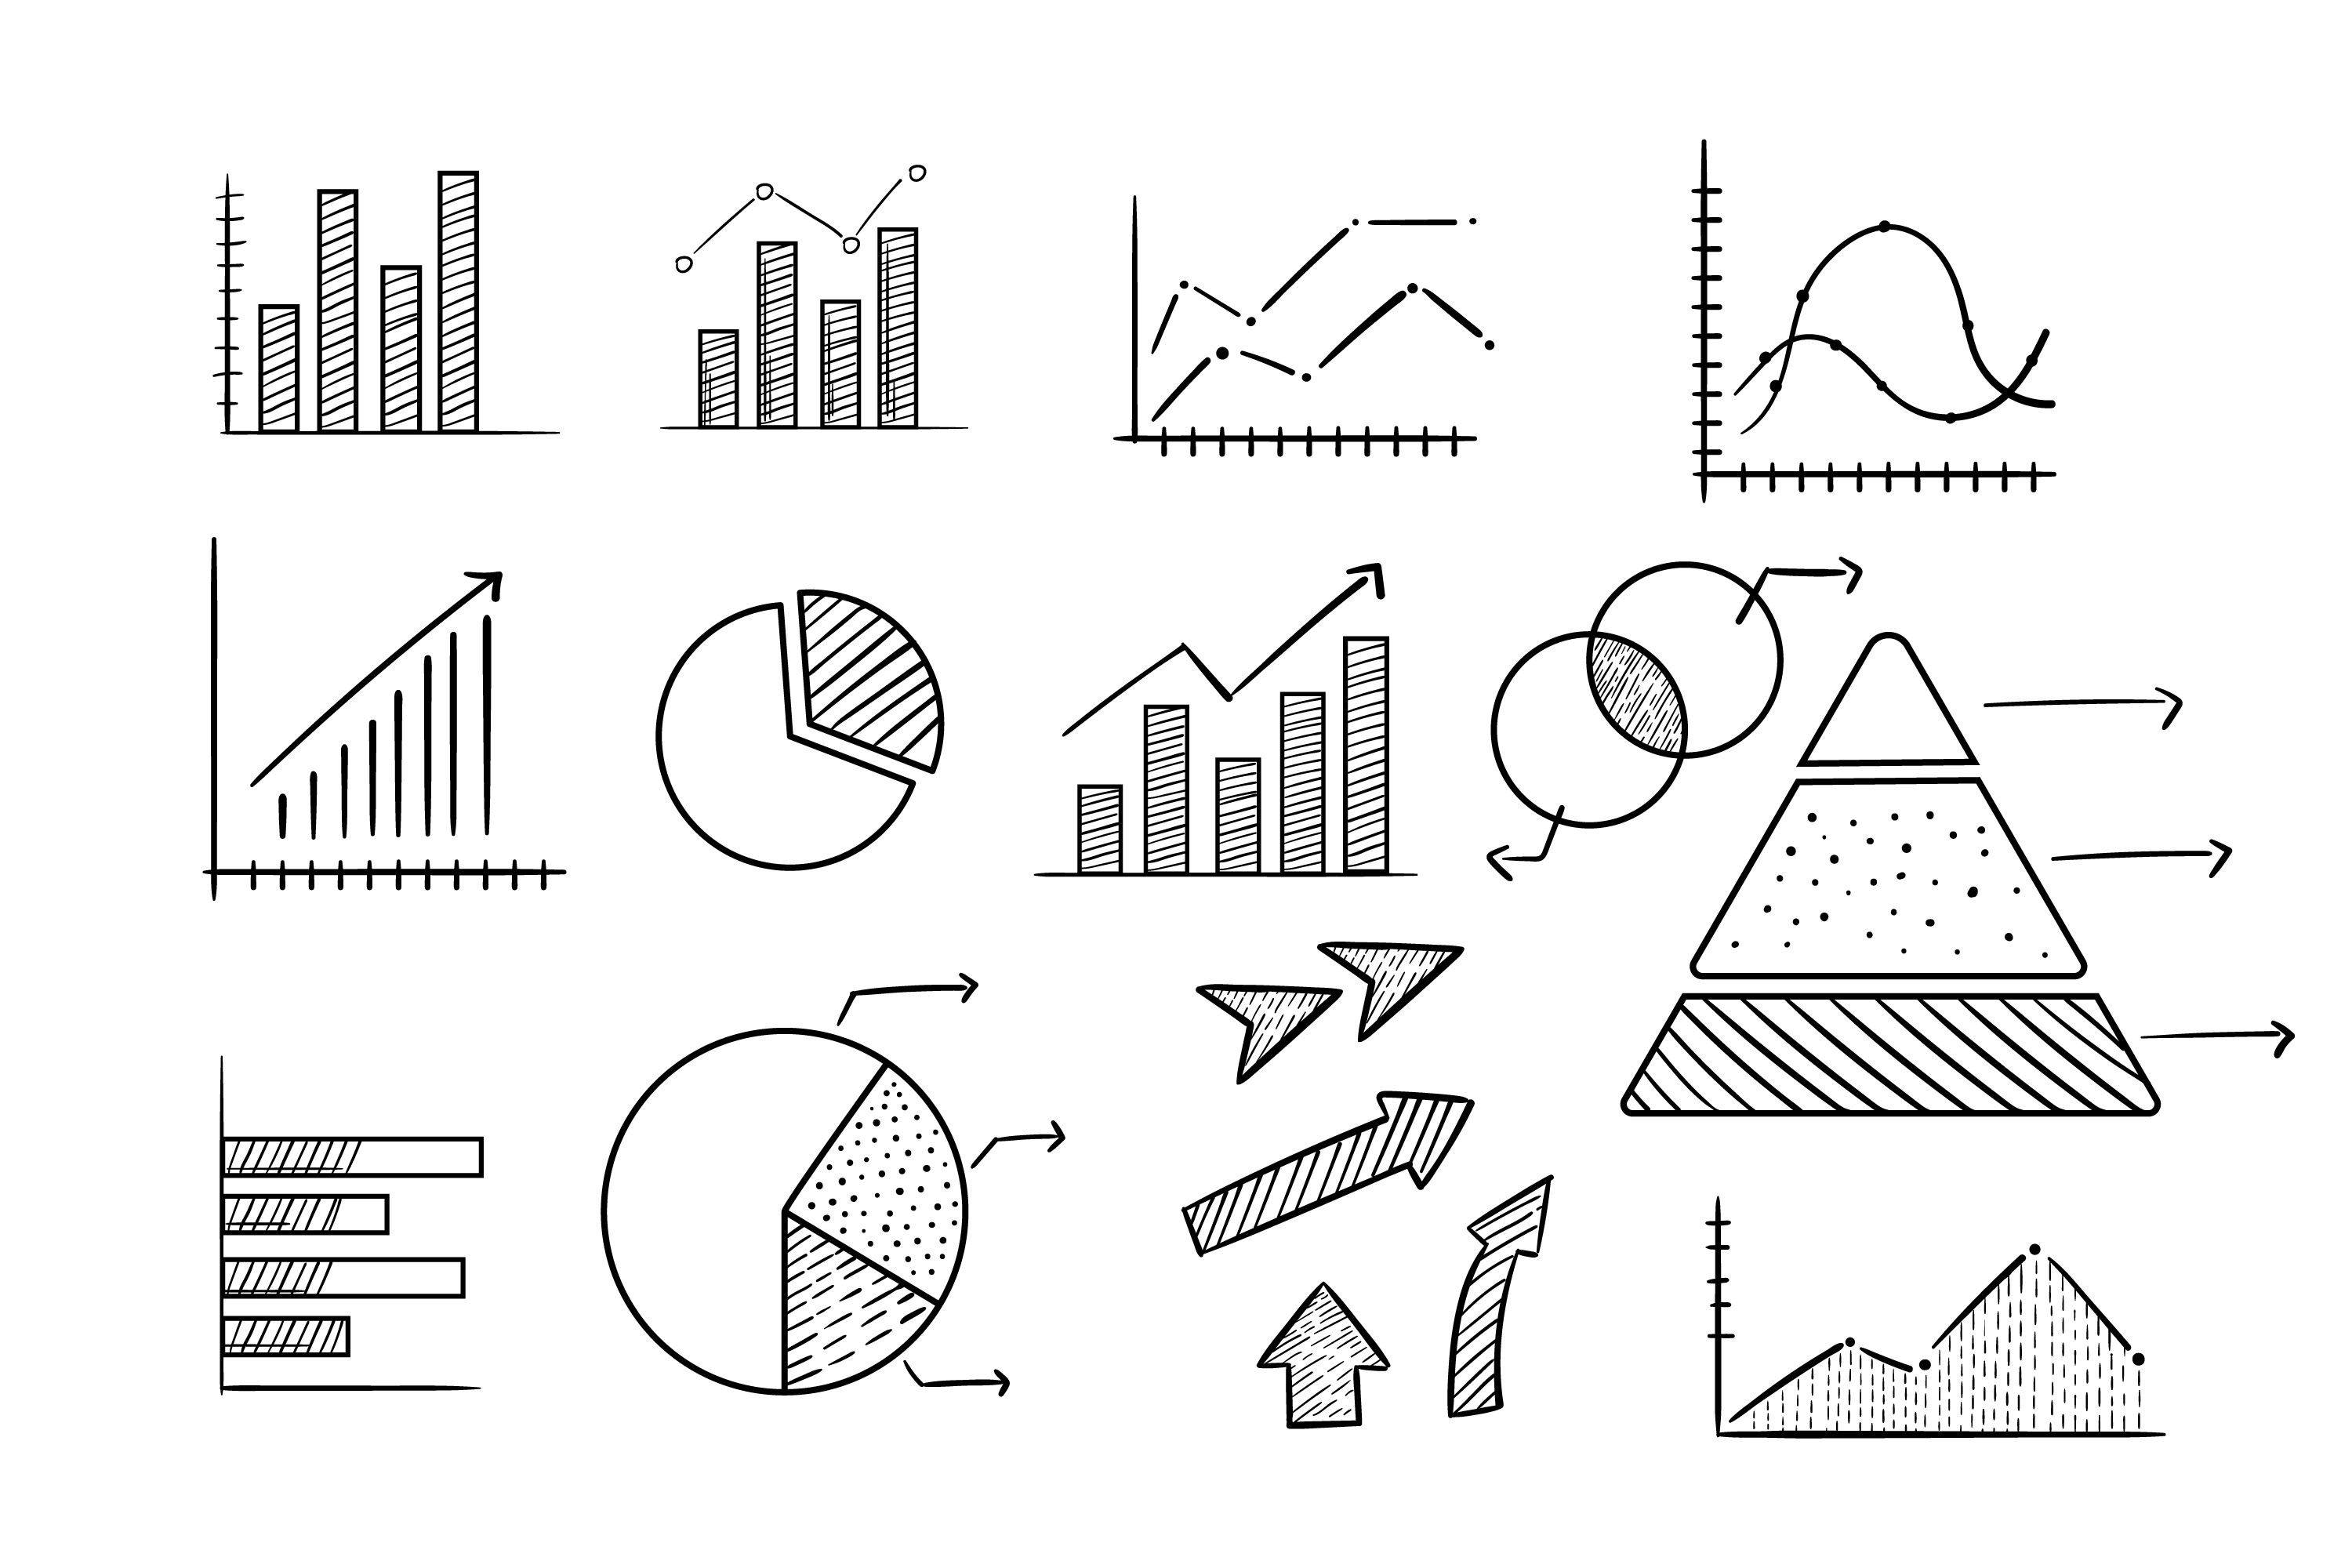
\includegraphics[width=3.92708in,height=0.8125in]{./imgSAEB_6_MAT/media/image135.png}
\end{figure}

Sabemos como representar dados, mas é hora de interpretar seu
significado. Por meio das medidas de tendência central, como a \textbf{média}, a \textbf{moda} e
a \textbf{mediana}, conseguimos entender as características centrais dos dados. Ao
calcular e compreender essas medidas, podemos extrair padrões valiosos e
inferir conclusões significativas.

Equipados com conhecimentos estatísticos, somos capazes de resolver problemas
complexos baseados em dados apresentados em tabelas ou gráficos. Além disso,
podemos desenvolver argumentos sólidos e analisar conclusões com base nessas
representações visuais dos dados, o que nos ajuda a tomar decisões informadas e
fundamentadas.

\begin{figure}[H]
\centering
\includegraphics[width=3.92708in,height=0.8125in]{./imgSAEB_6_MAT/media/image136.png}
\end{figure}

É preciso, ainda, explorar os passos necessários para realizar uma pesquisa
estatística ou um levantamento. Desde a formulação de perguntas até a
interpretação dos resultados, entenderemos o processo completo,
capacitando-nos a conduzir nossas próprias investigações no reino dos números.}

\section*{Atividades}

\num{1}  A tabela a seguir mostra o número de passageiros transportados por um
trem em determinada semana.

\begin{table}[H]\centering
\begin{tabular}[]{lr}
\toprule
Dia da semana & Número de passageiros\\
\midrule
Segunda-feira & $280$\\
Terça-feira & $187$\\
Quarta-feira & $211$\\
Quinta-feira & $198$\\
Sexta-feira & $291$\\
Sábado & $110$\\
Domingo & $87$\\
\bottomrule
\end{tabular}
\end{table}

Em que dia dessa semana o trem transportou mais passageiros?

\reduline{O trem transportou mais passagerios na sexta-feira.\hfill}

\num{2}  Em uma competição de natação, na prova dos $100$ m livres masculino, os
resultados estão descritos na tabela a seguir.

\begin{table}[H]\centering
\begin{tabular}{lllllllll}
Raia             & 1    & 2    & 3    & 4    & 5    & 6    & 7    & 8    \\
Tempo (segundos) & 46,6 & 47,8 & 45,5 & 45,1 & 46,5 & 47,4 & 48,2 & 50,1
\end{tabular}
\end{table}

Qual é a porcentagem de atletas que nadaram em um tempo superior a $46$
segundos?

\reduline{$75\%$ dos nadadores nadaram acima dos $46$ segundos.\hfill}

\num{3}  A imagem a seguir mostra um mapa de uma sala de aula representando a
cor favorita de cada aluno. Construa uma tabela indicando a frequência e
o percentual correspondente a cada cor.

\begin{figure}[h]
\centering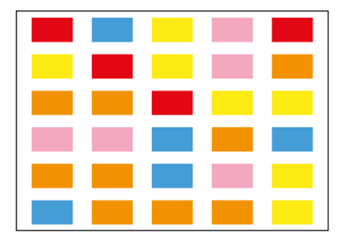
\includegraphics[width=3.52292in,height=2.45347in]{./imgSAEB_6_MAT/media/image82.png}
\end{figure}

%Paulo: criar tabela com as informações a seguir:

\begin{table}[H]\centering
\begin{tabular}{llr}
\toprule
Cores & Frequência & Porcentagem\\
\midrule
\Large{\rosa{Vermelho}} & \Large{\rosa{$4$}} & \Large{\rosa{$13,3$}}\\
\Large{\rosa{Azul}}     & \Large{\rosa{$5$}} & \Large{\rosa{$16,7$}}\\
\Large{\rosa{Amarelo}}  & \Large{\rosa{$7$}} & \Large{\rosa{$23,3$}}\\
\Large{\rosa{Rosa}}     & \Large{\rosa{$5$}} & \Large{\rosa{$16,7$}}\\
\Large{\rosa{Laranja}}  & \Large{\rosa{$9$}} & \Large{\rosa{$30,0$}}\\
\bottomrule
\end{tabular}
\end{table}

\num{4}  Um zoológico famoso contém em seu interior o total de $3.200$ animais
que estão separados por classes. Veja a tabela.

% Tabela
\begin{table}[h]\centering
\begin{tabular}[]{lr}
\toprule
Animais no zoológico &\\
\midrule
Classe & Quantidade de animais\\
Mamíferos & $479$\\
Aves & $1.620$\\
Répteis & $640$\\
Anfíbios & $340$\\
Invertebrados & $121$\\
\bottomrule
\end{tabular}
\end{table}

Observando os dados, calcule a porcentagem de

\begin{escolha}
\item mamíferos.

\reduline{$14,96875\%$.\hfill}
\item aves.

\reduline{$50,625\%$.\hfill}
\item répteis.

\reduline{$20\%$.\hfill}
\item anfíbios.

\reduline{$10,625\%$.\hfill}
\item invertebrados.

\reduline{$3,78125\%$.\hfill}
\end{escolha}

\num{5}  Leandro decidiu reorganizar suas atividades diárias semanais em uma
tabela, contendo a quantidade de horas de cada atividade.

\begin{table}[H]\centering
\begin{tabular}{lll}
Rotina                                  & Durante a semana & No fim de semana \\
Assistir à televisão                    & 3                & 3                \\
Fazer atividades domésticas             & 1                & 1                \\
Realizar atividades acadêmicas          & 5                & 1                \\
Ter tempo de lazer                      & 2                & 4                \\
Descansar, fazer higiene e alimentar-se & 10               & 12               \\
Fazer outras atividades                 & 3                & 3               
\end{tabular}
\end{table}

Após a reorganização, quantas horas por semana serão destinadas para
atividades acadêmicas?

\rosa{Deve-se usar a quantidade de horas e multiplicar pelos respectivos dias da semana:}

\rosa{Durante a semana:}

\rosa{$5 \text{horas} \cdot 5 \text{dias} = 25 \text{horas}$}

\rosa{No fim de semana:}

\rosa{$1 \text{horas} \cdot 2 \text{dias} = 2 \text{horas}$}

\rosa{Agora, somam-se os valores intermediários:}

\rosa{$25 + 2 = 27 \text{horas semanais}$}

\num{6}  O gráfico a seguir mostra a evolução mensal das vendas de certo
produto de julho a novembro de certo ano.

\begin{figure}[H]
\centering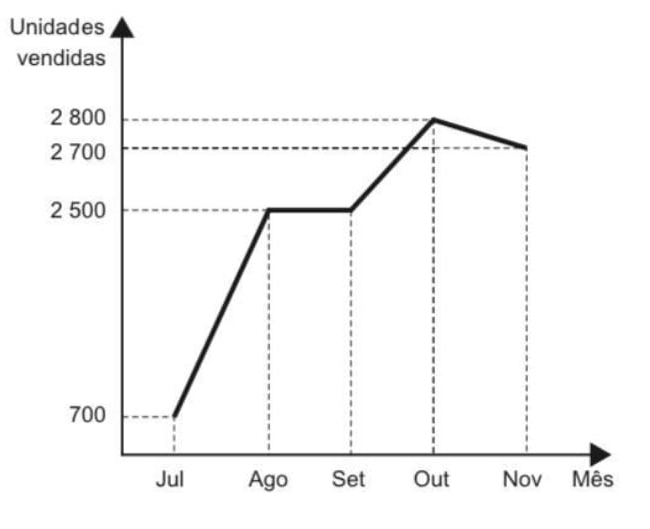
\includegraphics[width=3.36458in,height=2.73558in]{./imgSAEB_6_MAT/media/image84.png}
\end{figure}

Agora, responda ao que se pergunta a seguir.

\begin{escolha}
\item Em que mês mais unidades foram vendidas no período considerado?

\reduline{Outubro foi o mês de mais vendas no período.\hfill}

\item Em que mês menos unidades foram vendidas no período considerado?

\reduline{Julho foi o mês de menos vendas no período.\hfill}

\item Entre quais meses as vendas não se alteraram? Justifique.

\reduline{Entre agosto e setembro, as vendas não se alteraram, porque, nos dois meses
o número de unidades vendidas é o mesmo.\hfill}
\linhas{1}

\item Quantas unidades foram vendidas no total nesse período?

\reduline{$700 + 2.500 + 2.500 + 2.800 + 2.700 = 11.200 \text{unidades vendidas}$.\hfill}
\end{escolha}

\num{7} A seguir, aparece um gráfico de barras. Cada barra se refere a um mês. Os
meses estão marcados no eixo horizontal. O eixo vertical fornece o
número de bicicletas produzidas pela indústria em cada mês. Observe.

\begin{figure}[H]
\centering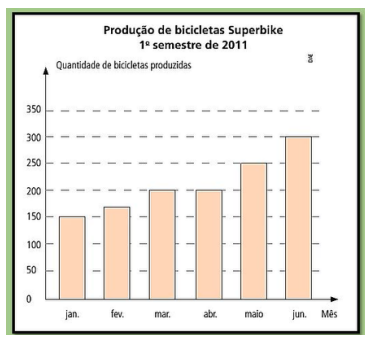
\includegraphics[width=3.875in,height=3.57292in]{./imgSAEB_6_MAT/media/image85.png}
\end{figure}

Agora, responda ao que se pergunta a seguir.

\begin{escolha}
\item Qual é o título do gráfico?

\reduline{Produção de bicicletas superbike 1° semestre de 2021\hfill}
\linhas{1}

\item Quantas bicicletas foram produzidas em janeiro?

\reduline{Foram produzidas $150$ unidades.\hfill}

\item Quantas bicicletas foram produzidas em maio?

\reduline{Foram produzidas $250$ unidades.\hfill}

\item Em que mês a produção de bicicletas foi maior?

\reduline{A produção foi maior em junho.\hfill}
\end{escolha}

\num{8} Cleuza é uma grande cozinheira. Ela sabe fazer vários tipos de
doce e salgado. Para organizar sua produção, ela fez uma tabela com as
encomendas da semana.

\begin{table}[H]\centering
\begin{tabular}{lll}
\textbf{Encomenda}     & \textbf{Doces} & \textbf{Salgados} \\
\textbf{Segunda-feira} & 123            & 111               \\
\textbf{Terça-feira}   & 755            & 242               \\
\textbf{Quarta-feira}  & 214            & 325               \\
\textbf{Quinta-feira}  & 320            & 147               \\
\textbf{Sexta-feira}   & 365            & 424               \\
\textbf{Sábado}        & 623            & 221               \\
\textbf{Domingo}       & 444            & 321              
\end{tabular}
\end{table}

Agora, responda ao que se pergunta a seguir.

\begin{escolha}
\item Em que dia da semana houve a maior encomenda?

\reduline{A maior encomenda ocorreu na terça-feira.\hfill}

\item Em que dia da semana houve a menor encomenda?

\reduline{A menor encomenda ocorreu na segunda-feira.\hfill}

\item Na quinta-feira, quantos salgados foram encomendados a mais que doces?

\reduline{$320 - 147 = 173 \text{salgados a mais}$.\hfill}

\item No domingo, a maior encomenda foi de doces ou de salgados? Quanto a mais

\reduline{$444 - 321 = 123 \text{salgados a mais}$.\hfill}
\end{escolha}

\num{9}  Observe no gráfico as vendas de uma sorveteria.

\begin{figure}[H]
\centering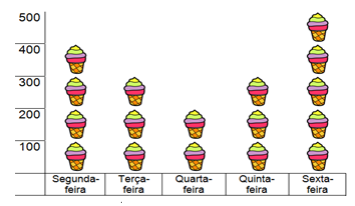
\includegraphics[width=3.7in,height=2.1in]{./imgSAEB_6_MAT/media/image87.png}
\end{figure}

Agora, responda ao que se pergunta a seguir.

\begin{escolha}
\item Quantos sorvetes foram vendidos no total?

\reduline{Segunda-feira: $400$; Terça-feira: $300$; Quarta-feira: $200$; Quinta-feira: $300$; Sexta-feira: $500$. Total: $1.700$.\hfill}

\item Quantos sorvetes foram vendidos na sexta-feira a mais que na quarta-feira?

\reduline{Foram vendidos $300$ sorvete a mais.\hfill}

\item Se na quarta-feira fosse vendido o dobro de sorvetes, esse valor seria
maior ou menor que o da sexta-feira?

\reduline{O valor seria menor.\hfill}
\end{escolha}

\num{10} Uma empresa de cosméticos lançou no mercado $5$ produtos diferentes:
A, B, C, D e E. O gráfico a seguir mostra o resultado de uma pesquisa feita para
verificar a preferência dos consumidores em relação a esses produtos.

\begin{figure}[H]
\centering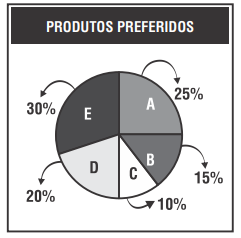
\includegraphics[width=2.51181in,height=2.47708in]{./imgSAEB_6_MAT/media/image88.png}
\end{figure}

Se foram entrevistados $2.400$ consumidores, quantos podemos afirmar que preferem o produto A?

\reduline{$600$ consumidores.\hfill}

\section*{Treino}

\num{1} Observe a figura.

\begin{figure}[H]
\centering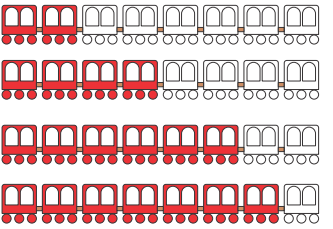
\includegraphics[width=3.46528in,height=2.38403in]{./imgSAEB_6_MAT/media/image89.png}
\end{figure}

O trenzinho em que $25\%$ dos vagões estão coloridos é o

\begin{escolha}
\item primeiro, de cima.
\item segundo, de cima para baixo.
\item terceiro, de cima para baixo.
\item quarto, de baixo.
\end{escolha}

%\subsection{BNCC: EF06MA31 }
% -- Identificar as variáveis e suas frequências e os
% elementos constitutivos (título, eixos, legendas, fontes e datas) em
% diferentes tipos de gráfico.
% SAEB: Representar ou associar os dados de uma pesquisa estatística ou de
% um levantamento em listas, tabelas (simples ou de dupla entrada) ou
% gráficos (barras simples ou agrupadas, colunas simples ou agrupadas,
% pictóricos, de linhas, de setores, ou em histograma).

% Gabarito
% Alternativa A: correta, pois $25\,\%$ de $8$ é igual a $2$.
% Alternativa B: incorreta, pois o aluno pode contar vagões a mais que não
% estão coloridos e chegar a essa conclusão.
% Alternativa C: incorreta, pois o aluno pode considerar realizar a conta
% sobre o represente de vagões que não estão coloridos.
% Alternativa D: incorreta, pois o aluno pode não compreender o conceito e
% frações e porcentagem e chegar a esse valor erroneamente.

\num{2}  Em um consultório médico, havia $4$ pessoas na sala de espera. O
atendimento da primeira pessoa durou $18$ minutos; o da segunda, $16$
minutos; o da terceira, $14$ minutos; o da quarta, $20$ minutos.
Qual foi o tempo médio de atendimento, por paciente, nesse consultório?

\begin{escolha}
\item $15$ minutos.
\item $16$ minutos.
\item $17$ minutos.
\item $68$ minutos.
\end{escolha}

%\subsection{BNCC: EF06MA32 }
% -- Interpretar e resolver situações que envolvam dados de
% pesquisas sobre contextos ambientais, sustentabilidade, trânsito,
% consumo responsável, entre outros, apresentadas pela mídia em tabelas e
% em diferentes tipos de gráficos e redigir textos escritos com o objetivo
% de sintetizar conclusões.
% SAEB: Interpretar o significado das medidas de tendência central (média
% aritmética simples, moda e mediana) ou da amplitude.

% Gabarito
% Alternativa A: incorreta, pois o aluno pode realizar o cálculo da
% mediana ao invés da media aritmética e chegar a essa conclusão.
% Alternativa b: incorreta, pois o aluno pode conspirar que o tempo esteja
% sendo modificado por uma P.A, de constante de mesmo valor subindo e
% descendo o tempo.
% Alternativa C: correta, pois utilizando a média aritmética $18 + 16 + 14$
% + $20 = 68$; 68/4 = $17$.
% Alternativa D: incorreta, pois o aluno pode somar todos os termos e
% esquecer de dividir chegando a esse valor.

\num{3}  Cada aluno de uma turma com $60$ alunos obteve nota $5$ ou nota $10$ em uma
lista de atividades. Se a média das notas foi $6$, quantos alunos
obtiveram nota $5$?

\begin{escolha}
\item $46$ alunos.
\item $48$ alunos.
\item $50$ alunos.
\item $52$ alunos.
\end{escolha}

%\subsection{BNCC: EF06MA32 }
% -- Interpretar e resolver situações que envolvam dados de
% pesquisas sobre contextos ambientais, sustentabilidade, trânsito,
% consumo responsável, entre outros, apresentadas pela mídia em tabelas e
% em diferentes tipos de gráficos e redigir textos escritos com o objetivo
% de sintetizar conclusões.
% SAEB: Interpretar o significado das medidas de tendência central (média
% aritmética simples, moda e mediana) ou da amplitude.

% Gabarito
% Alternativa A: incorreta, pois o aluno que não compreender corretamente
% o enunciado pode calcular $2$ notas a menos e chegar a esse resultado.
% Alternativa b: correta, pois o resultado final da média é $48$ alunos.
% Alternativa c: incorreta, pois o aluno que não compreender corretamente
% o enunciado pode calcular $2$ notas a mais e chegar a esse valor.
% Alternativa d: incorreta, pois o aluno que não compreender corretamente
% o enunciado pode calcular $4$ notas a mais e chegar a esse valor.
% erroneamente

\chapter{Grandezas e medidas}
\markboth{Módulo 11}{}

\section*{Habilidades do SAEB}

\begin{itemize}
\item
  Resolver problemas que envolvam medidas de grandezas (comprimento,
  massa, tempo, temperatura, capacidade ou volume) em que haja
  conversões entre unidades mais usuais.
\item
  Resolver problemas que envolvam perímetro de figuras planas.
\item
  Resolver problemas que envolvam área de figuras planas.
\item
  Resolver problemas que envolvam volume de prismas retos ou cilindros
  retos.
\end{itemize}

\subsection{Habilidade da BNCC} 

\begin{itemize}
\item EF06MA24.
\end{itemize}

\conteudo{As unidades de medida de comprimento surgem para padronizar as medidas
de distância. Existem várias unidades de medidas de comprimento. A
utilizada no sistema internacional de unidades é o metro, e seus
múltiplos (quilômetro, hectômetro e decâmetro) e submúltiplos
(decímetro, centímetro milímetro).

Além dessas unidades, existem outras, como as que utilizam o corpo como
parâmetro: o palmo, o pé, a polegada. Ainda, há aquelas que não são do
sistema internacional, mas são utilizadas a depender da região ou de
medidas astronômicas, como a légua, a jarda, a milha e o ano-luz.

\begin{figure}[H]
\centering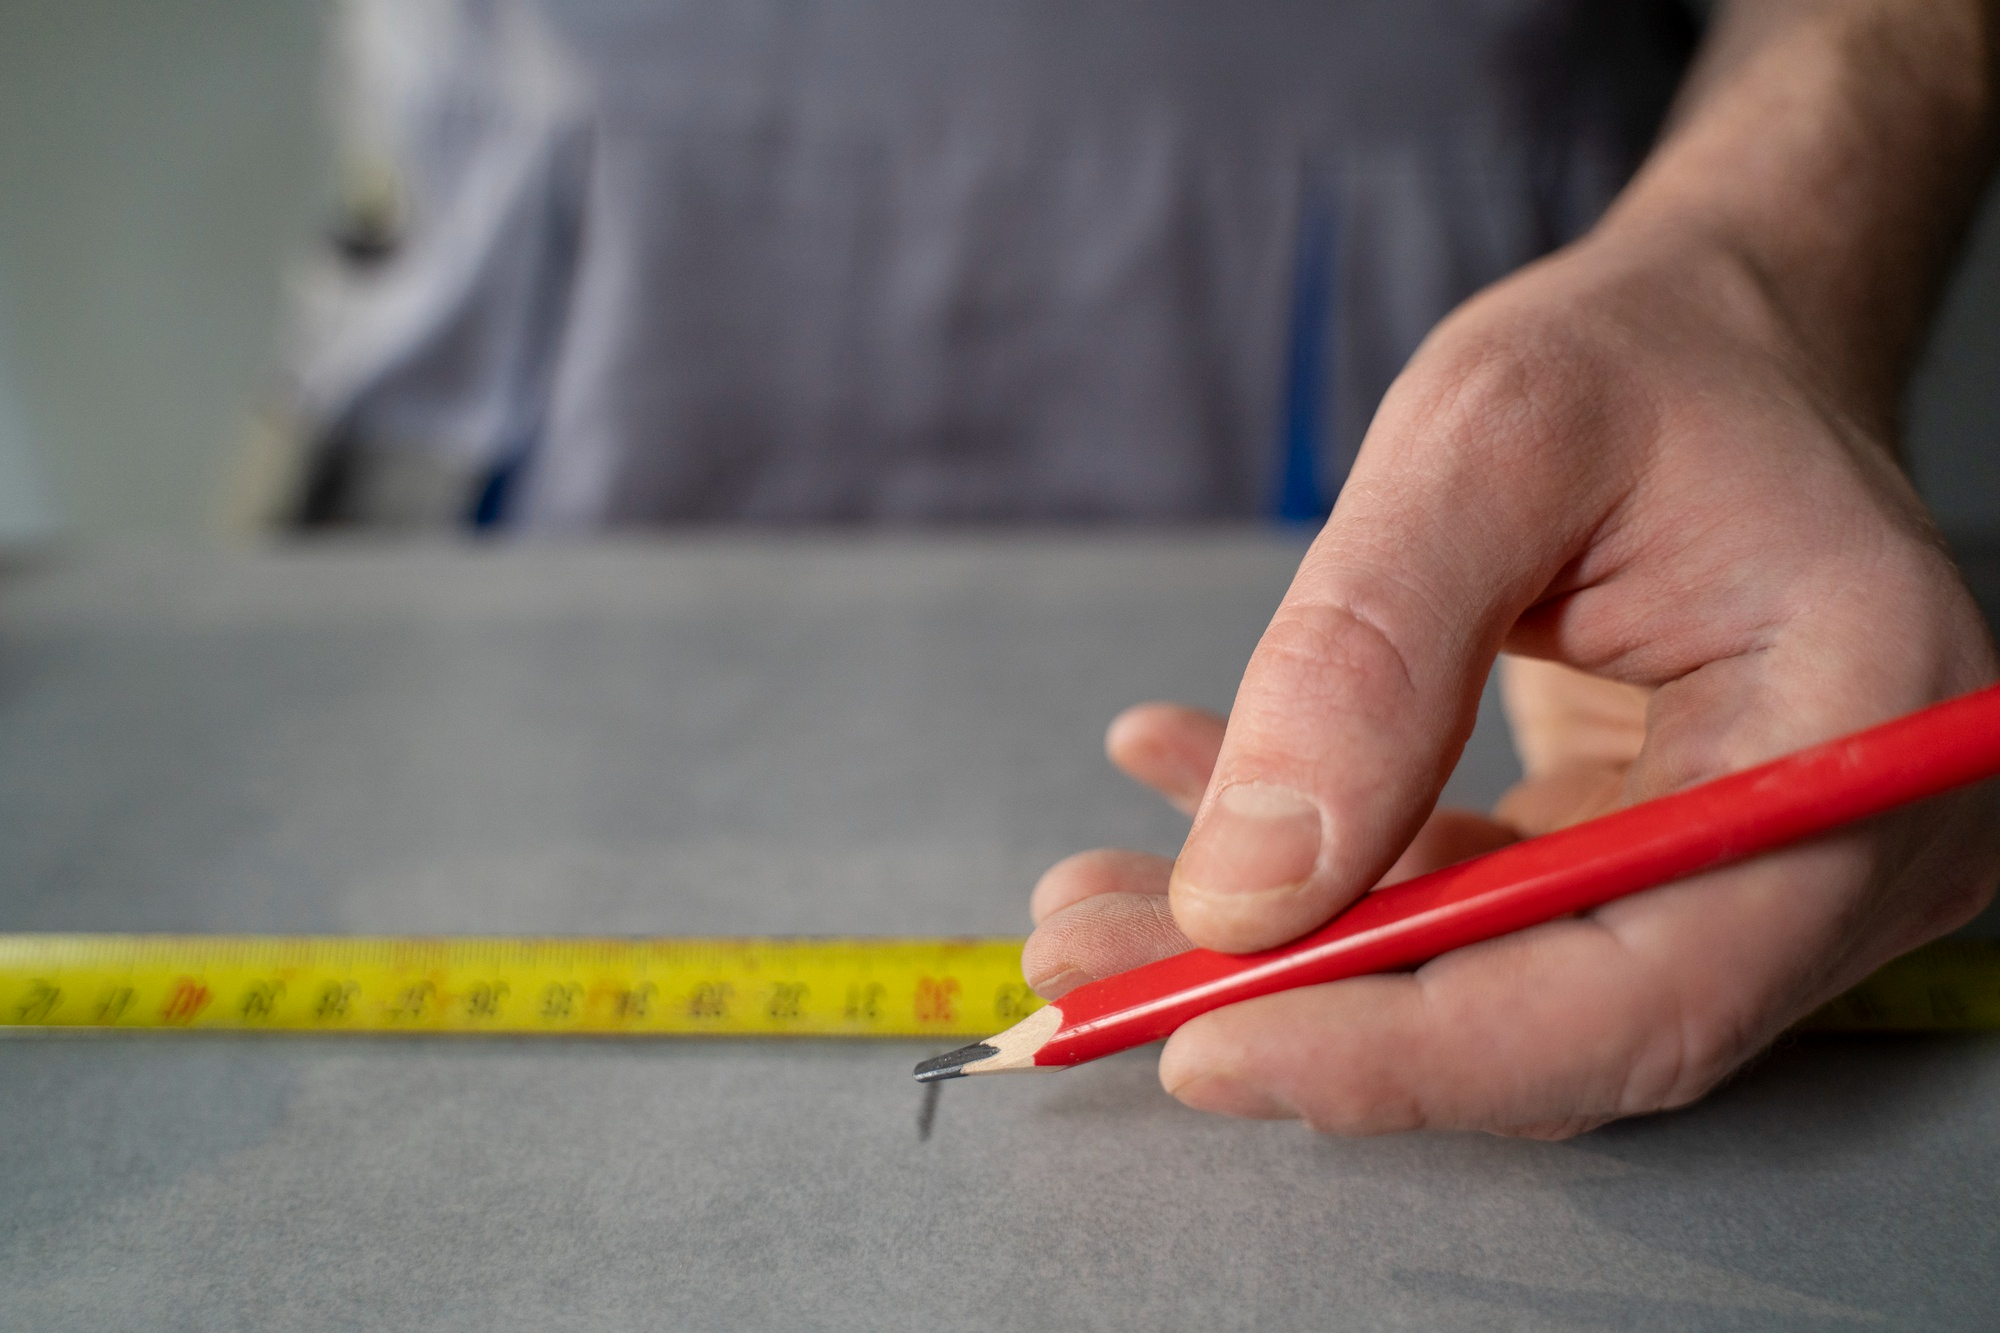
\includegraphics[width=3.92708in,height=0.8125in]{./imgSAEB_6_MAT/media/image137.png}
\end{figure}

Perímetro é uma medida que representa a soma das medidas de todos os
lados de uma figura plana. Em outras palavras, é a distância total ao
redor da figura.

O perímetro é uma medida importante para determinar a quantidade de
material necessário para cercar ou contornar uma figura, como no caso da
construção de cercas, muros, jardins, entre outros. Também é útil em
diversas áreas, como em geometria, construção civil, engenharia,
arquitetura, artes, entre outras.

O cálculo do perímetro varia de acordo com a figura geométrica. Para um
triângulo, basta somar as medidas dos três lados; para um quadrado,
basta multiplicar a medida de um dos lados por quatro; para um círculo, o
perímetro é chamado de circunferência e é calculado por meio da fórmula
$2 \cdot \pi \cdot \text{r}$, em que ``r'' representa o raio do círculo.

Já área é uma medida que quantifica o tamanho de uma superfície plana ou de
uma região delimitada por uma figura geométrica. A área é expressa em
unidades de medida quadradas, como metros quadrados (m²) ou centímetros
quadrados (cm²), por exemplo.

O cálculo da área varia de acordo com a figura geométrica em questão.
Por exemplo, para um retângulo, a área é calculada multiplicando a
medida da base pela medida da altura; para um círculo, a área é
calculada por meio da fórmula $\pi \cdot \text{r}^2$; para um
triângulo, a área é calculada pela metade do produto da base pela
altura; etc.

O volume de um prisma reto pode ser calculado multiplicando-se a área da
base do prisma pela sua altura. 
A área da base é a área da figura geométrica que forma a base do prisma.
A altura do prisma é a distância entre as bases paralelas do prisma.}

\section*{Atividades}

\num{1}  Uma lata de tinta, com a forma de um paralelepípedo retangular reto,
tem a base quadrada, com $24$ centímetros de lado, e altura de $40$ centímetros.
Calcule o volume máximo de tinta que a lata comporta.

\rosa{Para encontrar o volume máximo da lata de tinta, precisamos maximizar o volume}

\rosa{do paralelepípedo retangular reto. O volume de um paralelepípedo é dado pela}

\rosa{fórmula:}

\rosa{$V = A_{\text{base}} \times \text{altura}$}

\rosa{Neste caso, a base é quadrada, então a área da base ($A_{\text{base}}$) é}

\rosa{$24 \, \text{cm} \times 24 \, \text{cm} = 576 \, \text{cm}^2$, e a altura é}

\rosa{$40 \, \text{cm}$.}

\rosa{$V = 576 \, \text{cm}^2 \times 40 \, \text{cm} = 23040 \, \text{cm}^3$}

\rosa{Portanto, o volume máximo de tinta que a lata comporta é $23040 \, \text{cm}^3$}

\num{2}  Um condomínio contém uma cisterna de formato cilíndrico, com $3$ m de
altura e $2$ m de diâmetro. Qual é o volume máximo, em litros, de água que a cisterna
comporta? Utilize:$\pi = 3$.

\rosa{Para encontrar o volume máximo de água que a cisterna comporta, precisamos calcular o volume de um cilindro.}

\rosa{O volume ($V$) de um cilindro é dado pela fórmula:}

\rosa{$V = \pi \times \text{raio}^2 \times \text{altura}$}

\rosa{No caso da cisterna, o diâmetro é $2 \, \text{m}$, então o raio ($r$) é}

\rosa{$1 \, \text{m}$ ($2 \, \text{m} / 2 = 1 \, \text{m}$). A altura ($h$) é $3 \, \text{m}.}

\rosa{$V = 3 \times 1^2 \times 3 = 9 \, \text{m}^3$}

\rosa{Portanto, o volume máximo de água que a cisterna comporta é $9.000 \, \text{litros}$.}

\num{3} Em uma empresa, os setores alfa e beta fazem acordos diferentes
relativos à carga horária semanal de trabalho. O setor alfa trabalha $38$
horas por semana, enquanto o setor beta trabalha $44$ horas semanais.
Quantos minutos o setor beta trabalha a mais por semana do que o setor
alfa? 

\rosa{Para encontrar a diferença de tempo em minutos entre o setor beta e o setor alfa,}

\rosa{precisamos calcular a diferença nas horas de trabalho e, em seguida, converter essa diferença para minutos.}

\rosa{O setor alfa trabalha $38$ horas por semana, e o setor beta trabalha $44$ horas por semana.}

\rosa{A diferença em horas é: $44 \text{ horas} - 38 \text{ horas} = 6 \text{ horas}$}

\rosa{Para converter essas $6$ horas para minutos, multiplicamos por $60$ (porque há $60$ minutos em uma hora):}

\rosa{$6 \text{ horas} \times 60 \text{ minutos/hora} = 360 \text{ minutos}$}

\rosa{Portanto, o setor beta trabalha $360$ minutos a mais por semana do que o setor alfa.}

\num{4} Calcule o que se apresenta a seguir.

\begin{escolha}
\item A área de um quadrado de lado $13$ cm. \rosa{$169$ centímetros quadrados.}
\item O perímetro de um quadrado de lado $9$ cm. \rosa{$36$ centímetros.}
\item A área de um retângulo de lados $4$ cm e $5$ cm. \rosa{$20$ centímetros quadrados.}
\item O perímetro de um retângulo de lados $6$ cm e $4$ cm. \rosa{$20$ centímetros.}
\item A área de um círculo com diâmetro de $8$ cm ($\pi = 3$). \rosa{$48$ centímetros quadrados.}
\item O perímetro de um círculo com diâmetro de $20$ cm ($\pi = 3$). \rosa{$60$ centímetros.}
\end{escolha}

\begin{mdframed}[linewidth=2pt,linecolor=white,roundcorner=10pt]
\vspace{6cm}
\end{mdframed}

\num{5} Marina tem um terreno retangular de $3$ m por $6$ m e pretende cercá-lo
com $3$ voltas de arame farpado. Quantos metros de arame farpado ela precisa comprar
para fazer o que pretende?

\rosa{Para calcular a quantidade de arame farpado que Marina precisa comprar, primeiro, precisamos encontrar o perímetro do terreno. O perímetro de um retângulo é dado pela fórmula:}

\rosa{$\text{Perímetro} = 2 \times (\text{comprimento} + \text{largura})$}

\rosa{No caso de Marina, o terreno tem \(3\) metros de comprimento e \(6\) metros de largura. Portanto, o perímetro é:}

\rosa{$\text{Perímetro} = 2 \times (3 \, \text{m} + 6 \, \text{m}) = 2 \times 9 \, \text{m} = 18 \, \text{m}$}

\rosa{Marina pretende dar três voltas no terreno com o arame farpado. Então, a quantidade total de arame farpado que ela precisa comprar é:}

\rosa{$\text{Quantidade de arame farpado} = 3 \times \text{Perímetro} = 3 \times 18 \, \text{m} = 54 \, \text{m}$}

\rosa{Marina precisa comprar $54$ metros de arame farpado para cercar seu terreno com três voltas.}

\num{6}  Observe a temperatura registrada em um mesmo dia e horário em quatro
cidades do mundo.

\begin{table}[H]\centering
\begin{tabular}{llll}
\textbf{Paris (França)} & \textbf{Bangkok (Tailândia)} & \textbf{Barra Mansa (Brasil)} & \textbf{Oslo (Noruega)} \\
$-4\circ\text{C}$       & $33\circ\text{C}$            & $38\circ\text{C}$             & $-12\circ\text{C}$                  
\end{tabular}
\end{table}

Considerando apenas essas quatro cidades, a diferença entre a maior e a menor
temperatura, em $\circ\text{C}$, nesse dia, foi de quanto?

\rosa{Para encontrar a diferença entre a maior e a menor temperatura registrada nesse dia, você precisa encontrar a maior temperatura e a menor temperatura da tabela e então calcular a diferença entre elas.}

\rosa{A maior temperatura é $38^\circ\text{C}$ (em Barra Mansa, Brasil) e a menor temperatura é $-12^\circ\text{C}$ (em Oslo, Noruega).}

\rosa{A diferença entre a maior e a menor temperatura é:}

\rosa{$38^\circ\text{C} - (-12^\circ\text{C}) = 38^\circ\text{C} + 12^\circ\text{C} = 50^\circ\text{C}$}

\rosa{Portanto, a diferença entre a maior e a menor temperatura registrada nesse dia nessas quatro cidades foi de $50^\circ\text{C}$.}

\num{7} Em uma cidade, há uma praça retangular com $120$ metros de comprimento e
$80$ metros de largura. O prefeito da cidade decidiu construir uma fonte no centro
da praça em formato de cilindro reto. A base da fonte terá um diâmetro de $10$ metros
e a altura da fonte será de $6$ metros. Faça o que se pede a seguir.

\begin{escolha}
\item Calcule a área total da praça onde a fonte será construída.

    \rosa{A área total da praça é:}

    \rosa{$120 \, \text{m} \times 80 \, \text{m} = 9.600 \, \text{m}^2$}

    \rosa{A praça tem área de $9.600$ metros quadrados.}

\item Determine o perímetro da base da fonte e explique como chegou a esse valor.
Utilize $\pi = 3,14$.

    \rosa{O perímetro da base da fonte é a circunferência,}

    \rosa{que é $\pi \times \text{diâmetro} =$}

    \rosa{$= 3,14 \times 10 \, \text{m} =$}

    \rosa{$= 31,4 \, \text{m}$}

    \rosa{O perímetro da base da fonte é de $31,4$ metros.}

\item Determine o volume da fonte e explique como você chegou a essa resposta.

    \rosa{O volume da fonte é:}

    \rosa{$\pi \times \text{raio}^2 \times \text{altura}$}

    \rosa{$3,14 \times 5^2 \times 6 \, \text{m}$}

    \rosa{$471 \, \text{m}^3$}

\item Suponha que a fonte seja preenchida com água. Se cada metro cúbico de água
representa $1.000$ quilogramas, calcule a massa total da água na fonte, em toneladas.

    \rosa{O volume da água na fonte é:}

    \rosa{$471 \, \text{m}^3\)$}

    \rosa{Como $1 \, \text{m}^3$ de água representa $1.000 quilogramas,}

    \rosa{a massa total da água é $471 \times 1.000 = 471.000 \, \text{kg}$}

    \rosa{Para converter em toneladas, dividimos por $1.000$:

    \rosa{$471.000 \, \text{kg} ÷ 1.000 = 471 \, \text{toneladas}$}

\num{8} Uma placa avisa: é proibido som alto entre $22$ horas e $6$ horas.
Durante quantos minutos essa proibição deve ser respeitada?

\rosa{Para encontrar o número de minutos em que a proibição de som alto deve ser respeitada, primeiro, precisamos calcular o número de horas que a proibição está em vigor e, em seguida, converter essas horas em minutos.}

\rosa{A proibição está em vigor das $22$ horas até as $6$ horas do dia seguinte. Isso é um total de $8$ horas.}

\rosa{Para converter $8$ horas em minutos, multiplicamos por $60$, pois há $60$ minutos em $1$ hora:}

\rosa${8 \text{ horas} \times 60 \text{ minutos/hora} = 480 \text{ minutos}}$

\rosa{Portanto, a proibição de som alto deve ser respeitada durante $480$ minutos.}

\num{9} Pretende-se encher completamente um copo com um líquido, deixando-se
um espaço vazio de $0,5$ centímetro. O copo tem formato cilíndrico, e suas
medidas são: $10$ cm de altura e $4$ cm de diâmetro na base. Se $\pi = 3,14$,
qual é a quantidade aproximada (em mL) de líquido que cabe no copo?

\rosa{Para calcular o volume do líquido que cabe no copo, primeiro,}

\rosa{precisamos encontrar o volume total do copo e depois subtrair o espaço vazio.}

\rosa{O volume de um cilindro é dado pela fórmula $V = \pi r^2 h$, em que}

\rosa{$r$ é o raio da base e $h$ é a altura. Neste caso, $r = 2 \, \text{cm}$}

\rosa{(metade do diâmetro) e $h = 10 \, \text{cm}$. Substituindo esses valores na fórmula, temos:}

\rosa{$V_{\text{total}} = 3,14 \times 2^2 \times 10 = 3,14 \times 4 \times 10 = 125,6 \, \text{cm}^3$}

\rosa{Queremos deixar um espaço vazio de $0,5 \, \text{cm}$ no topo do copo.}

\rosa{Portanto, a altura efetiva do líquido no copo será $10 \, \text{cm} - 0,5 \, \text{cm} = 9,5 \, \text{cm}$.}

\rosa{O volume do líquido que cabe no copo é então:}

\rosa{$V_{\text{líquido}} = 3,14 \times 2^2 \times 9,5 = 3,14 \times 4 \times 9,5 = 119,2 \, \text{cm}^3$}

\rosa{Como $1 \, \text{cm}^3 = 1 \, \text{mL}$, a quantidade aproximada}

\rosa{de líquido que cabe no copo é $119,2 \, \text{mL}$.}

\num{10} A altura de uma vela mede $28 \text{cm}$ e, conforme ela é consumida, a
medida de sua altura diminui $1 \text{mm}$ a cada minuto.
Quanto tempo levará até a vela ser completamente consumida?

\rosa{Precisamos encontrar o tempo que levará para a vela ser completamente consumida,}

\rosa{dado que sua altura diminui $1 \, \text{mm}$ a cada minuto.}

\rosa{Inicialmente, a altura da vela é $28 \, \text{cm}$ ou $280 \, \text{mm}$.}

\rosa{A vela diminui $1 \, \text{mm}$ a cada minuto; então podemos usar a equação:}

\rosa{$\text{Altura restante} = 280 \, \text{mm} - 1 \, \text{mm} \times t \, \text{minutos}$}

\rosa{Queremos encontrar $t$ quando a altura restante é $0$;}

\rosa{portanto, podemos configurar a equação:}

\rosa{$280 \, \text{mm} - t \, \text{mm} = 0$}

\rosa{$t = 280 \, \text{minutos} = 4 \, \text{horas e } 40 \, \text{minutos}$}

\rosa{Levará $4 \, \text{horas e } 40 \, \text{minutos}$ para a vela ser completamente consumida.}

\num{11}  Observe as figuras apresentadas a seguir.

\begin{figure}[H]
\centering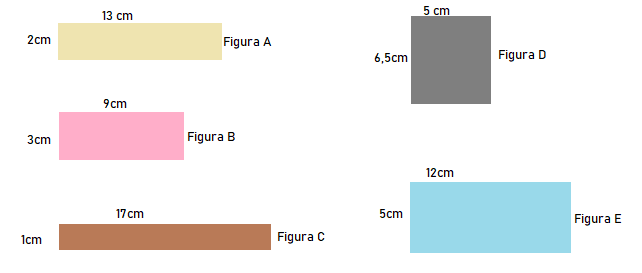
\includegraphics[width=5.90625in,height=2.51042in]{./imgSAEB_6_MAT/media/image98.png}
\end{figure}

Determine o perímetro e a área e cada figura.

\begin{escolha}
\item Figura A: \reduline{Perímetro: $30\,\text{cm}$. Área: $26\,\text{cm^2}$.\hfill}
\item Figura B: \reduline{Perímetro: $24\,\text{cm}$. Área: $27\,\text{cm^2}$.\hfill}
\item Figura C: \reduline{Perímetro: $36\,\text{cm}$. Área: $17\,\text{cm^2}$.\hfill}
\item Figura D: \reduline{Perímetro: $23\,\text{cm}$. Área: $32,5\,\text{cm^2}$.\hfill}
\item Figura E: \reduline{Perímetro: $34\,\text{cm}$. Área: $60\,\text{cm^2}$.\hfill}
\end{escolha}

\begin{mdframed}[linewidth=2pt,linecolor=white,roundcorner=10pt]
\vspace{6cm}
\end{mdframed}

\section*{Treino}

\num{1} Uma cooperativa agrícola produziu $36$ toneladas de feijão. Toda essa
produção será embalada em sacos de $120\,\text{kg}$ antes de ser transportada para
os distribuidores. Quantos sacos de feijão serão obtidos depois de
embalada toda a produção?

\begin{multicols}{2}
\begin{escolha}
\item $300$ sacos.
\item $30$ sacos.
\item $3$ sacos.
\item $3.000$ sacos.
\end{escolha}
\end{multicols}

%\subsection{BNCC: EF06MA24 }
% -- Resolver e elaborar problemas que envolvam as
% grandezas comprimento, massa, tempo, temperatura, área (triângulos e
% retângulos), capacidade e volume (sólidos formados por blocos
% retangulares), sem uso de fórmulas, inseridos, sempre que possível, em
% contextos oriundos de situações reais e/ou relacionadas às outras áreas
% do conhecimento.
% SAEB: Resolver problemas que envolvam medidas de grandezas (comprimento,
% massa, tempo, temperatura, capacidade ou volume) em que haja conversões
% entre unidades mais usuais.

% Gabarito
% Alternativa A: correta, pois realizamos o cálculo de $36.000$ : $120 = 300$
% Alternativa B: incorreta, pois o aluno pode converter erroneamente
% toneladas para\,kg e chegar a esse valor.
% Alternativa C: incorreta, pois o aluno pode converter erroneamente
% toneladas para\,kg e chegar a esse valor.
% Alternativa D: incorreta, pois o aluno pode converter erroneamente
% toneladas para\,kg e chegar a esse valor.

\num{2}  Observe a imagem.

\begin{figure}[H]
\centering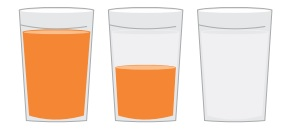
\includegraphics[width=2.98958in,height=1.38542in]{./imgSAEB_6_MAT/media/image100.png}
\end{figure}

Um copo cheio de água ``pesa'' $325\,\text{g}$. Se jogarmos metade da água fora, seu
``peso'' cai para $180\,\text{g}$. A massa do copo vazio é

\begin{escolha}
\item $145\,\text{g}$
\item $162,5\,\text{g}$
\item $35\,\text{g}$
\item $180\,\text{g}$
\end{escolha}

%\subsection{BNCC: EF06MA24 }
% -- Resolver e elaborar problemas que envolvam as
% grandezas comprimento, massa, tempo, temperatura, área (triângulos e
% retângulos), capacidade e volume (sólidos formados por blocos
% retangulares), sem uso de fórmulas, inseridos, sempre que possível, em
% contextos oriundos de situações reais e/ou relacionadas às outras áreas
% do conhecimento.
% SAEB: Resolver problemas que envolvam medidas de grandezas (comprimento, a)
% massa, tempo, temperatura, capacidade ou volume)
% entre unidades mais usuais.

% Gabarito
% Alternativa A: incorreta, pois o aluno pode realizar a subtração entre
% valores e chegar a esse valor.
% Alternativa B: incorreta, pois o aluno pode simplesmente dividir o valor
% 325 por $2$ e chegar a essa conclusão.
% Alternativa C: correta, pois a operação chega ao valor $35\,g$.
% Alternativa D: incorreta, pois o aluno pode simplesmente ler o enunciado
% e colocar esse valor como correto.

\num{3}  Oito quadrados iguais são colocados lado a lado, formando um
retângulo cujo perímetro é $72\,\text{cm}$. A área de cada quadrado que forma o
retângulo é

\begin{multicols}{2}
\begin{escolha}
\item $16\,\text{cm^2}$
\item $72\,\text{cm^2}$
\item $64\,\text{cm^2}$
\item $128\,\text{cm^2}$
\end{escolha}
\end{multicols}

%\subsection{BNCC: EF06MA24 }
% -- Resolver e elaborar problemas que envolvam as
% grandezas comprimento, massa, tempo, temperatura, área (triângulos e
% retângulos), capacidade e volume (sólidos formados por blocos
% retangulares), sem uso de fórmulas, inseridos, sempre que possível, em
% contextos oriundos de situações reais e/ou relacionadas às outras áreas
% do conhecimento.
% SAEB: Resolver problemas que envolvam medidas de grandezas (comprimento,
% massa, tempo, temperatura, capacidade ou volume) em que haja conversões
% entre unidades mais usuais.

% Gabarito
% Alternativa A: correta, pois a operação matemática a partir da fórmula
% da área chega ao valor $16cm^2$.
% Alternativa B: incorreta, pois o aluno pode considerar que o perímetro e
% a área sejam iguais e chegar a essa conclusão.
% Alternativa C: incorreta, pois o aluno pode erroneamente dividir o
% retângulo em $2$, descobrindo essa área incorretamente.
% Alternativa D: incorreta, pois o aluno pode considerar a área final do
% retângulo ao invés da área de cada quadrado.

\chapter{Probabilidade}
\markboth{Módulo 12}{}

\section*{Habilidade do SAEB}
\begin{itemize}
\item Resolver problemas que envolvam a probabilidade de
ocorrência de um resultado em eventos aleatórios equiprováveis
independentes ou dependentes.
\end{itemize}

\subsection{Habilidade da BNCC} 
\begin{itemize}
\item EF06MA30.
\end{itemize}

\conteudo{A probabilidade é uma medida numérica que expressa a chance de um evento
ocorrer. É uma forma de quantificar a incerteza em uma situação. A
probabilidade é expressa como um número entre $0$ e $1$, sendo $0$ a
probabilidade de um evento impossível e $1$ a probabilidade de um evento
certo.

Por exemplo, se lançarmos uma moeda, a probabilidade de que ela caia com
a face ``cara'' para cima é de $0,5$ (ou $50\%$). Isso significa que, em uma
série de lançamentos de moedas, espera-se que a face ``cara'' apareça em
cerca de metade das vezes.

\begin{figure}[H]
\centering
\includegraphics[width=3.92708in,height=0.8125in]{./imgSAEB_6_MAT/media/image138.png}
\end{figure}

A probabilidade pode ser calculada por meio da razão entre o número de
eventos favoráveis e o número total de eventos possíveis. Por exemplo,
se lançarmos um dado de seis faces, a probabilidade de que ele caia com
a face $3$ para cima é de $\frac{1}{6}$, pois há apenas uma face com o número $3$ e
seis faces no total.

A probabilidade também pode ser calculada a partir da frequência com que
um evento ocorre em uma série de experimentos. Por exemplo, se jogarmos
um dado várias vezes e o número $3$ aparecer em $20\%$ dos lançamentos,
podemos estimar que a probabilidade de obter o número $3$ em um lançamento
único é de, aproximadamente, $0,2$.}

\section*{Atividades}

\num{1}  Uma moeda é lançada três vezes. Qual é a probabilidade de

\begin{escolha}
\item sair \textbf{exatamente} uma cara?

\reduline{$\frac{3}{8}$.\hfill}

\item sair \textbf{pelo menos} uma cara?

\reduline{$\frac{7}{8}$.\hfill}
\end{escolha}

\num{2}  Dois dados foram lançados. Qual é a probabilidade de a soma dos
pontos obtidos ser

\begin{escolha}
\item igual a 8?

\reduline{$\frac{5}{36}$.\hfill}

\item maior que 8?

\reduline{$\frac{5}{18}$.\hfill}
\end{escolha}

\num{3} Imagine que você está participando de um jogo de tabuleiro chamado
´´Lançamento de dados mágicos''. Nesse jogo, você tem dois dados mágicos,
cada um com faces numeradas de $1$ a $6$. O objetivo é somar os números
obtidos nos dois dados e alcançar uma pontuação específica. As regras são
as seguintes.

\begin{itemize}
   \item Você ganha automaticamente se a soma dos números nos dois dados for $12$.
   \item Se a soma for $7$ ou $11$, você ganha com uma probabilidade de $\frac{1}{6}$.
   \item Se a soma for $2$, $3$ ou $4$, você ganha com uma probabilidade de $\frac{1}{12}$.
   \item Para todas as outras somas, você perde.
\end{itemize}

Agora, faça o que se pede a seguir.

\begin{escolha}
\item Calcule a probabilidade de ganhar o jogo.

\rosa{Para ganhar o jogo, existem três cenários favoráveis:}

\rosa{Soma 12: há apenas uma combinação possível: (6, 6).}

\rosa{Soma 7: há seis combinações possíveis: (1, 6), (2, 5), (3, 4), (4, 3), (5, 2) e (6, 1).}

\rosa{Soma 11: há duas combinações possíveis: (5, 6) e (6, 5).}

\rosa{Soma 2: há uma combinação possível: (1, 1).}

\rosa{Soma 3: há duas combinações possíveis: (1, 2) e (2, 1).}

\rosa{Soma 4: há três combinações possíveis: (1, 3), (2, 2) e (3, 1).}

\rosa{A probabilidade total de ganhar é a soma das probabilidades de cada cenário:}

\rosa{$P(\text{Ganhar}) = \frac{1}{36} + \frac{8}{36} + \frac{6}{36} = \frac{15}{36} = \frac{5}{12}$}

\item Calcule a probabilidade de perder o jogo.

\rosa{Para perder o jogo, a soma deve ser qualquer número que não esteja nos cenários de vitória.}

\rosa{Existem $6 \times 6 = 36$ resultados possíveis ao lançar dois dados.}

\rosa{$P(\text{Perder}) = 1 - P(\text{Ganhar}) = 1 - \frac{5}{12} = \frac{7}{12}$}

\item Se você já sabe que não perdeu o jogo, qual é a probabilidade de ter ganhado?

\rosa{Se você não perdeu o jogo, então a soma deve ser 2, 3, 4, 7, 11 ou 12.}

\rosa{Entre essas, há 15 combinações que levam à vitória.}

\rosa{$P(\text{Ganhar} \,|\, \text{Não perder}) = \frac{15}{15 + 5} = \frac{15}{20} = \frac{3}{4}$}

\item Suponha que você possa apostar dinheiro nesse jogo. Você deve apostar?
Explique sua resposta considerando as probabilidades de ganhar e perder.

\reduline{Considerando as probabilidades, apostar dinheiro nesse jogo não é uma decisão sábia. A probabilidade de perder ($\frac{7}{12}$) é maior do que a probabilidade de ganhar ($\frac{5}{12}$). Portanto, a longo prazo, você tende a perder mais do que ganhar se continuar apostando.}
\linhas{3}
\end{escolha}

\num{4}  Uma urna contém cem bolinhas numeradas de $1$ a $100$. Uma bolinha é
escolhida, e é observado seu número. Admitindo probabilidades iguais a
$\frac{1}{100}$ para todos os eventos elementares, qual é a probabilidade de
observarmos um

\begin{escolha}
\item múltiplo de $6$ e de $8$ simultaneamente?

\reduline{$\frac{1}{25}$.\hfill}

\item múltiplo de $6$ ou de $8$?

\reduline{$\frac{6}{25}$.\hfill}

\item número não múltiplo de $5$?

\reduline{$\frac{4}{5}$.\hfill}
\end{escolha}

\num{5}  Uma urna contém seis bolas pretas, duas brancas e dez amarelas.
Uma bola é escolhida ao acaso na urna. Qual é a probabilidade de a bola

\begin{escolha}
\item não ser amarela?

\reduline{$\frac{4}{9}$.\hfill}

\item ser branca ou preta?

\reduline{$\frac{4}{9}$.\hfill}

\item não ser branca nem amarela?

\reduline{$\frac{1}{3}$.\hfill}
\end{escolha}

\num{6} Num grupo de $500$ estudantes, $80$ estudam Engenharia, $150$ estudam
Economia e $10$ estudam Engenharia e Economia. Se um aluno é escolhido ao
acaso, qual é a probabilidade de que ele

\begin{escolha}
\item estude somente Engenharia?

\reduline{$\frac{7}{50}$.\hfill}
\item estude somente Economia?

\reduline{$\frac{7}{25}$.\hfill}
\item não estude Engenharia nem Economia?

\reduline{$\frac{14}{25}$.\hfill}
\item estude Engenharia ou Economia?

\reduline{$\frac{11}{25}$.\hfill}
\end{escolha}

\num{7}  De um grupo de $200$ pessoas, $160$ têm fator Rh positivo, $100$ têm sangue
tipo O e $80$ têm fator Rh positivo e sangue tipo O. Se uma dessas pessoas
for selecionada ao acaso, qual a probabilidade de:

\begin{escolha}
\item Seu sangue ter fator Rh positivo? \reduline{$4/5$.\hfill}
\item Seu sangue não ser tipo O? \reduline{$1/2$.\hfill}
\item Seu sangue ter fator Rh positivo ou ser tipo O? \reduline{$9/10$.\hfill}
\end{escolha}

\num{8}  Na loteria são sorteadas $5$ dezenas distintas dentre as dezenas $00$,
01, $02$, $03$, ..., $99$. Um apostador escolhe $10$ dezenas. Determine a
probabilidade dele fazer:

\begin{escolha}
\item Um terno. \reduline{$0,638353\%$.\hfill}
\item Uma quadra. \reduline{$0,025104\%$.\hfill}
\item A quina. \reduline{$0,000335\%$.\hfill}
\end{escolha}

\num{9}  Com os dígitos $1$, $2$, $3$, $4$, $5$ são formados números de $4$ algarismos
distintos. Um deles é escolhido ao acaso. Qual é a probabilidade de ele
ser:

\begin{escolha}
\item Par. \reduline{$2/5$.\hfill}
\item Ímpar. \reduline{$3/5$.\hfill}
\end{escolha}

\num{10} Oito pessoas (entre elas Pedro e Silvia) são dispostas ao acaso numa
fila. Qual a probabilidade de:

\begin{escolha}
\item Pedro e Silvia ficarem juntos? \reduline{$1/4$.\hfill}
\item Pedro e Silvia ficarem separados? \reduline{$3/4$.\hfill}
\end{escolha}

\num{11} Uma urna contém $5$ bolas vermelhas e $3$ brancas. Duas bolas são
extraídas ao acaso, com reposição. Qual é a probabilidade de:

\begin{escolha}
\item Ambas serem vermelhas? \reduline{$25/64$.\hfill}
\item Ambas serem brancas? \reduline{$9/64$.\hfill}
\end{escolha}

\section*{Treino}

\num{1}  Na lanchonete, você pode escolher entre $4$ tipos de pães para seu
sanduíche: pão de forma, pão francês, pão sírio e pão preto. Você pode
escolher também $5$ tipos de recheios: mortadela, queijo, presunto, peito
de peru ou peito de frango. De quantas maneiras diferentes você pode
pedir seu sanduíche com apenas um recheio?

\begin{escolha}
\item $20$ maneiras.
\item $9$ maneiras.
\item $1.024$ maneiras.
\item $1$ maneira.
\end{escolha}

%\subsection{BNCC: EF06MA30 }
% -- Calcular a probabilidade de um evento aleatório,
% expressando-a por número racional (forma fracionária, decimal e
% percentual) e comparar esse número com a probabilidade obtida por meio
% de experimentos sucessivos.
% SAEB: Resolver problemas que envolvam a probabilidade de ocorrência de
% um resultado em eventos aleatórios equiprováveis independentes ou
% dependentes.

% Gabarito
% Alternativa A: correta, pois $4 x 5 = 20$ maneiras.
% Alternativa B: incorreta pois, o aluno pode realizar a soma ao invés da
% multiplicação.
% Alternativa C: incorreta, pois o aluno pode realizar a potenciação ao
% invés da multiplicação.
% Alternativa D: incorreta, pois o aluno pode realizar a subtração ao
% invés da multiplicação.

\num{2}  Dona Josefa vende bolas de sorvete em sua casa. Ela oferece $6$ sabores
aos seus clientes: chocolate, uva, morango, creme, limão e flocos.
Geralmente, seus clientes pedem duas bolas. Quantas combinações de duas
bolas são possíveis com esses sabores de sorvete?

\begin{escolha}
\item $1$ combinação
\item $46.656$ combinações
\item $36$ combinações
\item $12$ combinações
\end{escolha}

%\subsection{BNCC: EF06MA30 }
% -- Calcular a probabilidade de um evento aleatório,
% expressando-a por número racional (forma fracionária, decimal e
% percentual) e comparar esse número com a probabilidade obtida por meio
% de experimentos sucessivos.
% SAEB: Resolver problemas que envolvam a probabilidade de ocorrência de
% um resultado em eventos aleatórios equiprováveis independentes ou
% dependentes.

% Gabarito
% Alternativa A: incorreta, pois o aluno pode realizar a soma ao invés da
% multiplicação e chegar a esse resultado.
% Alternativa b: incorreta, pois o aluno pode realizar uma potenciação ao
% invés da multiplicação. 
% Alternativa C: correta, pois são possíveis $36$ combinações.
% Alternativa D: incorreta, pois o aluno pode realizar uma soma ao invés
% da multiplicação.

\num{3}  Suponha que em uma urna haja $10$ bolas numeradas de $1$ a $10$. Qual é a
probabilidade de se retirar uma bola com número par?

\begin{escolha}
\item $0,2$
\item $0,5$
\item $0,6$
\item $0,8$
\end{escolha}

%\subsection{BNCC: EF06MA30 }
% -- Calcular a probabilidade de um evento aleatório,
% expressando-a por número racional (forma fracionária, decimal e
% percentual) e comparar esse número com a probabilidade obtida por meio
% de experimentos sucessivos.
% SAEB: Resolver problemas que envolvam a probabilidade de ocorrência de
% um resultado em eventos aleatórios equiprováveis independentes ou
% dependentes.

% Gabarito
% Alternativa A: incorreta, pois o aluno pode ter considerado apenas dois
% números.
% Alternativa B: correta, pois há cinco números pares entre um total de
% 10.
% Alternativa C: incorreta, incorreta, pois o aluno pode ter considerado
% seis números.
% alternativa D: incorreta, pois incorreta, pois o aluno pode ter
% considerado oito números.


